\documentclass[openany,twoside, notitlepage,letterpaper,11pt]{book}

%%% These are the packages that are used
%used for custom page headers and page numbering
\usepackage{fancyhdr}

%adds TeX fonts from the American Mathematical Society.
\usepackage{amsfonts}

%Sets the bounds of the page margins
\usepackage[top=1in, bottom=1in, left=0.7in, right=.7in]{geometry}

%Various useful packages
\usepackage{amsmath,amssymb, amscd,amsbsy, amsthm, enumerate}
\usepackage{mdframed, titlesec, setspace,verbatim, multicol, caption}
\usepackage[unicode]{hyperref}
\usepackage{wasysym}
\usepackage{tikz, polynom}
\usepackage{xcolor}
\usepackage{etoolbox}

%enables the ability of including pages from a pdf.
\usepackage{pdfpages}

%enables drawings of circuit diagrams
\usepackage{circuitikz}

%enables indexing
\usepackage{makeidx} 

%enables changing the bibliography name
\usepackage[nottoc,notlof,notlot]{tocbibind}

%makes the index size footnote
\usepackage[font=footnotesize, columns=3]{idxlayout}

%Adds extra symbols
\usepackage{mathrsfs, upgreek}

%Allows for tables with cells that span multiple rows and columns
\usepackage{multirow}



%This is where settings for the latex file are stored.
%%Version Number
\newcommand{\Version}{0.001}
%%Version

%%% Page formatting
%\setlength{\headsep}{30pt}
\setlength{\parindent}{25pt}
\setlength{\textheight}{9in}

%Rename the bibliography to References.
\renewcommand\bibname{References}


%%% Header and Footer Info
\pagestyle{fancy}
\fancyhead[LO]{\small {\textbf{Antonius' Compendium -- Volume I. Version \Version}}}
\fancyhead[RE]{\small {\textbf{Antonius' Compendium -- Volume I. Version \Version}}}
\fancyhead[C]{}
\fancyhead[RO]{\small \thepage}
\fancyhead[LE]{\small \thepage}
\fancyfoot[L]{}
\fancyfoot[C]{}
\fancyfoot[R]{}


\patchcmd{\chapter}{plain}{empty}{}{}
\titleformat{\chapter}[display]
{\normalfont\huge\bfseries}{}{0pt}{\Huge}
\titlespacing*{\chapter} {0pt}{-50pt}{10pt}

%re-defines the plain page style
\fancypagestyle{plain}{%
	\fancyhf{}
	\rhead{\thepage}
	\renewcommand{\headrulewidth}{0pt}}

%This is where custom definitions and variables are defined and stored.
\newcommand{\andspace}[1]{\hspace{#1}\textrm{and}\hspace{#1}}

\numberwithin{equation}{section}
\setlength{\columnsep}{.5cm}
\setlength{\columnseprule}{1pt}
\def\columnseprulecolor{\color{black}}

\newcommand{\abs}[1]{\left| #1 \right|}
\newcommand{\inner}[1]{\langle #1 \rangle}
\newcommand{\norm}[1]{\left\lVert#1\right\rVert}
\newcommand{\spanvect}{\textnormal{span}}
\newcommand{\union}{\cup}
\newcommand{\Union}{\bigcup}

% Defines a keyword which will bold and add a word to the index.
\newcommand{\keyword}[1]{\textbf{#1}\index{#1}}

% Create a section without making the section title.
\newcommand\invisiblesection[1]{%
	\refstepcounter{section}%
	\addcontentsline{toc}{section}{\protect\numberline{\thesection}#1}%
	\sectionmark{#1}}

% Makes a chapter with no title
\makeatletter
\newcommand{\unchapter}[1]{%
	\begingroup
	\let\@makechapterhead\@gobble % make \@makechapterhead do nothing
	\chapter{#1}
	\endgroup
}
\makeatother

%%% These are some shortcuts that are handy
\def\real{{\mathbb R}}
\def\Natural{\mathbb{N}}
\def\dx{\textnormal{dx}}
\def\dy{\textnormal{dy}}
\def\dz{\textnormal{dz}}
\def\dt{\textnormal{dt}}
\def\ds{\textnormal{ds}}
\def\dw{\textnormal{dw}}
\def\Re{\textnormal{Re}}
\def\Im{\textnormal{Im}}
\def\exp{\textnormal{exp}}
\def\interior{\textnormal{interior}}
\def\al{\alpha}
\def\del{\delta}
\def\Del{\Delta}
\def\gam{\gamma}
\def\Gam{\Gamma}
\def\Om{\Omega}
\def\ep{\varepsilon}
\def\lam{\lambda}
\def\rational{{\mathbb Q}}
\def\integer{{\mathbb Z}}
\def\Q{{\mathbb Q}}
\def\Z{{\mathbb Z}}
\def\N{{\mathbb N}}
\def\R{{\mathbb R}}
\def\grad{\nabla}
\def\C{\mathcal C}
\def\P{\mathcal P}
\def\T{\mathcal T}
\def\I{\mathcal I}
\def\intersect{\cap}
\def\Intersect{\bigcap}


%%% This defines the solution environment for you to write your solutions
\newenvironment{soln}
{\let\oldqedsymbol=\qedsymbol
	\renewcommand{\qedsymbol}{$ $}
	\begin{proof}[\bfseries\upshape \color{blue}Derivation]\color{blue}}
	{\end{proof}
	\renewcommand{\qedsymbol}{\oldqedsymbol}}

\newenvironment{note}
{\let\oldqedsymbol=\qedsymbol
	\renewcommand{\qedsymbol}{$ $}
	\begin{proof}[\bfseries\upshape \color{red}Note]\color{red}}
	{\end{proof}
	\renewcommand{\qedsymbol}{\oldqedsymbol}}
	

\newenvironment{Deletion}
{\let\oldqedsymbol=\qedsymbol
	\renewcommand{\qedsymbol}{$ $}
	\begin{proof}[\bfseries\upshape \color{red}Deletion]\color{red}}
	{\end{proof}
	\renewcommand{\qedsymbol}{\oldqedsymbol}}


%theorem
\newcounter{theo}[section] \setcounter{theo}{0}
\renewcommand{\thetheo}{\arabic{chapter}.\arabic{section}.\arabic{theo}}
\newenvironment{theo}[2][]{%
	\refstepcounter{theo}%
	\ifstrempty{#1}%
	{\mdfsetup{%
			frametitle={%
				\tikz[baseline=(current bounding box.east),outer sep=0pt]
				\node[anchor=east,rectangle,fill=blue!20]
				{\strut Theorem~\thetheo};}}
	}%
	{\mdfsetup{%
			frametitle={%
				\tikz[baseline=(current bounding box.east),outer sep=0pt]
				\node[anchor=east,rectangle,fill=blue!20]
				{\strut Theorem~\thetheo:~#1};}}%
	}%
	\mdfsetup{innertopmargin=10pt,linecolor=blue!20,%
		linewidth=2pt,topline=true,%
		frametitleaboveskip=\dimexpr-\ht\strutbox\relax
	}
	\begin{mdframed}[]\relax%
		\label{#2}}{\end{mdframed}}
%%%%%%%%%%%%%%%%%%%%%%%%%%%%%%

%Lemma
\newcounter{lemm}[section] \setcounter{lemm}{0}
\renewcommand{\thelemm}{\arabic{chapter}.\arabic{section}.\arabic{lemm}}
\newenvironment{lemm}[2][]{%
	\refstepcounter{lemm}%
	\ifstrempty{#1}%
	{\mdfsetup{%
			frametitle={%
				\tikz[baseline=(current bounding box.east),outer sep=0pt]
				\node[anchor=east,rectangle,fill=green!20]
				{\strut Lemma~\thelem};}}
	}%
	{\mdfsetup{%
			frametitle={%
				\tikz[baseline=(current bounding box.east),outer sep=0pt]
				\node[anchor=east,rectangle,fill=green!20]
				{\strut Lemma~\thelem:~#1};}}%
	}%
	\mdfsetup{innertopmargin=10pt,linecolor=green!20,%
		linewidth=2pt,topline=true,%
		frametitleaboveskip=\dimexpr-\ht\strutbox\relax
	}
	\begin{mdframed}[]\relax%
		\label{#2}}{\end{mdframed}}
%%%%%%%%%%%%%%%%%%%%%%%%%%%%%%

%Proof
\newcounter{prf}[section]\setcounter{prf}{0}
\renewcommand{\theprf}{\arabic{chapter}.\arabic{section}.\arabic{prf}}
\newenvironment{prf}[2][]{%
	\refstepcounter{prf}%
	\ifstrempty{#1}%
	{\mdfsetup{%
			frametitle={%
				\tikz[baseline=(current bounding box.east),outer sep=0pt]
				\node[anchor=east,rectangle,fill=red!20]
				{\strut Proof~\theprf};}}
	}%
	{\mdfsetup{%
			frametitle={%
				\tikz[baseline=(current bounding box.east),outer sep=0pt]
				\node[anchor=east,rectangle,fill=red!20]
				{\strut Proof~\theprf:~#1};}}%
	}%
	\mdfsetup{innertopmargin=10pt,linecolor=red!20,%
		linewidth=2pt,topline=true,%
		frametitleaboveskip=\dimexpr-\ht\strutbox\relax
	}
	\begin{mdframed}[]\relax%
		\label{#2}}{\qed\end{mdframed}}
%%%%%%%%%%%%%%%%%%%%%%%%%%%%%%

%Definition
\newcounter{defn}[section] \setcounter{defn}{0}
\renewcommand{\thedefn}{\arabic{chapter}.\arabic{section}.\arabic{defn}}
\newenvironment{defn}[2][]{%
	\refstepcounter{defn}%
	\ifstrempty{#1}%
	{\mdfsetup{%
			frametitle={%
				\tikz[baseline=(current bounding box.east),outer sep=0pt]
				\node[anchor=east,rectangle,fill=gray!20]
				{\strut Definition~\thedefn};}}
	}%
	{\mdfsetup{%
			frametitle={%
				\tikz[baseline=(current bounding box.east),outer sep=0pt]
				\node[anchor=east,rectangle,fill=gray!20]
				{\strut Definition~\thedefn:~#1};}}%
	}%
	\mdfsetup{innertopmargin=10pt,linecolor=gray!20,%
		linewidth=2pt,topline=true,%
		frametitleaboveskip=\dimexpr-\ht\strutbox\relax
	}
	\begin{mdframed}[nobreak=true]\relax%
		\label{#2}}{\end{mdframed}}
	
%Fancy Box
\newcounter{fancybox}[section] \setcounter{fancybox}{0}
\renewcommand{\thefancybox}{\arabic{chapter}.\arabic{section}.\arabic{fancybox}}
\newenvironment{fancybox}[2][]{%
	\refstepcounter{fancybox}%
	\ifstrempty{#1}%
	{\mdfsetup{%
			frametitle={%
				\tikz[baseline=(current bounding box.east),outer sep=0pt]
				\node[anchor=east,rectangle,fill=orange!20]
				{\strut ~\thefancybox};}}
	}%
	{\mdfsetup{%
			frametitle={%
				\tikz[baseline=(current bounding box.east),outer sep=0pt]
				\node[anchor=east,rectangle,fill=orange!20]
				{\strut ~\thefancybox:~#1};}}%
	}%
	\mdfsetup{innertopmargin=10pt,linecolor=orange!20,%
		linewidth=2pt,topline=true,%
		frametitleaboveskip=\dimexpr-\ht\strutbox\relax
	}
	\begin{mdframed}[]\relax%
		\label{#2}}{\end{mdframed}}


%creates the title page
\title{
\includegraphics[scale=2.5]{./Images/Covers/AC.png}
	\\ Compendium of Knowledge \\ Volume I \\ Version \Version}
\date{}
\author{Compiled by: Antonius W. Torode$^{1}$ \\ \scriptsize{1. Applied Research Laboratories - University Of Texas: Austin} \\ Written in: \LaTeX}

\makeindex
%\addcontentsline{toc}{chapter}{Index}


%%% Document Starts now
\begin{document}

%Begin the front matter.
\frontmatter
%Begins title page.	
\maketitle
\thispagestyle{empty}
\pagestyle{empty}
\begin{center}	
	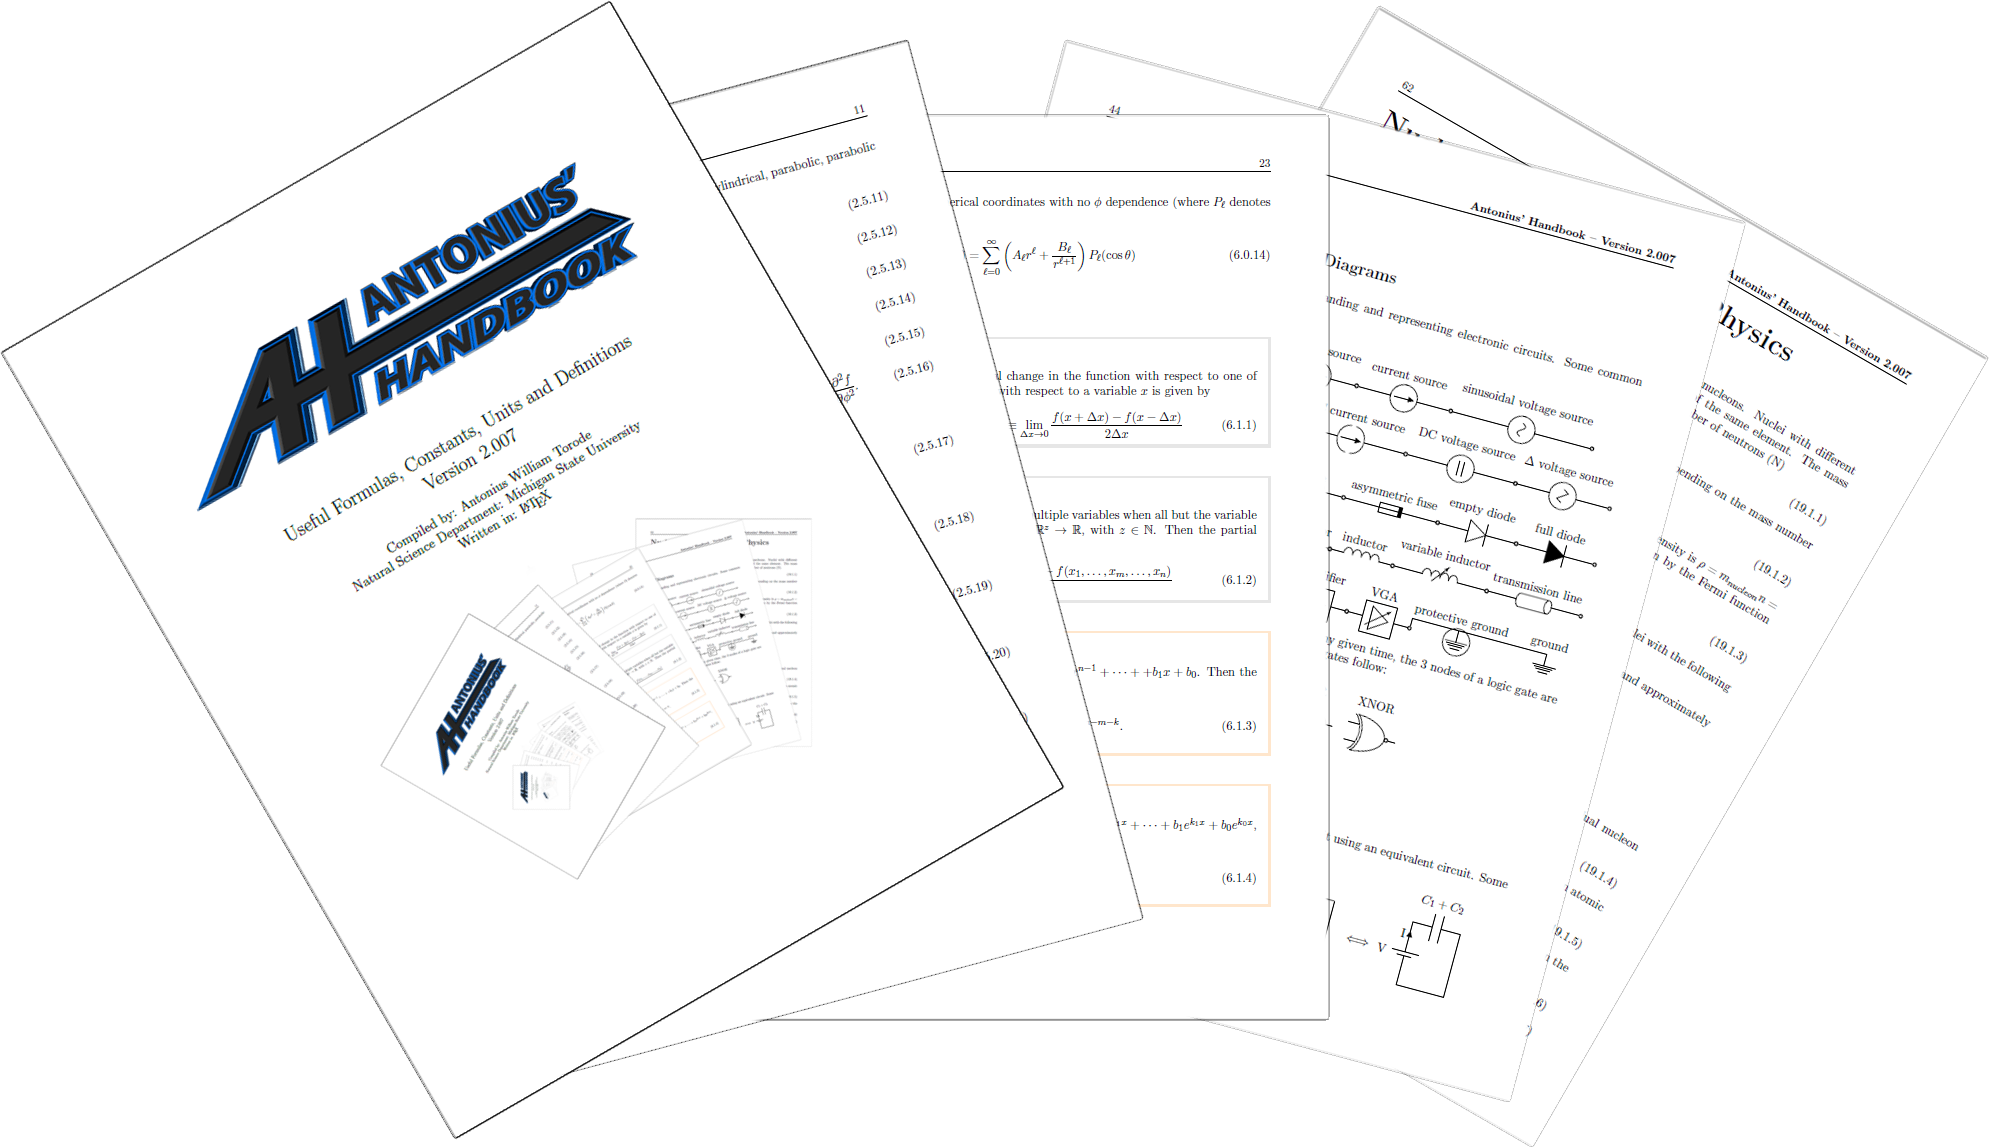
\includegraphics[scale=1.6]{./Images/Covers/background_tunnel.png}
\end{center}

%Copywrite page
\pagestyle{empty}
%% copyrightpage
\begingroup
\footnotesize
\parindent 0pt
\parskip \baselineskip
\textcopyright{} 2025 Antonius Torode \\
All rights reserved.

This work may be distributed and/or modified under the conditions of Antonius’ General Purpose License (AGPL).

The original maintainer of this work is: Antonius Torode.

The current maintainer of this work is: Antonius Torode.


Chief Editor: Antonius Torode

%\hfill\begin{minipage}{\textwidth-1cm}Other contributors:\end{minipage}

Published by Antonius Torode. 

Hosted at: https://torodean.github.io/

Github Repository: https://github.com/torodean/Antonius-Compendium

%\begin{center}
%\begin{tabular}{ll}
%First Personal Release (Version 0.000): & January 2016 \\
%First Public Release (Version 1.000): &  July 2016 \\
%Most Current Revision Date (Version \Version): & \today 
%\end{tabular}
%\end{center}

\vfill

Torode, A.\\
\hspace*{1em} Antonius' Compendium. \\
\hspace*{2em} Applied Research Laboratories -- \\
\hspace*{2em} \today \\
\hspace*{2em} Volume II. \\
\hspace*{2em} Version: \Version



\endgroup
\clearpage

%Preface page
\begin{center}
	\textbf{Preface}
\end{center}

This document is a compilation of ideas, scratch work, derivations, useful formulas, definitions, constants, and general information used for my own studies as a reference while furthering self education. These are my notes. It's purpose is to provide a complete 'compendium' per say of various ideas used often. All the material in this document was either directly copied from one of the references listed at the end or derived from scratch. On occasion \textit{typos may exist} due to human error but will be corrected when discovered.
	
The version number is updated every time the document is distributed, printed for distribution, or a major update is added. This ensures that there is no two copies with different information and similar version numbers. The latest update date is automatically set to the current date each time the document is edited. Please refrain from distributing this handbook without permission from the original author/compiler. This book is formatted for printing.

\begin{center}
	\textbf{Topics Covered In This Book}
\end{center}

\begin{multicols}{2}
\begin{itemize}
	\item Machine Learning
	\item Artificial Intelligence
	\item Modeling
	\item Psychology
\end{itemize} 
\end{multicols}

The information in this book is in no way limited to the topics listed above. They serve as a simple guideline to what you will find within this document. For more information about this book or details about how to obtain your own copy please visit:
\begin{center}
	https://torodean.github.io/
\end{center}

\begin{quotation}
``Scientific theories deal with concepts, not with reality. All theoretical results are derived from certain axioms by deductive logic. In physical sciences the theories are so formulated as to correspond in some useful sense to the real world, whatever that may mean. However, this correspondence is approximate, and the physical justification of all theoretical conclusions is based on some form of inductive reasoning.'' - Athanasios Papoulis (Probability, Random Variables, and Stochastic Processes book)
\end{quotation}

\begin{center}
	\textbf{Disclaimer}
\end{center}

This book contains formulas, definitions, and theorems that by nature are very precise. Due to this, some of the material in this book was taken directly from other sources such as but not limited to Wolfram Mathworld. This is only such in cases where a change in wording could cause ambiguities or loss of information quality.  Following this, all sources used are listed in the references section and cited when used.


%Begins blank page.
\thispagestyle{empty}
\newpage
\vspace*{\stretch{1}}
\begin{center}
	\textit{This page intentionally left blank.\\ (Yes, this is a contradiction.)}
\end{center}
\vspace*{\stretch{1}}

%Begins table of contents
\tableofcontents


%Begin the mainmatter.
\setlength{\parindent}{0pt}
\mainmatter
\pagestyle{fancy}
\chapter{Constants and units}
\thispagestyle{fancy}
\begin{fancybox}[Physical Constants]{}	
\begin{center}
	\begin{tabular}{   l  |  c  |  l  |  l  }
		Constant & Symbol & Value & Units \\
		\hline
		Speed of light in a vacuum& c $\equiv 1/\sqrt{\mu_0\epsilon_0}$ & $2.99792458 \times 10^8$ & m/s \\
		Elementary charge& e & $1.602176565(35)\times 10^{-19}$ & C\\
		Gravitational constant& G & $6.67384(80)\times 10^{-11}$ & m$^3$kg$^{-1}$s$^{-2}$\\
		Avagadro's number& $N_a$ & $6.02214129(27)\times 10^{23}$ & mol$\cdot s^{-1}$\\
		Planck constant & $h$ & $ 6.62606872(52) \times 10^{-34}$ & J$\cdot$s \\
		& & $4.135668 \times 10^{-15}$ & eV$\cdot$s \\
		& $hc$ & 1239.84 & eV$\cdot$nm \\
		Reduced planck constant& $\hbar \equiv h/2\pi$ & $1.05\times 10^-{34}$ & J$\cdot$s\\
		Permittivity of the vacuum & $\epsilon_0$ & $8.854\times 10^{-12}$ & C$^2$N$^{-1}$m$^{-2}$ \\
		Permeability of the vacuum & $\mu_0$ & $4\pi\times 10^{-7}$ & N/A$^{2}$ \\
		Permeability of the vacuum & $\mu_0$ & $4\pi\times 10^{-7}$ & N/A$^2$ \\
		Boltzmann constant & $k_B$ & $1.38064852\times 10^{-23}$ & J/K \\
				 & & $8.61733\times 10^{-5}$ & eV/K \\
		Stefan-Boltzmann constant & $\sigma_{\textrm{B}} \equiv \frac{\pi^2k_B^4}{60\hbar^3c^3}$ & $5.670367(13)\times 10^{-8}$ & W$\cdot$m$^{-2}$K$^{-4}$ \\
		Thomson cross-section & $\sigma_e$ & $6.652\times10^{-29}$ & $m^2$ \\
		The Bohr Magneton & $\mu_B \equiv \frac{e\hbar}{2m}$ & $5.788\times 10^{-5}$ & eV/T \\
		& & $9.274\times 10^{-24}$ & Am$^2$ \\
		Mass of an electron & $m_e$ & $9.10938291(40)\times 10^{-31}$ & kg\\
		&  & $510.9989$ & keV/$c^2$\\
		Mass of a proton& $m_p$ & $1.6726218 \times 10^{-27}$ & kg\\
		&  & 938.27203 & MeV/$c^2$\\
		Mass of a neutron& $m_n$   & $1.6749274 \times 10^{-27}$ & kg \\
		& & $939.56536$ & MeV/$c^2$	\\
		Unified amu & $u$ &  $1.660538782\times 10^{-27}$ & kg \\
		  &   &  931.494028 & MeV/c$^2$ 
	\end{tabular}
\end{center}
\end{fancybox}

\begin{fancybox}[Stellar Data]{}
	\begin{center}
		\begin{tabular}{c|c|c|c|c|c}
			Spectral Type & $T_{eff}$ (K) & $M/M_\odot$ & $L/L_\odot$ & $R/R_\odot$ & $V_{mag}$ \\
			\hline
			O5 & 44,500 & 60 & $7.9\times 10^5$ & 12 &-5.7 \\
			B5 & 15,400 & 5.9 & 830 & 3.9 & -1.2 \\
			A5 & 8,200 & 2.0 & 14 & 1.7 & 1.9 \\
			F5 & 6,440 & 1.4 & 3.2 & 1.3 & 3.4 \\
			G5 & 5,770 & 0.92 & 0.79 & 0.92 & 4.9 \\
			K5 & 4,350 & 0.67 & 0.15 & 0.72 & 6.7 \\
			M5 & 3,170 & 0.21 & 0.011 & 0.27 & 12.3 \\
		\end{tabular}
	\end{center}
\end{fancybox}



\newpage
\begin{fancybox}[Astronomical Constants]{1}
\begin{center}
\begin{tabular}{   l  |  c  |  l  |  l  }
Constant & Symbol & Value & Units \\
\hline
Mass of Earth& $M_\oplus$ & $5.974 \times 10^{24}$ & kg\\
Mass of Sun& $M_\odot$ &$1.989  \times 10^{30}$ & kg\\
Mass of Moon& $M_{\leftmoon}$ &$7.36 \times 10^{22}$&  kg\\
Equatorial radius of Earth& $R_\oplus$ & $6.378 \times 10^6$& m\\
Equatorial radius of Sun& $R_\odot$ &$6.6955 \times 10^8$ & m\\
Equatorial radius of Moon& $R_{\leftmoon}$ &$1.737 \times 10^{6}$ & m\\
Mean density of Earth &  & 5515  & kg$\cdot$m$^{-3}$  \\
Mean density of Sun &  & 1408  & kg$\cdot$m$^{-3}$ \\
Mean density of Moon  & & 3346  & kg$\cdot$m$^{-3}$ \\
Earth-Moon distance& &$3.84 \times 10^8$ & m\\
Earth-Sun distance& &$1.496 \times 10^{11}$ & m \\
Luminosity of Sun & $L_\odot$  & $3.839\times 10^{26}$  & W  \\
Effective temp. of Sun &   & 5778  & K  \\
Hubble constant & $H_0$  & $70\pm 5$  & km$\cdot$s$^{-1}$Mpc$^{-1}$  \\
Parsec& pc & 206264.81 & AU\\
&  & $3.0856776 \times 10^{16}$ & m\\
& & $3.2615638$ & ly \\
Astronomical Unit & AU & $1.496 \times 10^{11}$ & m \\
Light year& ly & $9.461 \times 10^{15}$ & m \\
1 year on Earth& yr & 365.25 & days \\
&  & $3.15576 \times 10^{7}$& s 
\end{tabular}
\end{center}
\end{fancybox}

\begin{fancybox}[Solar System]{}
	\begin{center}
		\begin{tabular}{   l  |  c  |  l  |  l  | l}
			Planet & Symbol & Mass (kg) & Radius (m) & Sun-Distance (km) \\
			\hline
			Mercury & \mercury & $3.285 \times 10^{23}$ & 2.44 $\times 10^{6}$ & $5.791 \times 10^{10}$ \\
			Venus & \venus & $4.867 \times 10^{24}$ & $6.052 \times 10^{6}$ & $1.082 \times 10^{11}$   \\
			Mars & \mars & $6.39 \times 10^{23}$ & $3.390 \times 10^{6}$ & $2.279 \times 10^{11}$ \\
			Jupiter& \jupiter &$1.898 \times 10^{27}$ & $3.83 \times 10^{11}$ & $7.785 \times 10^{11}$  \\
			Saturn & \saturn & $5.683 \times 10^{26}$ & $5.8232 \times 10^{7}$ & $1.429 \times 10^{12}$  \\
			Uranus & \uranus & $8.681 \times 10^{25}$ & $2.5362 \times 10^{7}$ & $2.871 \times 10^{12}$  \\
			Neptune & \neptune & $1.024 \times 10^{26}$ & $2.4622 \times 10^{7}$ & $4.498 \times 10^{12}$  \\
			Pluto & \pluto & $1.309 \times 10^{22}$ & $1.187 \times 10^6$ & $5.906 \times 10^{12}$ 
		\end{tabular}
	\end{center}
\end{fancybox}

\newpage
\begin{fancybox}[Unit conversions]{}
	The International System of Units (SI) defines seven units of measure as a basic set from which all other SI units can be derived. These are [length](m), [time](s), [mass](kg), [electric current] $\equiv$ [Ampere](A), [temperature](K), [luminous intensity](cd), [amount of substance](mol).
	\begin{center}
		\begin{tabular}{c|l|l}
			Unit Symbol & Unit & Equivalence \\
			\hline
			C & [Coulomb] & [Ampere][time] \\
			N & [Newton] & [mass][length][time]$^{-2}$ \\
			P & [Pascal]  & [mass][length]$^{-1}$[time]$^{-2}$ \\
			J & [Joule]  & [mass][length]$^{2}$[time]$^{-2}$ \\
			W & [Watt]  & [mass][length]$^{2}$[time]$^{-3}$ \\
			 & & [Ohm][Ampere]$^2$ \\
			 & & [Volt]$^2$[Ohm]$^{-1}$ \\
			V & [Volt]  & [mass][length]$^{2}$[time]$^{-3}$[Ampere]$^{-1}$ \\
			Wb & [Weber]  & [mass][length]$^{2}$[time]$^{-2}$[Ampere]$^{-1}$ \\
			T & [Tesla]  & [mass][time]$^{-2}$[Ampere]$^{-1}$ \\
			H & [henry]  & [mass][length]$^{2}$[time]$^{-2}$[Ampere]$^{-2}$ \\
			$\Omega$ & [Ohm]  & [mass][length]$^{2}$[time]$^{-3}$[Ampere]$^{-2}$ \\
			F & [Farad]  & [mass]$^{-1}$[length]$^{-2}$[time]$^{4}$[Ampere]$^{2}$ \\
			Hz & [Hertz]  & [time]$^{-1}$ 
		\end{tabular}
	\end{center}
\end{fancybox}


\begin{fancybox}[Number Sets ($i \equiv \sqrt{-1}$)]{}
	\begin{center}
		\begin{tabular}{c|l||c|l}
			Symbol &  Set  & Symbol & Set   \\
			\hline
			$\mathbb{R}$ & Real numbers & $\emptyset$ & \{\} \\
			$\mathbb{N}\equiv \mathbb{N}_1$ & \{1,2,3,4,\dots\} & $\mathbb{Z}$ & \{\dots,-2,1,0,1,2,\dots\} \\
			$\mathbb{Z}^+ \equiv \mathbb{N}_0$ & \{0,1,2,3,\dots\} & $\mathbb{Z}^-$ & \{0,-1,-2,-3,-4,\dots\} \\
			$\mathbb{C}$ & $\{x+iy | x,y \in \mathbb{R}\}$ & $\mathbb{Q}$ & $\{\frac{x}{y} | x,y \in \mathbb{Z}\}$ \\
			$\mathbb{I}$ & $\{ix|x\in \mathbb{R}\}$ & $\mathbb{U}$ & Universal Set \footnote{Definition: The set containing all objects or elements and of which all other sets are subsets.} \\
			$\mathbb{A}$ & Algebraic Numbers\footnote{Any number that is a solution to a polynomial equation with rational coefficients.} & $\mathbb{T}$ & Transcendental Numbers \footnote{Any number that is not an Algebraic Number.} 
		\end{tabular}
	\end{center}
\end{fancybox}

\begin{fancybox}[Mathematical Notation]{}
	\begin{center}
		\begin{tabular}{c|l||c|l||c|l}
			$\forall$ & For all & $\exists$ & There exists & $\because$ & Because\\ 
			$\in$ & Is an element of & $\notin$ & Is not an element of  & $\therefore$ & Therefore\\
			$\implies$ & Implies & $\Longleftrightarrow$ & Bi conditional & $\approx$ & Approximately\\
			$\longrightarrow$ & Mapped to & $\nsubseteq$ & Is not a subset of & $\ll$ & Much smaller than\\
			$\subset$& Is a subset of & $\subseteq$ & Is a subset or equal to  & $\gg$ & Much greater than\\
			$\propto$ & Is proportional to & $\equiv$ & Is equivalent to  & $\cup$/$\cap$ & Union/Intersection \\
			$\perp$ & Is perpendicular to & $\parallel$ & Is parallel to  & : or $|$ & Such that\\
		\end{tabular}
	\end{center}
\end{fancybox}


\setlength{\parindent}{25pt}

\newpage
\chapter{Geometry and Trigonometry}
\thispagestyle{fancy}

\keyword{Geometry} is a branch of mathematics that deals with the study of shapes, sizes, positions, and properties of space. It explores the relationships and properties of points, lines, angles, surfaces, and solids. In geometry, fundamental concepts include:

\begin{enumerate}
	\item \keyword{Points}: Basic building blocks with no size or dimensions. They are represented by dots and are used to define other geometric elements.
	\item \keyword{Lines}: Straight paths that extend infinitely in both directions. They are made up of an infinite number of points.
	\item \keyword{Angles}: The measure of the rotation between two intersecting lines, rays, or line segments.
	\item \keyword{Polygons}: Closed figures formed by connecting line segments to create shapes like triangles, quadrilaterals, pentagons, etc.
	\item \keyword{Circles}: A set of points equidistant from a central point, forming a closed curve.
	\item \keyword{Three-dimensional shapes}: Solids such as cubes, spheres, cylinders, pyramids, etc., with length, width, and height.
	\item Higher-dimensional shapes or objects: In addition to the traditional two-dimensional and three-dimensional shapes, geometry also explores mathematical constructs extended to higher dimensions. These higher dimensions go beyond our familiar three-dimensional space and introduce concepts like 4D, 5D, and higher-dimensional shapes. For example, in 4D space, there could be hypercubes, 4D spheres, and other intriguing structures. While challenging to visualize, these higher-dimensional geometries play a crucial role in theoretical mathematics and various scientific fields, offering unique insights into the nature of space and dimensions beyond our immediate perception.
\end{enumerate}

Geometry plays a significant role in various fields, including architecture, engineering, art, design, physics, and many other disciplines. It helps us understand the physical world and solve problems related to spatial relationships and measurements. Euclidean geometry, founded by the ancient Greek mathematician Euclid, is one of the most well-known and widely studied branches of geometry. However, there are also other types of geometries, such as non-Euclidean geometries, which explore different axioms and concepts, leading to intriguing and diverse mathematical systems.

\newpage
\chapter{General Mathematics}
\thispagestyle{fancy}

Mathematics is a systematic field of study that deals with numbers, quantities, shapes, and patterns. It is often regarded as the language of science, as it provides a framework for analyzing and understanding various phenomena in the natural and social world. Mathematics involves a wide range of topics, including arithmetic, algebra, geometry, calculus, statistics, and more. It is based on rigorous logical reasoning and uses symbols and formulas to represent relationships and solve problems. Mathematics plays a crucial role in various fields, such as physics, engineering, economics, computer science, and many other disciplines, making it an essential tool for advancing knowledge and technology.


\section{Summation}

\begin{defn}[Summation Notation \label{Summation Definition}]{1}
	A sum is the result of addition. The symbol $\sum$ is used to represent the addition of a series of values. Let $..., x_{a-1}, x_a, x_{a+1}, ... ,x_{b-1}, x_b, x_{b+1}, ...$ be a fixed series $\mathbb{S}$, where each term $x_i\in\mathbb{S}$, $b, a \in \mathbb{N}$ are index values. Then the sum of values in the series from $a$ to $b$ is given by
	\begin{align}
		\sum_{i=a}^{b} x_i = x_a +  x_{a+1} + ... + x_{b-1} + x_b
	\end{align}
	In the context of summing over all of the values of a series for some index $i$, it is often written in different ways which are typically equivalent.
	\begin{align}
		\sum_{i\in\mathbb{S}} x_i \equiv \sum_{i} x_i
	\end{align}
	If the number of terms in the summation is infinite then it is called an infinite series.
\end{defn}

\begin{defn}[Product Notation \label{Product Definition}]{1}
	A product is the result of multiplication. The symbol $\prod$ is used to represent the multiplication of a series of values. Let $..., x_{a-1}, x_a, x_{a+1}, ... ,x_{b-1}, x_b, x_{b+1}, ...$ be a fixed series $\mathbb{S}$, where each term $x_i\in\mathbb{S}$, $b, a \in \mathbb{N}$ are index values. Then the product of values in the series from $a$ to $b$ is given by
	\begin{align}
		\prod_{i=a}^{b} x_i = x_a \cdot  x_{a+1} \cdot ... \cdot x_{b-1} \cdot x_b
	\end{align}
	In the context of multiplying over all of the values of a series for some index $i$, it is often written in different ways which are typically equivalent.
	\begin{align}
		\prod_{i\in\mathbb{S}} x_i \equiv \prod_{i} x_i
	\end{align}
	If the number of terms in the summation is infinite then it is called an infinite series.
\end{defn}

%Consider a finite sum of values in a sequence $x$ from index $a$ to $b$. If we square this sum we would get
%
%\begin{align}
%	\bigg[\sum_{i=a}^{b} x_i\bigg]^2 &= (x_a +  x_{a+1} + ... + x_{b-1} + x_b)^2 \\
%	&= (x_a +  x_{a+1} + x_{a+2} + ... + x_{b-1} + x_b)(x_a +  x_{a+1} + x_{a+2} + ... + x_{b-1} + x_b) \\
%	&= \hspace{1cm} x_a^2 + 2x_ax_{a+1} + 2x_ax_{a+2} + \cdots + 2x_ax_b \nonumber\\
%	& \hspace{1cm}+ 2x_{a+1}x_{a} + x_{a+1}^2 + 2x_{a+1}x_{a+2} + \cdots + 2x_{a+1}x_b \nonumber\\
%	& \hspace{1cm}+ 2x_{a+2}x_{a} + 2x_{a+2}a_{a+1} + x_{a+2}^2 + \cdots + 2x_{a+2}x_b \nonumber\\
%	& \hspace{1.5cm} \vdots \nonumber\\
%	& \hspace{1cm}+ 2x_{b}x_{a} + 2x_{b}a_{a+1} + 2x_{b}x_{a+2} + \cdots + x_b^2	
%\end{align}
%
%From this, a pattern can be observed. There exists an $x_i^2$ term for each $i \in [a,b]$. There then exists a term $2x_ax_b$ for  all $a \neq b$. Therefore, we can write this as
%
%\begin{align}
%	\bigg[\sum_{i=a}^{b} x_i\bigg]^2 &= \sum_{i=a}^{b} x_i^2 + 2\sum_{i=a}^{b}\sum_{j=a}^{b} x_ix_j (1-\delta_{ij}),
%\end{align}
%where $\delta_{ij}$ is the Kronecker delta function.
%\begin{defn}[Kronecker Delta]
%	The \keyword{Kronecker delta} $\delta_{ij}$ is a discrete version of the delta function
%	\begin{align}
%		\delta_{ij} = \begin{cases}
%			1, & \text{if } i = j \\
%			0, & \text{if } i \neq j \\
%		\end{cases}  \implies 1-\delta_{ij} = \begin{cases}
%		0, & \text{if } i = j \\
%		1, & \text{if } i \neq j \\
%		\end{cases} \hspace{2cm}
%	\end{align}
%\end{defn}



















\section{Binomial Coefficients}

\begin{defn}[Binomial Coefficient \label{Binomial Coefficient Definition}]{1}
	The binomial coefficient, ${{n}\choose{k}}$, often denoted as "n choose k," is a mathematical concept used in combinatorics to represent the number of ways to choose k items from a set of n distinct items, regardless of the arrangement of the chosen elements. 	
	\begin{align}
		{{n}\choose{k}}&=\frac{n!}{(n-k)!k!}
	\end{align}
\end{defn}

To begin with, a useful idea is to sum each term of the binomial coefficient which will be used later. First, by definition of the binomial coefficient, we can write
\begin{align}
	{{n}\choose{k}}&=\frac{n!}{(n-k)!k!} \label{binomial-coefficient-defn}\\
	&=\frac{(n-1)!n}{(n-k)!k!}\\&
	=\frac{(n-1)!n-k(n-1)!+k(n-1)!}{(n-k)!k!}\\
	&=\frac{(n-1)!(n-k)}{(n-k)!k!}+\frac{k(n-1)!}{(n-k)!k!}\\
	&=\frac{(n-1)!}{(n-1-k)!k!}+\frac{(n-1)!}{(n-k)!(k-1)!}\\&={{n-1}\choose{k}}+{{n-1}\choose{k-1}} \label{n-1choosek+n-1choosek-1}\\
	&\equiv {{m}\choose{k}}+{{m}\choose{k-1}}, \textrm{ with }m=n-1.
\end{align} 

Observe for a moment that (\ref{n-1choosek+n-1choosek-1}) can be expanding even further. By the same process of going from (\ref{binomial-coefficient-defn}) to (\ref{n-1choosek+n-1choosek-1}), we can say
\begin{align}
	{{n-1}\choose{k-1}} = {{n-2}\choose{k-1}}+{{n-2}\choose{k-2}}.
\end{align}
Thus, (\ref{n-1choosek+n-1choosek-1}) becomes
\begin{align}
	{{n}\choose{k}}={{n-1}\choose{k}}+{{n-2}\choose{k-1}}+{{n-2}\choose{k-2}}.
\end{align}
If we continue this pattern, we can see that we can write the binomial coefficients as a sum of binomial coefficients with incrementally decreasing numerators (i.e n!, (n-1)!, (n-2)!,...). This gives
\begin{align}
	{{n}\choose{k}}&={{n-1}\choose{k}}+{{n-2}\choose{k-1}}+{{n-3}\choose{k-2}}+\cdots+{{1}\choose{k+2-n}}+{{0}\choose{k+1-n}} \\
	&=\sum_{i=1}^{n}{{n-i}\choose{k+1-i}} \\
	&=\sum_{i=0}^{n-1}{{n-1-i}\choose{k-i}}.
\end{align}
Note that we stop the above sequence when the numerator of our factorial sequence has reached zero. If we were to continue the sequence, we would end up having negative factorials in our numerator which would make evaluating the binomial coefficient at that term and the following terms difficult. However, if we happen to have a smaller $k$ than $n$, it may be such that we end up having negative $k$ numbers. This is ok for now, as it will lead to complex infinities in the denominator of our binomial coefficient expressions hence making those terms zero. This will be demonstrated later. Now, suppose we claim the following theorem. 

\begin{theo}[opt]{1}
	For all $n\in \mathbb{N}$,
\begin{align}
	\sum_{i=0}^{n}{{n}\choose{i}} =\sum_{i=0}^{n}\frac{n!}{(n-i)!i!}= 2^n.
\end{align}
\end{theo}

\begin{proof}
	We can then do a proof by induction to prove this is in fact true for all $n,k \in \mathbb{N}$. First, we can see checking the base cases hold as when $n=0$, we have $1=1$, when $n=1$, we have $2=2$, and when $n=3$ we have $4=4$. Next, let's assume for any $n=k$ that (1) holds true. Now, if we let $n=k+1$ we have from the left hand side of our expression,
\begin{align}
	\sum_{i=0}^{k+1}{{k+1}\choose{i}}&={{k+1}\choose{0}}+{{k+1}\choose{1}}+\cdots+{{k+1}\choose{k}}+{{k+1}\choose{k+1}} \\
	&={{k}\choose{0}}+{{k}\choose{-1}}+{{k}\choose{1}}+{{k}\choose{0}}+\cdots+{{k}\choose{k}}+{{k}\choose{k-1}}+{{k}\choose{k+1}}+{{k}\choose{k}}\\
	&=2{{k}\choose{0}}+2{{k}\choose{1}}+\cdots+2{{k}\choose{k-1}}+2{{k}\choose{k}}\\
	&=2\sum_{i=0}^{k}{{k}\choose{i}}\\
	&=2(2^k)\\
	&=2^{k+1}.
\end{align}
Therefore, we can see that for $n=k+1$ that equation (8) holds true, and thus we conclude by induction that (8) holds for all $n\in\mathbb{N}$.
\end{proof} 

Note that in the above proof, we made use of ${{k}\choose{k+1}}={{k}\choose{-1}}=0$. If we were to evaluate each of these using the definition of the binomial coefficient above we may notice a slight issue. Suppose we try to evaluate ${{n}\choose{-1}}$. Using the definition from (1), we would have
\begin{align}
	{{n}\choose{-1}}&=\frac{n!}{(n-(-1))!(-1)!}\\&=\frac{n!}{(n+1)!(-1)!} \\
	&=\frac{n!}{(n)!(n+1)(-1)!} \\
	&=\frac{1}{(n+1)(-1)!}.
\end{align}
From above, we have a negative factorial in the denominator of our expression. Since this is not easily determined as a positive integer factorial would be, we will need to expand this using the Gamma function. 

\begin{defn}[The Gamma function \label{The Gamma function Definition}]{1}
The gamma function is a mathematical function that generalizes the concept of a factorial to non-integer and complex numbers. It is denoted by the Greek letter "$\Gamma$" (gamma) and defined as
\begin{align}
	\Gamma(n)=(n-1)!\equiv\int_{0}^{\infty}t^{n-1}e^{-t}\dt.
\end{align}
\end{defn}

Using this gamma function with $n=0$ gives
\begin{align}
	\Gamma(0)&=\int_{0}^{\infty}t^{-1}e^{-t}\dt.
\end{align}
Since $\lim\limits_{t\rightarrow 0^+}t^{-1}e^{-t}=\infty$, we can say the integral under the curve from $0$ to $\infty$ will be divergent, and thus $\infty$. Therefore $\Gamma(0)\equiv\infty$. This allows us to write (18) as
\begin{align}
	\frac{1}{(n+1)(-1)!} = \frac{1}{(n+1)\Gamma(0)}=\lim\limits_{x\rightarrow \infty}\frac{1}{x}=0.
\end{align}
Thus, we can say that ${{n}\choose{-1}}=0$. Similarly, by the same process, if we have ${{n}\choose{n+1}}$ we get
\begin{align}
	{{n}\choose{n+1}}&=\frac{n!}{(n-(n+1))!(n+1)!}\\
	&=\frac{n!}{(-1)!(n)!(n+1)}\\
	&=\frac{1}{(-1)!(n+1)}\\
	&=0
\end{align}



\newpage
\chapter{Statistics and Probability}
\thispagestyle{fancy}

\keyword{Probability} is a fundamental concept in mathematics and statistics that measures the likelihood of an event occurring. It is represented as a value between 0 and 1, where 0 indicates the event is impossible, 1 denotes certainty, and values between 0 and 1 represent various degrees of likelihood. In simple terms, probability quantifies how probable or likely it is for an event to happen based on the total number of possible outcomes. It helps us make informed decisions, predict outcomes, and understand uncertainty in various real-world scenarios, such as games of chance, weather forecasts, and medical diagnoses. To understand probability on a mathematical level, some definitions of terminology is needed.

A \keyword{state} (or outcome) is particular condition that something is in at a specific time. A \keyword{system} is an activity, experiment, process, or model with states or outcomes that are typically subject to uncertainty. A \keyword{sample space} of an system is the set of all possible states of a system. An \keyword{event} (also may be referred to as a trial or measurement) is any subset or collection of states contained in the sample space of a system. An event is a \keyword{simple event} if it consists of exactly one state and a \keyword{compound event} if it consistst of more than one state.

\begin{defn}[Probability]{Probability}
An \keyword{probability} $p$ can be defined as the asymptotic frequency of a system in the state $s$ ($s \in \Omega$, where $\Omega$ is the sample space of the system) by the total number of occurrences of that state $N_s$ in the limit of an infinite number of events $N$.
    \begin{align}
        p(s) = \lim_{N\rightarrow\infty}\frac{N_s}{N} \\
	p(s) \in [0,1] \forall s \in \Omega
    \end{align}
For a system with $n$ states, the total probabilities of all states must normalize to one.
    \begin{align}
        \sum_{i=0}^{n}p(i) = \sum_{s \in \Omega}p(i) = \lim_{N\rightarrow\infty}\frac{1}{N}\sum_{i=0}^{n}N_i = 1
    \end{align}
A \keyword{Bayesian probability} is defined as a person's knowledge of the outcome of a trial, based on the evidence at their disposal - often accompanied by an associated error. A \keyword{model probability} is an assumption or guess for the probability given the possibility of an infinite number of trials.
\end{defn}

Some more useful concepts for modeling a system are the mean (average) and standard deviation. 

\begin{defn}[Mean \label{Mean Definition}]
	If $x_1, ..., x_N$ denotes N separate measurements of one quantity $x$, then we define the mean (or average) $\braket{x}$ as
	\begin{align}
		\braket{x} = \frac{1}{N}\sum_{i=1}^{N}x_i \label{mean equation}
	\end{align}
\end{defn}

\begin{defn}[Standard Deviation \label{Standard Deviation Definition}]
	If $x_1, ..., x_N$ denotes N separate measurements of one quantity $x$, then we define the standard deviation $\sigma_x$ as
	\begin{align}
		\sigma_x = \sqrt{\frac{1}{N-1}\sum_{i}(x_i-\braket{x})^2}
	\end{align}
\end{defn}

When dealing with \keyword{Bayesian probability}, there is typically an uncertainty associated with the measurements or functions.

\begin{defn}[Mean \label{Mean Definition}]
	Suppose $x_0, ..., x_N$ denotes N separate measurements with associated uncertainties $\delta x_0, ..., \delta x_N$. If the measured values are used to compute some function $q(x_0, ..., x_N)$ and the uncertainties in $x_0, ..., x_N$ are independent and random, then the uncertainty in $q$ is
	\begin{align}
		\delta q = \sqrt{\sum_{i=0}^{N}\bigg(\frac{\delta q}{\delta x_i} \delta x_i\bigg)^2}.
	\end{align}
 It will always be true that 
 	\begin{align}
		\delta q \leq \sum_{i=0}^{N}\abs{\frac{\delta q}{\delta x_i}} \delta x_i.
	\end{align}
\end{defn}

\begin{defn}[Uncertainty \label{Uncertainty}]
	If $x_1, ..., x_N$ denotes N separate measurements of one quantity $x$, then we define the standard deviation $\sigma_x$ as
	\begin{align}
		\sigma_x = \sqrt{\frac{1}{N-1}\sum_{i}(x_i-\braket{x})^2}
	\end{align}
\end{defn}


%\newpage
%\chapter{Abstract Algebra}
\thispagestyle{fancy}

Abstract algebra is a branch of mathematics focused on studying algebraic structures like groups, rings, fields, and modules. These structures generalize arithmetic and algebraic operations beyond the familiar realm of numbers, allowing for a deeper understanding of symmetry, structure, and operations in mathematics.



\newpage
\chapter{Linear Algebra}
\thispagestyle{fancy}

\keyword{Linear algebra} is a branch of mathematics that focuses on the study of vector spaces, linear transformations, and systems of linear equations. It provides a powerful framework for representing and solving problems involving linear relationships between variables. Key concepts in linear algebra include:

\begin{itemize}
	\item \keyword{Vectors}: Vectors are mathematical objects that represent magnitude and direction. They can be represented as ordered lists of numbers and are used to describe quantities with both magnitude and direction, such as velocity and force.
	
	\item \keyword{Vector Spaces}: A vector space is a set of vectors that satisfy certain properties under addition and scalar multiplication. It forms the foundation of linear algebra and allows for the study of linear combinations and transformations.
	
	\item \keyword{Matrices}: Matrices are rectangular arrays of numbers or elements, organized into rows and columns. They are used to represent linear transformations and to solve systems of linear equations.
	
	\item \keyword{Linear Transformations}: Linear transformations are functions that preserve the structure of vector spaces. They map vectors from one vector space to another while maintaining properties like linearity and preservation of the origin.
	
	\item \keyword{Eigenvalues} and \keyword{Eigenvectors}: In linear algebra, eigenvalues and eigenvectors are associated with linear transformations. Eigenvectors are special vectors that remain in the same direction after a linear transformation, and eigenvalues represent how much the eigenvectors are scaled during the transformation.
\end{itemize}

Linear algebra finds applications in various fields, including physics, computer graphics, engineering, data science, and economics. It plays a fundamental role in solving systems of linear equations, understanding linear transformations, and providing tools to analyze complex systems with multiple variables and interactions. Moreover, it forms the basis for more advanced mathematical concepts and techniques in areas like optimization, machine learning, and numerical analysis.



\section{Linear Systems}

\begin{defn}[Linear Combination]{defn:linear combination}
A \keyword{linear combination} of $x_0,..., x_n$ has the form 
\begin{align*}
a_0x_0 + a_1x_1 + a_2x_2 + \cdots + a_nx_n,
\end{align*}
where the numbers $a_0,..., a_n \in \R$ are the combination’s coefficients. A linear
equation in the variables $x_0,..., x_n$ has the form $a_0x_0 + a_1x_1 + a_2x_2 + \cdots +
a_nx_n = d$, where $d \in\R$ is the constant. An $n$-tuple $(s_0, s_1,..., s_n) \in\R^n$ is a solution of, or satisfies, that equation
if substituting the numbers $s_0,..., s_n$ for the variables gives a true statement: $a_0s_0 + a_1s_1 + · · · + a_ns_n = d$. A system of linear equations
\begin{align*}
a_{0,0}x_0 + a_{0,1}x_1 + ... + a_{0,n}x_n &= d_0 \\
a_{1,0}x_0 + a_{1,1}x_1 + ... + a_{1,n}x_n &= d_1 \\
a_{2,0}x_0 + a_{2,1}x_1 + ... + a_{2,n}x_n &= d_2 \\
&\vdots \\
a_{m,0}x_0 + a_{m,1}x_1 + ... + a_{2,n}x_n &= d_m
\end{align*}
has the solution $(s_0, s_1,..., s_n)$ if that n-tuple is a solution of all of the equations.
\end{defn}

\begin{theo}[Gauss's Method]{theo:gauss's method}
If a linear system is changed to another by one of the following operations, then the two systems have the same set of solutions.
\begin{enumerate}
	\item An equation is swapped with another.
	\item An equation has both sides multiplied by a non-zero constant.
	\item An equation is replaced by the sum of itself and a multiple of another.
\end{enumerate}
\end{theo}
\begin{proof}[Proof for theorem \ref{theo:gauss's method} item 1]
	The proof for this one is trivial. If we have a system of linear equations with a tuple that satisfies those equations, then by definition \ref{defn:linear combination}, all the equations hold true with that tuple. By swapping any of them, they will still hold true, and thus swapping them has no effect on the set of solutions.
\end{proof}
\begin{proof}[Proof for theorem \ref{theo:gauss's method} item 2]
	The proof for this one is also trivial. Consider a system of linear equations with a tuple $(s_0, s_1,..., s_n) \in\R^n$ that satisfies those solutions. Then by definition \ref{defn:linear combination}, for all $i\in\N$, we have a true statement $a_{i,0}x_0 + a_{i,1}x_1 + ... + a_{i,n}x_n = d_i$. Suppose we multiply both sides of this equation by some $p\in\R$, where $p \neq 0$. Then we have $p(a_{i,0}s_0 + a_{i,1}s_1 + ... + a_{i,n}s_n)= pd_i$. Since the tuple is a solution to the equation, there has to exist some $pd_i$ value to satisfies this equation call it $d'_i$ (the prime representing our new linear system), giving us $a'_{i,0}s_0 + a'_{i,1}s_1 + ... + a'_{i,n}s_n) = pd_i = d'_i$, where $a'_i$ are some new coefficients $pa_i$ that satisfy the equation and $d'_i$ is some new constant. Our tuple will satisfy this equation, and since none of the other equations changed, it will also satisfy them. Therefore, our solution satisfies this new linear system. Since the solution was arbitrary, this implies that all solutions are also satisfied.
\end{proof}
\begin{proof}[Proof for theorem \ref{theo:gauss's method} item 3]
	The proof for this one is also trivial. Consider a system of linear equations with a tuple $(s_0, s_1,..., s_n) \in\R^n$ that satisfies those solutions. Let $p \in \R$. Take two equations in the system $a_{i,0}x_0 + a_{i,1}x_1 + ... + a_{i,n}x_n = d_i$ and $a_{j,0}x_0 + a_{j,1}x_1 + ... + a_{j,n}x_n = d_j$. We can construct a new equation by adding the first to a multiple of the second, say $d_i + pd_j$. this gives $d_i + pd_j = a_{i,0}x_0 + a_{i,1}x_1 + ... + a_{i,n}x_n + p(a_{j,0}x_0 + a_{j,1}x_1 + ... + a_{j,n}x_n)$. Since our tuple is a solution to both of these equations, we know that the first term $d_i$ and the second term $pd_j$ (when our tuple is plugged into the variables) will satisfy the new expression. Thus, since this tuple is a solution to this equation, and since none of the other equations changed, it will also satisfy them. Therefore, our solution satisfies this new linear system. Since the solution was arbitrary, this implies that all solutions are also satisfied.
\end{proof}

\begin{defn}[Gaussian Operations]{defn:gaussian operations}
	The three operations from theorem \ref{theo:gauss's method} are called \keyword{Gaussian operations} (or elementary reduction operations, or row operations). They are swapping, multiplying by a scalar, and row combination.
\end{defn}


\begin{defn}[Echelon Form]{defn:echelon form}
	In a system of equations, the initial variable with a non-zero coefficient within each row is referred to as the leading variable for that row. A system is said to be in \keyword{echelon form} when every leading variable, except for the first row's leading variable, is positioned to the right of the leading variable in the row above it. Additionally, any rows containing coefficients of all zeros are situated at the bottom. 
\end{defn}


In an echelon form linear system the variables that are not leading are \keyword{free}. An example of echelon form follows. Consider the equations $x - 4y + 2z = -1$, $7z + 3y = 10$, and $3x + 7z = 10$. The echelon form of these is 
\begin{align}
1x - 4y + 2z &= -1 \\
0x+3y + 7z &= 10 \\
3x+0y+1z &= 2
\end{align}
I added coefficients to each term in order to better demonstrate how the variables `line up.' This form is analogous to representing data in matrix format. For these equations, a matrix representation would be written as

\begin{align}
\begin{bmatrix}
1 & -4 & 2 \\
0 & 3 & 7 \\
3 & 0 & 1
\end{bmatrix}
\begin{bmatrix}
x \\
y \\
z
\end{bmatrix}
=
\begin{bmatrix}
-1 \\
10 \\
2
\end{bmatrix} 
\hspace{1cm} \text{or} \hspace{1cm} 
\left(
\begin{array}{ccc|c}
1 & -4 & 2 & -1 \\
0 & 3 & 7 & 10\\
3 & 0 & 1 & 2
\end{array}
\right)
\end{align}



\begin{defn}[Matrix]{defn:matrix}
	An $m\times n$ matrix is a rectangular array of numbers with $m$ rows and $n$ columns (2-dimensional). Each number in the matrix is an entry which has an index in each dimension. A matrix is typically denoted with an upper case letter. A matrix is typically a 2-dimensional object but can be mathematically extended into higher dimensions. for example, a $3x5$ matrix with elements $a_{mn}$ is denoted
	\begin{align}
	A = 
	\begin{bmatrix}
	a_{11} & a_{12} & a_{13} & a_{14} & a_{15} \\
	a_{21} & a_{22} & a_{23} & a_{24} & a_{25} \\
	a_{31} & a_{32} & a_{33} & a_{34} & a_{35} \\
	\end{bmatrix}
	\end{align}
\end{defn}



\newpage
\chapter{Calculus}
\thispagestyle{fancy}

\keyword{Calculus} is a branch of mathematics that deals with the study of change and motion. It encompasses two main components: differentiation and integration.

\begin{itemize}
	\item \keyword{Differentiation}: This involves finding the rate at which a quantity changes with respect to another variable. The derivative is a fundamental concept in calculus, representing the instantaneous rate of change of a function at a particular point. It helps analyze the behavior of functions, such as finding slopes of curves, determining maximum and minimum points, and understanding the concept of velocity and acceleration.
	
	\item \keyword{Integration}: Integration is the reverse process of differentiation. It involves calculating the accumulation or total amount of a changing quantity over an interval. The integral of a function represents the area under the curve of the function over a given range. It is used to solve problems involving areas, volumes, and quantities related to accumulation, such as calculating total distance traveled from a velocity function or finding the area of a region bounded by a curve.
\end{itemize}

Calculus has numerous real-world applications, ranging from physics and engineering to economics and biology. It provides essential tools for understanding how things change, predicting behavior, and solving complex problems that involve continuous change and motion. Developed independently by Isaac Newton and Gottfried Wilhelm Leibniz in the 17th century, calculus remains a fundamental and powerful branch of mathematics used in various scientific and practical domains.









\section{Definitions and General Differential Equations}
 The derivative of a function represents an infinitesimal change in the function with respect to one of its variables \cite{bib:Wolfram}. 
\begin{defn}[Derivative]{defn:derivative} 
	Let $f:\mathbb{R}\rightarrow\mathbb{R}$. Then the derivative of $f$ with respect to a variable $x$ is given by
	\begin{align*}
	\frac{d}{dx}f(x)\equiv f'(x) \equiv\lim\limits_{\Delta x \rightarrow 0}\frac{f(x+\Delta x)-f(x)}{\Delta x} \equiv \lim\limits_{\Delta x \rightarrow 0}\frac{f(x+\Delta x)-f(x-\Delta x)}{2\Delta x}
	\end{align*}
\end{defn}
Similarly, partial derivatives are defined as derivatives of a function of multiple variables when all but the variable of interest are held fixed during the differentiation \cite{bib:Wolfram}. 
\begin{defn}[Partial Derivative]{defn:partial derivative}
	Let $f:\mathbb{R}^z\rightarrow\mathbb{R}$, with $z \in \mathbb{N}$. Then the partial derivative of $f$ with respect to a variable $x_m$ is given by
	\begin{align*}
	\frac{\partial}{\partial x_m}f(x_1,\dots,x_n) \equiv \lim\limits_{\Delta x \rightarrow 0}\frac{f(x_1,\dots,x_m+\Delta x, \dots,x_n)-f(x_1,\dots,x_m,\dots,x_n)}{\Delta x}
	\end{align*}
\end{defn}
A few rules from definition \ref{defn:derivative} can be defined.
\begin{theo}[Distributive Property Of Derivatives]{thm:derivative_distributive}
	Let $g:\mathbb{R}\rightarrow\mathbb{R}$, and $h:\mathbb{R}\rightarrow\mathbb{R}$ be continuous functions with $f(x)=g(x)+h(x)$. Then the derivative of $f$ with respect to the variable $x$ is 
	\begin{align*}
	\frac{d}{dx}f(x)=\frac{d}{dx}\big(g(x)+h(x)\big) = \frac{d}{dx}g(x)+\frac{d}{dx}g(x).
	\end{align*} 
\end{theo}

\begin{proof}[Proof for theorem \ref{thm:derivative_distributive}]
	Let $g:\mathbb{R}\rightarrow\mathbb{R}$, and $h:\mathbb{R}\rightarrow\mathbb{R}$ be continuous functions with $f(x)=g(x)+h(x)$. Then, by the definition of a derivative, we have
	\begin{align*}
	\frac{d}{dx}f(x)&=\lim\limits_{\Delta x \rightarrow 0}\frac{f(x+\Delta x)-f(x)}{\Delta x} \\
	&=\lim\limits_{\Delta x \rightarrow 0}\frac{(g+h)(x+\Delta x)-(g+h)(x)}{\Delta x} \\
	&=\lim\limits_{\Delta x \rightarrow 0}\frac{g(x+\Delta x)+h(x+\Delta x)-g(x)-h(x)}{\Delta x} \\
	&=\lim\limits_{\Delta x \rightarrow 0}\bigg(\frac{g(x+\Delta x)-g(x)}{\Delta x}+\frac{h(x+\Delta x)-h(x)}{\Delta x}\bigg) \\
	&=\lim\limits_{\Delta x \rightarrow 0}\frac{g(x+\Delta x)-g(x)}{\Delta x}+\lim\limits_{\Delta x \rightarrow 0}\frac{h(x+\Delta x)-h(x)}{\Delta x} \\
	&= \frac{d}{dx}g(x)+\frac{d}{dx}h(x).
	\end{align*}
	Thus, by simple manipulation we've shown
	\begin{align*}
	\frac{d}{dx}f(x)= \frac{d}{dx}g(x)+\frac{d}{dx}g(x).
	\end{align*}
\end{proof}
If we want to take the derivative of a function
Given a general polynomial function, we can give the following differentiation rule.
\begin{theo}[Polynomial Derivatives]{deriving_ordinary_polynomial}
	Let $f:\mathbb{R}\rightarrow\mathbb{R}$ be a function with $f(x)=c_nx^n+c_{n-1}x^{n-1}+\cdots++C_2x^2+c_1x+c_0$, where $c_n$ is constant for all $n$. Then
	\begin{align*}
	\frac{d}{dx}f(x)=f'(x)=nc_nx^{n-1}+(n-1)c_{n-1}x^{n-2}+\cdots+2c_2x+c_1
	\end{align*}
\end{theo}
\begin{proof}[Proof for theorem \ref{deriving_ordinary_polynomial}]
	Let $f:\mathbb{R}\rightarrow\mathbb{R}$ be a function with $f(x)=c_nx^n+c_{n-1}x^{n-1}+\cdots++C_2x^2+c_1x+c_0$, where $c_n$ is constant for all $n$. Let $g_n(x)=c_nx^n$. By theorem 1.1, we know that $f'(x)=g'_n(x)+g'_{n-1}(x)+\cdots+g_1(x)+g_0(x)$. Therefore, if we can prove $p(x)=Cx^n\implies p'(x)=nCx^n$, then this directly implies each term of $f(x)$ will have a derivative of equivalent form.
	Starting with $p$, we must first note that $p(x)=Cx^n$ and $p(x+h)=C(x+h)^n$. Inserting these into the limit definition will give us 
	\begin{align*}
	p'(x) = \lim_{h\to0} \frac{p(x+h)-p(x)}{h} = \lim_{h\to0} \frac{C(x+h)^n-Cx^n}{h}.
	\end{align*}
	As we can see, we can expand $(x+h)^n$ using the binomial theorem. This gives us
	\begin{align*}
	C\lim_{h\to0} \frac{\sum\limits_{k=0}^{n}{{n}\choose{k}}x^{n-k}h^k-x^n}{h}.
	\end{align*}
	If we denote $a_k={{n}\choose{k}}=\frac{n!}{k!(n-k)!}$, then expand the summation, we get
	\begin{align}
	C\lim_{h\to0}\frac{\sum\limits_{k=0}^{n}a_kx^{n-k}h^k-x^n}{h}=C\lim_{h\to0}\frac{a_0x^{n}+a_1x^{n-1}h+a_2x^{n-2}h^2+a_3x^{n-3}h^3+\dots+a_kx^{n-k}h^k-x^n}{h}.
	\end{align}
	If we determine $a_0$ and $a_1$ we get
	\begin{align}
	a_0 &=\frac{n!}{0!n!}=1 \\
	a_1 &=\frac{n!}{1!(n-1)!} =\frac{n!(n)}{(n-1)!(n)}=\frac{n!(n)}{n!}=n.
	\end{align}
	Inserting equations (1.2) and (1.3) into (1.1) yields
	\begin{align*}
	C\lim_{h\to0}\frac{x^n+nx^{n-1}h+a_2x^{n-2}h^2+a_3x^{n-3}h^3+\dots+a_kx^{n-k}h^k-x^n}{h}.
	\end{align*}
	Then, we see that the first and last terms add to zero
	\begin{align*}
	C\lim_{h\to0}\frac{nx^{n-1}h+a_2x^{n-2}h^2+a_3x^{n-3}h^3+\dots+a_kx^{n-k}h^k}{h}.
	\end{align*}
	From here, we simplify by dividing by $h$ and take the limit as $h \to 0$
	\begin{align*}
	C\lim_{h\to0}nx^{n-1}+a_2x^{n-2}h+a_3x^{n-3}h^2+\dots+a_kx^{n-k}h^{k-1}=Cnx^{n-1}.
	\end{align*}
	Hence, we have determined that $p'(x)=Cnx^{n-1}$ which directly implies
	\begin{align*}
	\frac{d}{dx}f(x)=f'(x)=nc_nx^{n-1}+(n-1)c_{n-1}x^{n-2}+\cdots+2c_2x+c_1
	\end{align*}
\end{proof}

Consider the basic product rule of a differential equation. The product rule is given by
\begin{theo}[Product Rule]{thm:product rule}
	Let $f:\mathbb{R}\rightarrow\mathbb{R}$ such that $f(x)$ and $g(x)$ are continuous functions of the variable $x$. We can then say
	\begin{align*}
		\frac{d}{dx}f(x)g(x)=g(x)\frac{d}{dx}f(x)+f(x)\frac{d}{dx}g(x)=f'(x)g(x)+f(x)g'(x)
	\end{align*}
\end{theo}
\begin{proof}[Proof for theorem \ref{thm:product rule}]
	Let $f:\mathbb{R}\rightarrow\mathbb{R}$ such that $f(x)$ and $g(x)$ are continuous functions of the variable $x$. By the definition of the derivative, we have
	\begin{align*}
		\frac{d}{dx}f(x)g(x)&=\lim\limits_{\Delta x \rightarrow 0}\frac{f(x+\Delta x)g(x+\Delta x)-f(x)g(x)}{\Delta x} \\
		&=\lim\limits_{\Delta x \rightarrow 0}\frac{f(x+\Delta x)g(x+\Delta x)-f(x+\Delta x)g(x)+f(x+\Delta x)g(x)-f(x)g(x)}{\Delta x} \\
		&=\lim\limits_{\Delta x \rightarrow 0}\frac{f(x+\Delta x)\big(g(x+\Delta x)-g(x)\big)+g(x)\big(f(x+\Delta x)-f(x)\big)}{\Delta x} \\
		&=\lim\limits_{\Delta x \rightarrow 0}f(x+\Delta x)\frac{g(x+\Delta x)-g(x)}{\Delta x}+\lim\limits_{\Delta x \rightarrow 0}g(x)\frac{f(x+\Delta x)-f(x)}{\Delta x} \\
		&=f(x)\frac{d}{dx}g(x)+g(x)\frac{d}{dx}f(x) \\&=f'(x)g(x)+f(x)g'(x).
	\end{align*}
\end{proof}
It is thus clear that given two continuous functions of $x$, say $f(x)$ and $g(x)$, the derivative follows as
\begin{align}
	\frac{d}{dx}f(x)g(x) &= g(x)\frac{d}{dx}f(x)+f(x)\frac{d}{dx}g(x) \\
 		             &= f(x)g'(x)+g(x)f'(x). \label{product_rule_n1}
\end{align}
Following this, the second derivative is given by
\begin{align}
	\frac{d^2}{dx^2}f(x)g(x)&=\frac{d}{dx}\bigg(g(x)\frac{d}{dx}f(x)\bigg)+\frac{d}{dx}\bigg(f(x)\frac{d}{dx}g(x)\bigg) \\
	&=\frac{d}{dx}f(x)\frac{d}{dx}g(x)+g(x)\frac{d^2}{dx^2}f(x)+f(x)\frac{d^2}{dx^2}g(x)+\frac{d}{dx}f(x)\frac{d}{dx}g(x) \\
	&=2\frac{d}{dx}f(x)\frac{d}{dx}g(x)+g(x)\frac{d^2}{dx^2}f(x)+f(x)\frac{d^2}{dx^2}g(x) \\
	&= f(x)g''(x)+2f'(x)g'(x)+f''(x)g(x). \label{product_rule_n2}
\end{align}
Similarly, the third derivative is given by
\begin{align}
	\frac{d^3}{dx^3}f(x)g(x)&=\frac{d}{dx}\bigg(2\frac{d}{dx}f(x)\frac{d}{dx}g(x)+g(x)\frac{d^2}{dx^2}f(x)+f(x)\frac{d^2}{dx^2}g(x)\bigg) \\
	&=\frac{d}{dx}\bigg(2\frac{d}{dx}f(x)\frac{d}{dx}g(x)\bigg)+\frac{d}{dx}\bigg(g(x)\frac{d^2}{dx^2}f(x)\bigg)+\frac{d}{dx}\bigg(f(x)\frac{d^2}{dx^2}g(x)\bigg).
\end{align}
This derivative can be done in parts to help keep track of what is being done. Let us denote each term in the above sum as $h_1(x)$, $h_2(x)$ and $h_3(x)$ respectively. Then we have
\begin{align}
	h_1(x)&= \frac{d}{dx}\bigg(2\frac{d}{dx}f(x)\frac{d}{dx}g(x)\bigg) \\
	h_2(x)&=\frac{d}{dx}\bigg(g(x)\frac{d^2}{dx^2}f(x)\bigg) \\
	h_3(x)&=\frac{d}{dx}\bigg(f(x)\frac{d^2}{dx^2}g(x)\bigg).
\end{align}
Simplifying these expressions then gives
\begin{align}
	h_1(x)&= \bigg(2\frac{d^2}{dx^2}f(x)\frac{d}{dx}g(x)+2\frac{d}{dx}f(x)\frac{d^2}{dx^2}g(x)\bigg) \\
	h_2(x)&=\bigg(\frac{d}{dx}g(x)\frac{d^2}{dx^2}f(x)+g(x)\frac{d^3}{dx^3}f(x)\bigg) \\
	h_3(x)&=\bigg(\frac{d}{dx}f(x)\frac{d^2}{dx^2}g(x)+f(x)\frac{d^3}{dx^3}g(x)\bigg).
\end{align}
Then, adding these three expressions together gives us
\begin{align}
	\frac{d^3}{dx^3}f(x)g(x)&=f(x)\frac{d^3}{dx^3}g(x)+3\frac{d}{dx}f(x)\frac{d^2}{dx^2}g(x)+3\frac{d^2}{dx^2}f(x)\frac{d}{dx}g(x)+g(x)\frac{d^3}{dx^3}f(x)\\
	&=f(x)g'''(x)+3f'(x)g''(x)+3f''(x)g'(x)+f'''(x)g(x). \label{product_rule_n3}
\end{align}
Using the product rule, a nice pattern seems to be emerging as we continually apply it to the same function. From equations (\ref{product_rule_n1}), (\ref{product_rule_n2}) and (\ref{product_rule_n3}), we can see that it appears to be a similar pattern as when applying the binomial expansion theorem. As a reminder, the binomial expansion theorem is
\begin{align}
	(a+b)^n&=\sum_{k=0}^{n}{{n}\choose{k}}a^{n-k}b^k \\
	{{n}\choose{k}}&= \frac{n!}{k!(n-k)!}.
\end{align}
If we observe the first three terms of this (with $n=1,2,3$), we have
\begin{align}
	(a+b)^1&=a+b\\
	(a+b)^2&= a^2+2ab+b^2 \\
	(a+b)^3 &= a^3+3a^2b+3ab^2+b^3.
\end{align}
Comparing this to the three equations in questions allows us to notice interesting similarities. If we expand this to $n$ we have
\begin{align}
	(a+b)^n=a^nb^0+{{n}\choose{1}}a^{n-1}y^1+\cdots+{{n}\choose{n-1}}ab^{k-1}+a^0b^k. \label{binomial_expansion_00}
\end{align}
Now, let $a=\frac{d}{dx}g(x)$ and $b=\frac{d}{dx}f(x)$. If we temporarily define\footnote{This is solely for an easy way of noticing the similarities in the formulas, these equations do not necessarily hold and are not used once the equations are expanded.} the following conditions
\begin{align}
	\bigg(\frac{d}{dx}h(x)\bigg)^n&:=\frac{d^n}{dx^n}h(x) \label{redefinition_derivative_00}\\
	\frac{d}{dx}g(x)+\frac{d}{dx}f(x) &:= \frac{d}{dx}g(x)f(x) \label{redefinition_derivative_01},
\end{align}
then inserting $a$ and $b$ into equation (\ref{binomial_expansion_00}) gives
\begin{align}
	\bigg[\frac{d}{dx}g(x)+\frac{d}{dx}f(x) \bigg]^n=\bigg(\frac{d}{dx}g(x)\bigg)^n\bigg(\frac{d}{dx}f(x)\bigg)^0+{{n}\choose{1}}\bigg(\frac{d}{dx}g(x)\bigg)^{n-1}\bigg(\frac{d}{dx}f(x)\bigg)^1+\cdots \\ \cdots+{{n}\choose{n-1}}\bigg(\frac{d}{dx}g(x)\bigg)\bigg(\frac{d}{dx}f(x)\bigg)^{n-1}+\bigg(\frac{d}{dx}g(x)\bigg)^0\bigg(\frac{d}{dx}f(x)\bigg)^n.
\end{align}
Simplifying the above expression gives us
\begin{align}
	\frac{d^n}{dx^n}g(x)f(x)=f(x)\frac{d^n}{dx^n}g(x)+{{n}\choose{1}}\frac{d^{n-1}}{dx^{n-1}}g(x)\frac{d}{dx}f(x)+\cdots \\
	\cdots+{{n}\choose{n-1}}\frac{d}{dx}g(x)\frac{d^{n-1}}{dx^{n-1}}f(x)+g(x)\frac{d^n}{dx^n}f(x).
\end{align}
Therefore, we can see that with our re-definitions in equations (\ref{redefinition_derivative_00}) and (\ref{redefinition_derivative_01}), it appears that the $n^{\textrm{th}}$ derivative of something using the product rule can be expressed using the binomial expansion theorem. At least to $n=3$ we can see from above that this is accurate. If we want to determine if this works for all values of $n$, we can try a proof by induction. Before going any further, since this may be a large amount of work for such a simple idea, let us quickly have a sanity check. We claim that the terms of the product rule can be expanded using the binomial theorem. It is important to note that when taking the product rule of an expression, you get two new expressions. Then, taking the product rule again will double those two into four, and then those four into eight, and so on. So we can see that each product rule doubles the number of terms we have. The binomial coefficient is used when we have like terms to combine them. If we were to add up each binomial coefficient in the sum, we should then see that each sum of coefficients is the same number of terms we would get as if we doubled our expression each time. If this were not so then our situation would have a flaw. In other words, it must hold true that
\begin{align}
	\sum_{i=0}^{n}{{n}\choose{k}} = 2^n.
\end{align}
This indeed is true. See theorem \ref{thm:Summing Over All binomial coefficients}. Now, we know from equations (\ref{product_rule_n1}), (\ref{product_rule_n2}) and (\ref{product_rule_n3}) that cases $n=1,2,3$ all hold. Next, if we assume that for any $n=k$ that
\begin{align}
	\frac{d^k}{dx^k}g(x)f(x)&=f(x)\frac{d^k}{dx^k}g(x)+{{k}\choose{1}}\frac{d^{k-1}}{dx^{k-1}}g(x)\frac{d}{dx}f(x)+\cdots \nonumber\\
	&\hspace{1cm}\cdots+{{k}\choose{k-1}}\frac{d}{dx}g(x)\frac{d^{k-1}}{dx^{k-1}}f(x)+g(x)\frac{d^k}{dx^k}f(x) \\
	&=\sum_{i=0}^{k}{{k}\choose{i}}\bigg[\frac{d^i}{dx^i}f(x) \bigg]\bigg[\frac{d^{k-i}}{dx^{k-i}}g(x) \bigg] \label{repeating_product_rule_final_k}
\end{align}
holds true, we can then determine if it holds true for $n=k+1$. This gives
\begin{align}
	\frac{d^{k+1}}{dx^{k+1}}g(x)f(x)&=f(x)\frac{d^{k+1}}{dx^{k+1}}g(x)+{{{k+1}}\choose{1}}\frac{d^{k}}{dx^{k}}g(x)\frac{d}{dx}f(x)+\cdots \nonumber\\
	&\hspace{1cm}\cdots+{{k+1}\choose{k}}\frac{d}{dx}g(x)\frac{d^{k}}{dx^{k}}f(x)+g(x)\frac{d^{k+1}}{dx^{k+1}}f(x) \\
	&=\sum_{i=0}^{k+1}{{k+1}\choose{i}}\bigg[\frac{d^i}{dx^i}f(x) \bigg]\bigg[\frac{d^{k+1-i}}{dx^{k+1-i}}g(x) \bigg].
\end{align}
If we were to manually evaluate the $n=k+1$ term of this expression we would have
\begin{align}
	\frac{d}{dx}\frac{d^{k}}{dx^{k}}g(x)f(x)= \frac{d}{dx}\sum_{i=0}^{k}{{k}\choose{i}}\bigg[\frac{d^i}{dx^i}f(x) \bigg]\bigg[\frac{d^{k-i}}{dx^{k-i}}g(x) \bigg].
\end{align}
Since differentiating is distributive (by theorem \ref{thm:derivative_distributive}), we can evaluate each term of this sum and compare it to (32) and (33). Doing this, we can use the product rule to first get
\begin{align}
	\frac{d^{k+1}}{dx^{k+1}}g(x)f(x)=\sum_{i=0}^{k}{{k}\choose{i}}\bigg[\frac{d^{i+1}}{dx^{i+1}}f(x) \bigg]\bigg[\frac{d^{k-i}}{dx^{k-i}}g(x) \bigg]+{{k}\choose{i}}\bigg[\frac{d^i}{dx^i}f(x) \bigg]\bigg[\frac{d^{k+1-i}}{dx^{k+1-i}}g(x) \bigg]. 
\end{align}
From here, writing out the series explicitly allows us to combine terms in a useful matter. This would obviously be tedious to write out so let us denote each term by $a_i$, for any $i^{\textrm{th}}$ term in the summation. Writing out a few of the terms then gives
\begin{align}
	a_0&={{k}\choose{0}}\bigg[\frac{d^{1}}{dx^{1}}f(x) \bigg]\bigg[\frac{d^{k}}{dx^{k}}g(x) \bigg]+{{k}\choose{0}}f(x)\bigg[\frac{d^{k+1}}{dx^{k+1}}g(x) \bigg] \\
	a_1&={{k}\choose{1}}\bigg[\frac{d^{2}}{dx^{2}}f(x) \bigg]\bigg[\frac{d^{k-1}}{dx^{k-1}}g(x) \bigg]+{{k}\choose{1}}\bigg[\frac{d}{dx}f(x) \bigg]\bigg[\frac{d^{k}}{dx^{k}}g(x) \bigg] \\
	a_2&={{k}\choose{2}}\bigg[\frac{d^{3}}{dx^{3}}f(x) \bigg]\bigg[\frac{d^{k-2}}{dx^{k-2}}g(x) \bigg]+{{k}\choose{2}}\bigg[\frac{d^2}{dx^2}f(x) \bigg]\bigg[\frac{d^{k-1}}{dx^{k-1}}g(x) \bigg]\\
	&\vdots \nonumber\\
	a_{k-2}&={{k}\choose{k-2}}\bigg[\frac{d^{k-1}}{dx^{k-1}}f(x) \bigg]\bigg[\frac{d^{2}}{dx^{2}}g(x) \bigg]+{{k}\choose{k-2}}\bigg[\frac{d^{k-2}}{dx^{k-2}}f(x) \bigg]\bigg[\frac{d^{3}}{dx^{3}}g(x) \bigg]\\
	a_{k-1}&={{k}\choose{k-1}}\bigg[\frac{d^{k}}{dx^{k}}f(x) \bigg]\bigg[\frac{d}{dx}g(x) \bigg]+{{k}\choose{v}}\bigg[\frac{d^{k-1}}{dx^{k-1}}f(x) \bigg]\bigg[\frac{d^{2}}{dx^{2}}g(x) \bigg]\\
	a_k&={{k}\choose{k}}\bigg[\frac{d^{k+1}}{dx^{k+1}}f(x) \bigg]g(x)+{{k}\choose{k}}\bigg[\frac{d^k}{dx^k}f(x) \bigg]\bigg[\frac{d}{dx}g(x) \bigg].
\end{align}
At this point, it becomes obvious as to why the $f^{(n)}(x)$ notation of a derivative was invented, and switching over will greatly help in our next step. Changing our notation gives us 
\begin{align}
	a_0&={{k}\choose{0}}f^{(1)}(x) g^{(k)}(x)+{{k}\choose{0}}f(x)g^{(k+1)}(x) \label{repeating_product_rule_a0}\\
	a_1&={{k}\choose{1}}f^{(2)}(x) g^{(k-1)}(x) +{{k}\choose{1}}f^{(1)}(x) g^{(k)}(x) \\
	a_2&={{k}\choose{2}}f^{(3)}(x) g^{(k-2)}(x) +{{k}\choose{2}}f^{(2)}(x) g^{(k-1)}(x) \\
	&\vdots \nonumber\\
	a_{k-2}&={{k}\choose{k-2}}f^{(k-1)}(x) g^{(2)}(x) +{{k}\choose{k-2}}f^{(k-2)}(x) g^{(3)}(x)\\
	a_{k-1}&={{k}\choose{k-1}}f^{(k)}(x) g^{(1)}(x)+{{k}\choose{k-1}}f^{(k-1)}(x) g^{(2)}(x)\\
	a_k&={{k}\choose{k}}f^{(k+1)}(x) g(x)+{{k}\choose{k}}f^{(k)}(x)g^{(1)}(x). \label{repeating_product_rule_ak}
\end{align}
Our end goal is to get this expression to be in the same form as in equation (\ref{repeating_product_rule_final_k}). If we first re-write equation (\ref{repeating_product_rule_final_k}) using $f^{(n)}(x)$ notation, we can easily see what our end goal is. This is
\begin{align}
	\sum_{i=0}^{k+1}{{k+1}\choose{i}}f^{(i)}(x) g^{(k+1-i)}(x) \label{repeating_product_rule_final}.
\end{align}
The next step is then summing expressions (\ref{repeating_product_rule_a0}) through (\ref{repeating_product_rule_ak}), then determining if what we get is equivalent to equation (\ref{repeating_product_rule_final}). Let $\Upsilon=a_0+a_1+\cdots+a_{k-1}+a_k$, then we have
\begin{align}
	\Upsilon&={{k}\choose{0}}f(x)g^{(k+1)}(x)+{{k}\choose{0}}f^{(1)}(x)g^{(k)}(x)+{{k}\choose{1}}f^{(1)}(x)g^{(k)}(x)+\cdots \nonumber\\
	&\hspace{1cm}\cdots+{{k}\choose{k}}f^{(k)}(x)g^{(1)}(x)+{{k}\choose{k-1}}f^{(k)}(x)g^{(1)}(x)+{{k}\choose{k}}f^{(k+1)}(x)g(x) \\
	&={{k}\choose{0}}f(x)g^{(k+1)}(x)+\bigg[{{k}\choose{0}}+{{k}\choose{1}} \bigg]f^{(1)}(x)g^{(k)}(x)+\cdots \nonumber\\
	&\hspace{1cm}\cdots+\bigg[{{k}\choose{k-1}}+{{k}\choose{k}} \bigg]f^{(k)}(x)g^{(1)}(x)+{{k}\choose{k}}f^{(k+1)}(x)g(x)\\
	&=\sum_{i=0}^{k+1}\bigg[{{k}\choose{i-1}}+{{k}\choose{i}} \bigg]f^{(i)}(x)g^{(k+1-i)}(x). \label{repeating_product_rule_00}
\end{align}
Using the definition of the binomial coefficient and the derivation in (7), if we let $k=m-1 \implies m=k+1$, we can re-write the binomial coefficient in equation (\ref{repeating_product_rule_00}) as follows.
\begin{align}
	{{k}\choose{i-1}}+{{k}\choose{i}}={{m-1}\choose{i-1}}+{{m-1}\choose{i}}={{m}\choose{i}}={{k+1}\choose{i}}.
\end{align}
Thus, equation (\ref{repeating_product_rule_00}) becomes
\begin{align}
	\Upsilon=\sum_{i=0}^{k+1}{{k+1}\choose{i}}f^{(i)}(x)g^{(k+1-i)}(x).
\end{align}
Now, $\Upsilon=a_0+a_1+\cdots+a_{k-1}+a_k=(35)$ which we have shown is equivalent to equation (\ref{repeating_product_rule_00}). Therefore, we can conclude that (28) holds for all $n\in\mathbb{N}$, which allows us to tidy our work up as a theorem.
\begin{theo}[Repeating Product Rule]{thm:repeating product rule}
	Let $f:\mathbb{R}\rightarrow\mathbb{R}$ and $g:\mathbb{R}\rightarrow\mathbb{R}$ be continuous and differentiable functions of the variable $x$. Then the $m^{\textrm{th}}$ derivative of $f(x)g(x)$ with respect to $x$ is
	\begin{align*}
		\frac{d^m}{dx^m}f(x)g(x)=\sum_{i=0}^{n}{{n}\choose{i}}\bigg[\frac{d^i}{dx^i}f(x) \bigg]\bigg[\frac{d^{n-i}}{dx^{n-i}}g(x) \bigg].
	\end{align*}
\end{theo}



Consider a division of two functions rather than multiplication. The product rule can be used to derive what is referred to as the \keyword{quotient rule}. Begin by taking two arbitrary functions that are continuous and differentiable $f(x)$ and $g(x)$. What we want to find is $\frac{d}{dx} \frac{f(x)}{g(x)}$. We begin by applying the product rule from theorem \ref{thm:product rule}, which gives
\begin{align}
	\frac{d}{dx} \frac{f(x)}{g(x)} = f(x)\left[\frac{d}{dx} \frac{1}{g(x)}\right] + \frac{1}{g(x)}\left[\frac{d}{dx} f(x)\right] \label{quotient_rule_00}.
\end{align}
Let $u(x)=\frac{1}{g(x)}$. We want to determine $u'(x)$ in order to simplify equation (\ref{quotient_rule_00}). From the definition of $u(x)$, we can then say $u(x)g(x)=1$. The derivative of a constant value is just zero, so if we differentiate both sides (by yet again applying the product rule from theorem \ref{thm:product rule}), we get
\begin{align}
	\frac{d}{dx}u(x)g(x)=\frac{d}{dx}1 \implies u(x)g'(x) + u'(x)g(x)=0.
\end{align}
Solving this for $u'(x)$ gives us $\frac{d}{dx} \frac{1}{g(x)}$ which we is then equal to 
\begin{align}
	u'(x) = \frac{d}{dx} u(x) = \frac{d}{dx} \frac{1}{g(x)} = \frac{-u(x)g'(x)}{g(x)} = -\frac{g'(x)}{g(x)^2} \label{quotient_rule_01}.
\end{align}
By taking equation (\ref{quotient_rule_01}) and substituting it into equation (\ref{quotient_rule_00}), we get
\begin{align}
	\frac{d}{dx} \frac{f(x)}{g(x)} = f(x)\left[-\frac{g'(x)}{g(x)^2}\right] + \frac{1}{g(x)}f'(x) = -\frac{f(x)g'(x)}{g(x)^2}+ \frac{g(x)f'(x)}{g(x)^2} = \frac{f'(x)g(x)-f(x)g'(x)}{g(x)^2}.
\end{align}

\begin{theo}[Quotient Rule]{thm:quotient rule}
	Let $f:\R \to \R$ and $g: \R\to\R$ be continuous and differentiable functions of the variable $x$. Then the derivative of $\frac{f(x)}{g(x)}$ with respect to $x$ is
	\begin{align}
		\frac{d}{dx} \frac{f(x)}{g(x)} = \frac{f'(x)g(x)-f(x)g'(x)}{g(x)^2}.
	\end{align}
\end{theo}
A special case of this quotient rule is when the numerator is $1$. This can be seen in equation (\ref{quotient_rule_00}). For simplicity, I will drop the "$(x)$" and assume functions with a single variable here. Taking consecutive derivatives of this give
\begin{align}
	\frac{d}{dx}\frac{1}{g} &= \frac{-g'}{g^2} \label{d/dx 1/g 1}\\
	\frac{d^2}{dx^2}\frac{1}{g} &= \frac{d}{dx}\frac{-g'}{g^2} = -\frac{d}{dx}g'\frac{1}{g^2} = -\frac{g''}{g^2}-g'\left(\frac{-2gg'}{g^4}\right) = -\frac{g''}{g^2}+\frac{2g'^2}{g^3} \label{d/dx 1/g 2}\\
	\frac{d^3}{dx^3}\frac{1}{g} &= \frac{d}{dx}\left(-\frac{g''}{g^2}+\frac{2g'^2}{g^3}\right) =- \frac{g'''}{g^2} - g''\frac{d}{dx}\frac{1}{g^2} +  \frac{4g'g''}{g^3} + 2g'^2\frac{d}{dx}\frac{1}{g^3}  \nonumber \\&= -\frac{g'''}{g^2}-g''\left(\frac{-2gg'}{g^4}\right)+\frac{4g'g''}{g^3}+2g'^2\left(\frac{-3g^2g'}{g^6}\right) \nonumber\\
	&= -\frac{g'''}{g^2}+\frac{2g'g''}{g^3}+\frac{4g'g''}{g^3}-\frac{6g'^3}{g^4} \nonumber\\
	&=\frac{6g'g''}{g^3}-\frac{6g'^3}{g^4}-\frac{g'''}{g^2} \label{d/dx 1/g 3}\\
	\frac{d^4}{dx^4}\frac{1}{g} &= \frac{d}{dx}\left(\frac{6g'g''}{g^3}-\frac{6g'^3}{g^4}-\frac{g'''}{g^2}\right) \nonumber \\
	&= 6g'g''\frac{d}{dx}\frac{1}{g^3}+\frac{1}{g^3}\frac{d}{dx}6g'g''-6g'^3\frac{d}{dx}\frac{1}{g^4}-\frac{1}{g^4}\frac{d}{dx}6g'^3-g'''\frac{d}{dx}\frac{1}{g^2}-\frac{1}{g^2}\frac{d}{dx}g'''\nonumber \\
	&= \frac{-18g'^2g''}{g^4}+\frac{6g'g'''+6g''^2}{g^3}+\frac{24g'^4}{g^5}-\frac{18g'^2g''}{g^4}+\frac{2g'g'''}{g^3}-\frac{g^{(4)}}{g^2}\nonumber \\
	&= \frac{-36g'^2g''}{g^4}+\frac{8g'g'''}{g^3}+\frac{6g''^2}{g^3}+\frac{24g'^4}{g^5}-\frac{g''''}{g^2} \label{d/dx 1/g 4}\\
	\frac{d^5}{dx^5}\frac{1}{g} &= \frac{-g^{(5)}}{g^2}-\frac{120g'^5}{g^6}+\frac{10g^{(4)}g'}{g^3}+\frac{20g'''g''}{g^3}-\frac{60g'''g'^2}{g^4}+\frac{240g'^3g''}{g^5}-\frac{90g'g''^2}{g^4},\label{d/dx 1/g 5}
\end{align}
and so on. Notice on that last one I spared the algebra. to find a pattern in this sequence, a few things can be noted. First. The factor of $\left(\frac{1}{g}\right)^m$ is common in every term. The maximum $m$ value here appears to be equal to $m=n+1$, where $n$ is the number of derivatives performed. There also seem to be at least one term for each $m$ value except for $m=1$ (for example, in equation (\ref{d/dx 1/g 1}) there is only a $g^2$ term, with a maximum $m=2$, but in equation (\ref{d/dx 1/g 5}), there are $m=2,3,4,5,\text{ and }6$ terms). Next, there is a common occurrence of $\frac{d^k}{dx^k}g$ terms, where the highest $k$ value appears to be $k=n$ in each derivative. There does not seem to be an immediate pattern with the coefficients. For each $\frac{d^n}{dx^n}$, there is also a $-\frac{g^{(n)}}{g^2}$ term.

Using these observations, we can begin to construct a potential formula to represent this pattern. It must be a sum of some kind, since it has summed terms. It must contain one term for each $\left(\frac{1}{g}\right)^m$ for all $1\leq m \leq n+1$. Each term will have some coefficient, which will likely be dependent on $m$, $n$, or both $m$ and $n$. And each term will have some product of $g^{(i)}$ terms. We can thus guess our formula to look something like
\begin{align}
	\frac{d^n}{dx^n}\frac{1}{g} \overset{?}{=} \sum_{m=0}^{n}\frac{C(n,m)}{g^{m+1}}G( g^{(i)}|i \leq n \in \N^+), \label{d/dx 1/g guess 00}
\end{align}
where $C(n,m)$ is some coefficient function dependent on $n$ and $m$, and $G(g^{(i)}|i \leq n \in \N^+) \equiv G(g^{(1)}, g^{(2)},...,g^{(n)})$ is some function which is a product of the repeated derivatives of $g(x)$ in some combination. Some possible steps to determine this formula better would of course be to then determine $G$ and $C$. We know the above equations involve deriving $g(x)$. With a careful and lucky observation, $G$ can be determined. Consider this derivative for a moment $\frac{d}{dx} g(x) =  g'(x)$. If we take consecutive derivatives, we simply get $\frac{d^i}{dx^i} g(x) =  g^{(i)}(x)$. Now consider this derivative for a moment $\frac{d}{dx} g(x)^2 =  2g(x)g'(x)$. When there are multiple terms of our function, the consecutive derivatives require the product rule, which would give $\frac{d^2}{dx^2} g(x)^2 =  2g(x)g''(x)+2g'(x)^2$. Careful observation will reveal that this corresponds to the derivatives in equation (\ref{d/dx 1/g 2}), where as the first derivative of $g(x)$ corresponds to the coefficients in equation (\ref{d/dx 1/g 1}). Taking a third derivative of $g(x)^2$ gives $\frac{d^3}{dx^3} g(x)^2 =  2g(x)g'''(x)+6g'(x)g''(x)$. This only closely correlates to equation (\ref{d/dx 1/g 3}). If instead we take the third derivative of $g(x)^3$, we have $\frac{d^3}{dx^3} g(x)^3 =  3(g(x)^2g'''(x)+2g'(x)^3 +6g'(x)g''(x)$, which indeed correlates to the coefficients in equation (\ref{d/dx 1/g 3}). This pattern appears to repeat. The excess $g$ terms in these will interfere with our $g^{m+1}$ denominator in equation (\ref{d/dx 1/g guess 00}), and so we should modify this to be some function, say $q(x, n, m)$ (It has a dependency on $m$ and $n$ because it's value may depend on which term in the summation it is), and determine if it needs to be changed. The pattern of $G$ reveals we can potentially make $G$ a function of $n$ (and more technically $n$ and $x$ since $g$ is a function of $x$) to get our correct factors of $g^{(i)}$ in each term.
\begin{align}
	G( g^{(i)}|i \leq n \in \N^+) \overset{?}{\equiv} G(n, x) \overset{?}{=} \frac{\partial^n}{\partial x^n}g(x)^n.
\end{align}
Inserting this into equation (\ref{d/dx 1/g guess 00}) gives
\begin{align}
	\frac{d^n}{dx^n}\frac{1}{g} \overset{?}{=} \sum_{m=0}^{n}\frac{C(n,m)}{q(x, n, m)}\frac{\partial^n}{\partial x^n}g(x)^n \label{d/dx 1/g guess 01}.
\end{align}
To determine $q$, we can write out the first few expansions of $G$.
\begin{align}
	\frac{d}{dx} g(x) &= g'(x) \label{d/dx g}\\
	\frac{d^2}{dx^2} g(x)^2 &=  2g(x)g''(x)+2g'(x)^2 \label{d^2/dx^2 g^2}\\
	\frac{d^3}{dx^3} g(x)^3 &= 3(g(x)^2g'''(x)+2g'(x)^3 +6g'(x)g''(x) \label{d^3/dx^3 g^3}\\
	\frac{d^4}{dx^4} g(x)^4 &= 4(6g'(x)^4+g(x)^3g^{(4)}(x)+9g(x)^2g''(x)^2+ 12g(x)^2g'(x)g^{(3)}(x)+36g(x)g'(x)^2g''(x)) \label{d^4/dx^4 g^4}
\end{align}
Using this and beginning with $n=1$, we have
\begin{align}
		\frac{d}{dx}\frac{1}{g} = \sum_{m=0}^{1}\frac{C(1,m)}{q(x, 1, m)}\frac{\partial}{\partial x}g(x) = \frac{C(1,0)}{q(x, 1, 0)}g'(x) + \frac{C(1,1)}{q(x, 1, 1)}g'(x).
\end{align}
We can let $C(1,0)=0$, which makes the first term vanish, $q(x,1,1) = g^{2}$, and $C(1,1) = -1$. For $n=2$ we have
\begin{align}
	\frac{d^2}{dx^2}\frac{1}{g} &\overset{?}{=} \sum_{m=0}^{2}\frac{C(2,m)}{q(x, 2, m)}\frac{\partial^2}{\partial^2 x}g(x)^2 \\ 
	&= \left[\frac{C(2,0)}{q(x, 2, 0)} + \frac{C(2,1)}{q(x, 2, 1)} + \frac{C(2,m)}{q(x, 2, 2)}\right]\left(2g(x)g''(x)+2g'(x)^2\right) \\
	&= \frac{C(2,0)}{q(x, 2, 0)}\left(2gg''+2g'^2\right) + \frac{C(2,1)}{q(x, 2, 2)}\left(2gg''(x)+2g'^2\right) + \frac{C(2,m)}{q(x, 2, 2)}\left(2gg''+2g'^2\right).
\end{align}
From this we can compare coefficients to equation \ref{d/dx 1/g 2} and thus we have
\begin{align}
	2g\left[\frac{C(2,0)}{q(x, 2, 0)}+ \frac{C(2,1)}{q(x, 2, 1)} + \frac{C(2,2)}{q(x, 2, 2)}\right] &= \frac{-1}{g^2} \\	
	2\left[\frac{C(2,0)}{q(x, 2, 0)}+ \frac{C(2,1)}{q(x, 2, 1)} + \frac{C(2,2)}{q(x, 2, 2)}\right] &= \frac{2}{g^3}
\end{align}
We can again make the first $m=0$ term have a zero constant ($C(2,0=0$)) causing it to vanish, then these become 
\begin{align}
	\frac{C(2,1)}{q(x, 2, 1)} + \frac{C(2,2)}{q(x, 2, 2)} &= \frac{-1}{2g^3} \\	
	\frac{C(2,1)}{q(x, 2, 1)} + \frac{C(2,2)}{q(x, 2, 2)} &= \frac{1}{g^3}
\end{align}
From this, $q(x,2,m)=\frac{1}{g^3}$, $C(2,1)+C(2,2) = \frac{-1}{2}$ and $C(2,1) + C(2,2) = 1$. \textcolor{red}{This cannot be true and is in fact a contradiction. Therefore we must conclude that equation (\ref{d/dx 1/g guess 01}) is incorrect!}. One thing of noteworthiness is that in the above process, if the steps were repeated for more $n$ values, there would always be each set of equations with the same coefficients leading to this contradiction. This is because $G$ did not depend on anything other than $n$ giving the same factor for each term of the sum. To remedy this, we can add an $m$ dependence to $G$ and allow the coefficient variables to cancel out the un-used terms. As long as we have the maximum $n$ value, we will have some equation that gives the correct $g^{(i)}$ terms and then we can make the other unwanted terms cancel. Thus, we can try to modify $G$ such that $G = \frac{\partial^n}{\partial x^n}g(x)^m$. This gives
\begin{align}
	\frac{d^n}{dx^n}\frac{1}{g} \overset{?}{=} \sum_{m=0}^{n}\frac{C(n,m)}{q(x, n, m)}\frac{\partial^n}{\partial x^n}g(x)^m \label{d/dx 1/g guess 02}.
\end{align}
We then try the same process again. Let $n=1$. We have
\begin{align}
	\frac{d}{dx}\frac{1}{g} = \sum_{m=0}^{1}\frac{C(1,m)}{q(x, 1, m)}\frac{\partial}{\partial x}g(x)^m =\frac{C(1,0)}{q(x, 1, 0)}\frac{\partial}{\partial x}1 + \frac{C(1,1)}{q(x, 1, 1)}\frac{\partial}{\partial x}g(x) = \frac{C(1,1)}{q(x, 1, 1)}g'(x).
\end{align}
Notice that the initial term automatically canceled out this time leaving us with just one term. This will always be the case since the derivative of a constant is zero. Therefore we can conclude the summation can instead start from $m=1$. If we equate this to equation (\ref{d/dx 1/g 1}), we have $C(1,1) = -1$ and $q(x,1,1) = g^{2}$. Now doing the same for $n=2$ gives
\begin{align}
	\frac{d^2}{dx^2}\frac{1}{g} &\overset{?}{=} \sum_{m=1}^{2}\frac{C(2,m)}{q(x, 2, m)}\frac{\partial^2}{\partial^2 x}g(x)^m \\
	&= \frac{C(2,1)}{q(x, 2, 1)}\frac{\partial^2}{\partial^2 x}g(x) + \frac{C(2,2)}{q(x, 2, 2)}\frac{\partial^2}{\partial^2 x}g(x)^2 \\
	&= \frac{C(2,1)}{q(x, 2, 1)}g''(x) + \frac{C(2,2)}{q(x, 2, 2)}\left(2g(x)g''(x)+2g'(x)^2\right).
\end{align}
Pulling out our coefficients and equating this to equation (\ref{d/dx 1/g 2}) yields
\begin{align}
	\frac{C(2,1)}{q(x, 2, 1)} + 2g\frac{C(2,2)}{q(x, 2, 2)} &= \frac{-1}{g^2} \label{C(2,1)/q(x,2,1)} \\
	2\frac{C(2,2)}{q(x, 2, 2)} &= \frac{2}{g^3} \label{C(2,2)/q(x,2,2)}.
\end{align}
Notice how we have have equations that are more of an echelon-like\footnote{If we imagine the fraction as the variables, then this is echelon format. See definition \ref{defn:echelon form}.} format. We can solve for $C(2,2)$ and $q(x,2,2)$ using equation (\ref{C(2,2)/q(x,2,2)}) giving $C(2,2)=1$ and $q(x,2,2)= g(x)^3$. Plugging these into equation (\ref{C(2,1)/q(x,2,1)}) then gives $C(2,1)=-3$ and $q(x,2,1) = g(x)^2$. Now doing the same for $n=3$ gives
\begin{align}
	\frac{d^3}{dx^3}\frac{1}{g} &\overset{?}{=} \sum_{m=1}^{3}\frac{C(3,m)}{q(x, 3, m)}\frac{\partial^3}{\partial^3 x}g(x)^m \\
	&= \frac{C(3,1)}{q(x, 3, 1)}\frac{\partial^3}{\partial^3 x}g(x)+\frac{C(3,2)}{q(x, 3, 2)}\frac{\partial^3}{\partial^3 x}g(x)^2+\frac{C(3,3)}{q(x, 3, 3)}\frac{\partial^3}{\partial^3 x}g(x)^3 \\
	&= \frac{C(3,1)}{q(x, 3, 1)}g^{(3)}+\frac{C(3,2)}{q(x, 3, 2)}\left(2gg^{(3)}+6g'g''\right) + \frac{C(3,3)}{q(x, 3, 3)}\left(3g^2g^{(3)}+6g'^3+18gg'g''\right).
\end{align}
Pulling out our coefficients and equating this to equation (\ref{d/dx 1/g 3}) yields
\begin{align}
	\frac{C(3,1)}{q(x, 3, 1)}+2g\frac{C(3,2)}{q(x, 3, 2)} + 3g^2\frac{C(3,3)}{q(x, 3, 3)} &= \frac{-1}{g^2} \\
	6\frac{C(3,2)}{q(x, 3, 2)} + 18g\frac{C(3,3)}{q(x, 3, 3)} &= \frac{6}{g^3} \\
	6\frac{C(3,3)}{q(x, 3, 3)} &= \frac{-6}{g^4}.
\end{align}
From this (and using a little bit of algebra) it's clear that $q(x,3,3)=g^4$, $q(x,3,2) = g^3$, $q(x,3,1) = g^2$, $C(3,3) = -1$, $C(3,2)=4$, and $C(3,1)=-6$. Now doing the same for $n=3$ gives
\begin{align}
	\frac{d^4}{dx^4}\frac{1}{g} &\overset{?}{=} \sum_{m=1}^{4}\frac{C(4,m)}{q(x, 4, m)}\frac{\partial^4}{\partial^4 x}g(x)^m \\
	&= \frac{C(4,1)}{q(x, 4, 1)}\frac{\partial^4}{\partial^4 x}g(x)+\frac{C(4,2)}{q(x, 4, 2)}\frac{\partial^4}{\partial^4 x}g(x)^2+\frac{C(4,3)}{q(x, 4, 3)}\frac{\partial^4}{\partial^4 x}g(x)^3+\frac{C(4,4)}{q(x, 4, 4)}\frac{\partial^4}{\partial^4 x}g(x)^4 \\
	&= \frac{C(4,1)}{q(x, 4, 1)}g^{(4)}+\frac{C(4,2)}{q(x, 4, 2)}\left(2gg^{(4)}+6g''^2+8g^{(3)}g'\right)+\frac{C(4,3)}{q(x, 4, 3)}\Big(3g^2g^{(4)}+18gg''^2 \nonumber\\&\hspace{.5cm}+24gg'g^{(3)}+36g'^2g''\Big)+\frac{C(4,4)}{q(x, 4, 4)}\left(4 g^3 g^{(4)} + 36 g^2 g''^2 + 24 g'^4 + 48 g^2 g^{(3)} g' + 144 g g'^2 g''\right)
\end{align}
Pulling out our coefficients and equating this to equation (\ref{d/dx 1/g 4}) yields
\begin{align}
	\frac{C(4,1)}{q(x, 4, 1)}+2g\frac{C(4,2)}{q(x, 4, 2)}+3g^2\frac{C(4,3)}{q(x, 4, 3)}+4 g^3 \frac{C(4,4)}{q(x, 4, 4)} &= \frac{-1}{g^2} \\
	6\frac{C(4,2)}{q(x, 4, 2)}+18g\frac{C(4,3)}{q(x, 4, 3)}+36 g^2\frac{C(4,4)}{q(x, 4, 4)} &= \frac{6}{g^3} \label{d^4/dx^4 1/g coefficients 00}\\
	8\frac{C(4,2)}{q(x, 4, 2)} + 24g\frac{C(4,3)}{q(x, 4, 3)}+48 g^2 \frac{C(4,4)}{q(x, 4, 4)} &= \frac{8}{g^3} \label{d^4/dx^4 1/g coefficients 01}\\
	36\frac{C(4,3)}{q(x, 4, 3)} + 144 g \frac{C(4,4)}{q(x, 4, 4)} &= \frac{-36}{g^4} \\
	24\frac{C(4,4)}{q(x, 4, 4)} &= \frac{24}{g^5}
\end{align}
From this (and using a little bit of algebra) it's clear that $q(x,4,4)=g^5$, $q(x,4,3)=g^4$, $q(x,4,2) = g^3$, $q(x,4,1) = g^2$, $C(4,4)=1$, $C(4,3) = -5$, $C(4,2)=10$, and $C(4,1)=-10$. Fortunately, the same values satisfy both equations (\ref{d^4/dx^4 1/g coefficients 00}) and (\ref{d^4/dx^4 1/g coefficients 01}) - indicating that our equation (\ref{d/dx 1/g guess 02}) is more likely true.

It can already be seen that there is an obvious pattern for $q$. For all four $n$ values tested, $q$ has only been dependent on $m$. Furthermore, it can be observed that $q(x,n,m) \equiv q(x,m) = g^{m+1}$, which interestingly enough is the guess we had from equation (\ref{d/dx 1/g guess 00}). If accurate, the only thing left to do is determine the coefficient formula for $C(n,m)$. We can visualize $C(n,m)$ as a $n\times m$ matrix $\mathbf{C}$, where each row represents a single $n$ value and each column represents a single $m$ value, and insert the values we have determined above in an attempt to identify a pattern. Note we will start indexing both $m$ and $n$ at 1 and leave all undefined values at zero. Making all undefined values zero would make the coefficients zero thus canceling out the terms if they were to exist. Without taking the time to write out the work in \LaTeX for the $n>4$ cases, this gives
\begin{align}
\mathbf{C} = 	\begin{bmatrix}
-1 & 0 & 0 & 0 & 0 & 0 & 0 & \cdots \\
-3 & 1 & 0 & 0 & 0 & 0 & 0 & \cdots \\
-6 & 4 & -1 & 0 & 0 & 0 & 0 & \cdots \\
-10 & 10 & -5 & 1 & 0 & 0 & 0 & \cdots \\
-15 & 20 & -15 & 6 & -1 & 0 & 0 & \cdots \\
-21 & 35 & -35 & 21 & -7 & 1 & 0 & \cdots \\
\vdots & \vdots & \vdots & \vdots & \vdots& \vdots& \vdots & \ddots
\end{bmatrix} \label{quotient_derivation_C_matrix}
\end{align}
An immediate observation is that each column alternates from negative to positive. Therefore, since the columns represent changing $m$ values, we can say there is likely a $(-1)^m$ term in $C(n,m)$. For $n=1$, there appears to be a difference $C(1,m+1) = C(1,m)-(m+1)$ for each value. For $n=2$ there isn't as obvious of a pattern. Let $N_m$ represent the absolute value of each non-zero\footnote{This is important. By taking only the non-zero values we are `omitting' certain values of $n$ from our pattern. This will need to be kept in mind throughout this process.} $m$ values from the columns of $\mathbf{C}$ as a set. Then we have
\begin{align}
N_1 &= \{1,3,6,10,15,21,...\} \\
N_2 &= \{1,4,10,20,35,...\} \\
N_3 &= \{1,5,15,35,...\} \\
N_4 &= \{1,6,21,..\} \\
N_5 &= \{1,7,...\}
\end{align}
Our coefficients $C(n,m)$ are then given by $N_m(n)$. The first term of each set $N_i\forall i \in \N$ is one. The second term appears to be $N_{m+1} (2) = N_{m} (2) + N_m(1)$. the third term appears to be $N_{i+1} (3) = N_i (3) + N_i(2)$. The fourth term appears to be $N_{i+1} (4) = N_i(4) + N_i (3)$, and so on. This pattern is familiar and can be visualized using pascal's triangle (see section \ref{section:pascals_triangle}). Take the list of $N_i$ sets and visually rotate them by $-\frac{\pi}{4}$. This gives a pascal-like chart of
\begin{center}
	\renewcommand{\arraystretch}{1.5}
	\begin{tabular}{cccccccccccc}
		&    &    &    &    &    &  1   &    &    &    &    &    \\
		&    &    &    &    &  1   &    &  3   &    &    &    &    \\
		&    &    &    &  1   &    &  4   &    &  6   &    &    &    \\
		&    &    &  1   &    &  5   &    &  10  &    &  10  &    &    \\
		&    &  1   &    &  6   &    &  15  &    &  20  &    &  15  &    \\
		&  1   &    &  7   &    &  21  &    &  35  &    &  35  &    &  21   \\
	\end{tabular}
\end{center}
In the above triangle, starting from the top of the triangle heading down and to the left does \textit{not} represent increasing $n$ values (because we took only non-zero values of $C(n,m)$ when representing $N_i$), while heading down and to the left \textit{does} represents increasing $m$ values for our system. Since these only represent the $non-zero$ values of $C(n,m)$, the corresponding $n$ values are in fact the horizontal rows in this triangle rather than diagonal rows\footnote{This can be seen in equation (\ref{quotient_derivation_C_matrix})}. This must be the case since $n \geq m$ also must be satisfied. The coefficients of Pascal's Triangle can be represented by the binomial coefficients $\binom{n}{m}$ and thus we can perhaps represent these values using this as a factor in $C(n,m)$. Writing each term in terms of its corresponding bonimial coefficient gives
\begin{center}
	\renewcommand{\arraystretch}{1.5}
	\begin{tabular}{cccccccccccc}
	&    &    &    &    &    & $\frac{2}{2}\binom{1}{1}$  &    &    &    &    &    \\
	&    &    &    &    & $\frac{3}{3}\binom{2}{2}$  &    & $\frac{3}{2}\binom{2}{1}$  &    &    &    &    \\
	&    &    &    & $\frac{4}{4}\binom{3}{3}$  &    &  $\frac{4}{3}\binom{3}{2}$  &    & $\frac{6}{3}\binom{3}{1}$  &    &    &    \\
	&    &    & $\frac{5}{5}\binom{4}{4}$  &    &  $\frac{5}{4}\binom{4}{3}$   &    &  $\frac{5}{3}\binom{4}{2}$  &    & $\frac{5}{2}\binom{4}{1}$ &    &    \\
	&    & $\frac{6}{6}\binom{5}{5}$  &    &  $\frac{6}{5}\binom{5}{4}$   &    &  $\frac{6}{4}\binom{5}{3}$  &    &  $\frac{6}{3}\binom{5}{2}$  &    & $\frac{6}{2}\binom{5}{1}$ &    \\
	& $\frac{7}{7}\binom{6}{6}$  &    &  $\frac{7}{6}\binom{6}{5}$   &    &  $\frac{7}{3}\binom{6}{4}$  &    &  $\frac{7}{4}\binom{6}{3}$  &    &  $\frac{7}{5}\binom{6}{2}$  &    & $\frac{7}{2}\binom{6}{1}$  \\
	\end{tabular}
\end{center}
I wrote each term in the above triangle as a fraction to further demonstrate the obvious pattern. The coefficients multiplied by each binomial coefficient here is $\frac{n+1}{m+1}$. We know from previous steps that $C(n,m)$ has a $(-1)^m$ term, a $\binom{n}{m}$ term, and finally a $\frac{n+1}{m+1}$ term. Combining these gives $C(n,m) = (-1)^m\frac{n+1}{m+1}\binom{n}{m}$. Therefore our equation (\ref{d/dx 1/g guess 02}) becomes clear.

\begin{lemm}[repeating Differentiation of $\frac{1}{g(x)}$]{lemm:Repeating Quotient Rule Special Case}
	Let $g:\R \to \R$ be a continuous and differential function over the variable $x$ such that $g(x) \neq 0$ for all $x\in\mathbb{R}$. Then the $n^{\text{th}}$ derivative of $\frac{1}{g(x)}$ is
\begin{align}
\frac{d^n}{dx^n}\frac{1}{g(x)} = \sum_{m=1}^{n}(-1)^m\frac{n+1}{m+1}\binom{n}{m}\frac{1}{g(x)^{m+1}}\frac{\partial^n}{\partial x^n}g(x)^m \label{d/dx 1/g guess 03}.
\end{align} 
\end{lemm}

\begin{proof}[Proof for Lemma \ref{lemm:Repeating Quotient Rule Special Case}]
Let $\partial_{x}^{n} \equiv \frac{\partial^{n}}{\partial x^{n}}$ and $g \equiv g$ for simplicity. Since this equation involves a summation over $n$, we can do a proof by induction. From the above derivation of this equation, the first few cases have already been shown to hold true. Assume that for some $n=k$, that 
\begin{align}
\partial_x^{k}\frac{1}{g} = \sum_{m=1}^{k}(-1)^m\frac{k+1}{m+1}\binom{k}{m}\frac{1}{g^{m+1}}\partial_x^kg^m \label{d^k/dx^k 1/g inductive step}.
\end{align} 
Consider $n=k+1$. This is simply the derivative with respect to $x$ of equation $\ref{d^k/dx^k 1/g inductive step}$.
\begin{align}
\partial_x^{k+1}\frac{1}{g} &= \frac{d}{dx}\partial_x^{k}\frac{1}{g} \\
&= \frac{d}{dx}\sum_{m=1}^{k}(-1)^m\frac{k+1}{m+1}\binom{k}{m}\frac{1}{g^{m+1}}\partial_x^kg^m \\
&= \sum_{m=1}^{k}(-1)^m\frac{k+1}{m+1}\binom{k}{m}\partial_x\left[\frac{1}{g^{m+1}}\partial_x^kg^m\right] \label{lemm:Repeating Quotient Rule Special Case 00}
\end{align}
If lemma \ref{lemm:Repeating Quotient Rule Special Case} is true, then equation (\ref{lemm:Repeating Quotient Rule Special Case 00}) should be equal to what we get when we insert $n=k+1$ which is
\begin{align}
\partial_x^{k+1}\frac{1}{g} &= \sum_{m=1}^{k+1}(-1)^m\frac{k+2}{m+1}\binom{k+1}{m}\frac{1}{g^{m+1}}\partial_x^{k+1}g^m \label{lemm:Repeating Quotient Rule Special Case 01}
\end{align}	
Therefore, we simply need to show that equation (\ref{lemm:Repeating Quotient Rule Special Case 00}) equals (\ref{lemm:Repeating Quotient Rule Special Case 01}) for the $n=k+1$ case to hold. The product rule in theorem \ref{thm:product rule} can be applied to the derivative in equation (\ref{lemm:Repeating Quotient Rule Special Case 00}). 
\begin{align}
\partial_x\left[\frac{1}{g^{m+1}}\partial_x^kg^m\right] &= \frac{1}{g^{m+1}}\partial_x^{k+1}g^m - \frac{(m+1)g'}{g^{m+2}}\partial_x^kg^m  \label{lemm:Repeating Quotient Rule Special Case 02}
\end{align}
Plugging this back into equation (\ref{lemm:Repeating Quotient Rule Special Case 00}) gives
\begin{align}
\partial_x^{k+1}\frac{1}{g} &= \sum_{m=1}^{k}(-1)^m\frac{k+1}{m+1}\binom{k}{m}\left[\frac{1}{g^{m+1}}\partial_x^{k+1}g^m - \frac{(m+1)g'(x)}{g^{m+2}}\partial_x^kg^m\right] \label{lemm:Repeating Quotient Rule Special Case 03}
\end{align}
Analyzing the coefficients in equation (\ref{lemm:Repeating Quotient Rule Special Case 01}), we can say
\begin{align}
\frac{k+2}{m+1}\binom{k+1}{m} = \frac{(k+2)(k+1)!}{(m+1)m!(k-m+1)} = \frac{(k+2)(k+1)k!}{(m+1)m!(k-m)!(k-m+1)} = \frac{(k+2)(k+1)}{(m+1)(k-m+1)}\binom{k}{m}
\end{align}
Plugging this back in gives,
\begin{align}
\partial_x^{k+1}\frac{1}{g} &= \sum_{m=1}^{k+1}(-1)^m\frac{(k+2)(k+1)}{(m+1)(k-m+1)}\binom{k}{m}\frac{1}{g^{m+1}}\partial_x^{k+1}g^m
\end{align}
Pulling out the $k+1$ term from the summation gives
\begin{align}
\partial_x^{k+1}\frac{1}{g} &= \sum_{m=1}^{k}(-1)^m\frac{(k+2)(k+1)}{(m+1)(k-m+1)}\binom{k}{m}\frac{1}{g^{m+1}}\partial_x^{k+1}g^m + (-1)^{k+1}\frac{1}{g^{k+2}}\partial_x^{k+1}g^{k+1} \label{lemm:Repeating Quotient Rule Special Case 04}
\end{align}
Looking at the coefficients of the sum again, $\frac{(k+2)(k+1)}{(m+1)(k-m+1)}\binom{k}{m}$, we can add some value to this to get $\frac{k+1}{m+1}\binom{k}{m}$. For each term of the sum, we can add some value and then subtract that same value and not modify the true value (simple arithmetic). Looking at the value $X$ that would accomplish this gives 
\begin{align}
\frac{(k+2)(k+1)}{(m+1)(k-m+1)}\binom{k}{m} + X = \frac{k+1}{m+1}\binom{k}{m} \implies X = -\frac{k+1}{k-m+1}\binom{k}{m}
\end{align}
Using this, we can add a sum of $X$ terms and subtract the same sum of $X$ terms from equation (\ref{lemm:Repeating Quotient Rule Special Case 04}) to get
\begin{align}
\partial_x^{k+1}\frac{1}{g} &= \sum_{m=1}^{k}(-1)^m\frac{k+1}{m+1}\binom{k}{m}\frac{1}{g^{m+1}}\partial_x^{k+1}g^m + \sum_{m=1}^{k}(-1)^m\frac{k+1}{k-m+1}\binom{k}{m}\frac{1}{g^{m+1}}\partial_x^{k+1}g^m + (-1)^{k+1}\frac{1}{g^{k+2}}\partial_x^{k+1}g^{k+1} \label{lemm:Repeating Quotient Rule Special Case 05}
\end{align}
Since this is equivalent to equation (\ref{lemm:Repeating Quotient Rule Special Case 01}), and we want to show that this equals equation (\ref{lemm:Repeating Quotient Rule Special Case 00}), we can set them equal to each-other and find the condition that must hold for equality. In this case I will use equation (\ref{lemm:Repeating Quotient Rule Special Case 03}) which is an alternate form of equation (\ref{lemm:Repeating Quotient Rule Special Case 00}). Thus comparing equation (\ref{lemm:Repeating Quotient Rule Special Case 05}) to $\partial_x^k\frac{1}{g}$ from equation (\ref{lemm:Repeating Quotient Rule Special Case 03}), we have
\begin{align}
\sum_{m=1}^{k}(-1)^m\frac{k+1}{k-m+1}\binom{k}{m}\frac{1}{g^{m+1}}\partial_x^{k+1}g^m + (-1)^{k+1}\frac{1}{g^{k+2}}\partial_x^{k+1}g^{k+1} = -\sum_{m=1}^{k}(-1)^m\frac{k+1}{m+1}\binom{k}{m}\frac{(m+1)g'}{g^{m+2}}\partial_x^{k}g^m  \label{lemm:Repeating Quotient Rule Special Case 06}
\end{align}
Let $u_0 = \frac{1}{g^{m+1}}$ and $u_1 = \partial_x^{k}g^m$. Then it follows that $u'_0 = -\frac{(m+1)g'}{g^{m+2}}$ and $u_1'(x) = \partial_x^{k+1}g^m$. Implementing the product rule from theorem \ref{thm:product rule}, we have
\begin{align}
\partial_x u_0u_1 = u_0'u_1 + u_0u_1' \implies
u_0'u_1 = \partial_x u_0u_1 - u_0u_1'
\end{align}

Applying the product rule to equation (\ref{lemm:Repeating Quotient Rule Special Case 06}), we have
\begin{align}
\sum_{m=1}^{k}(-1)^m\frac{k+1}{k-m+1}\binom{k}{m}\frac{1}{g^{m+1}}\partial_x^{k+1}g^m + (-1)^{k+1}\frac{1}{g^{k+2}}\partial_x^{k+1}g^{k+1} \\ = \sum_{m=1}^{k}(-1)^m\frac{k+1}{m+1}\binom{k}{m}\left[\partial_x\left(\frac{1}{g^{m+1}}\partial_x^{k}g^m\right) - \frac{1}{g^{m+1}}\partial_x^{k+1}g^m\right]
\end{align}
simplifying this gives
\begin{align}
\sum_{m=1}^{k}(-1)^m\frac{(k+1)(k+2)}{(m+1)(k-m+1)}\binom{k}{m}\frac{1}{g^{m+1}}\partial_x^{k+1}g^m + (-1)^{k+1}\frac{1}{g^{k+2}}\partial_x^{k+1}g^{k+1} \\ = \partial_x\sum_{m=1}^{k}(-1)^m\frac{k+1}{m+1}\binom{k}{m}\frac{1}{g^{m+1}}\partial_x^{k}g^m \label{lemm:Repeating Quotient Rule Special Case 07}
\end{align}
Looking at the summation coefficients once more we have
\begin{align}
\frac{(k+1)(k+2)}{(m+1)(k-m+1)}\binom{k}{m} = \frac{(k+1)(k+2)k!}{(m+1)(k-m+1)m!(k-m)!} = \frac{(k+2)(k+1)!}{(m+1)m!(k-m+1)!} = \frac{k+2}{m+1}\binom{k+1}{m}
\end{align}
Plugging this back in to equation (\ref{lemm:Repeating Quotient Rule Special Case 07}) gives
\begin{align}
\sum_{m=1}^{k}(-1)^m\frac{(k+2)}{(m+1)}\binom{k+1}{m}\frac{1}{g^{m+1}}\partial_x^{k+1}g^m + (-1)^{k+1}\frac{1}{g^{k+2}}\partial_x^{k+1}g^{k+1}  = \partial_x\sum_{m=1}^{k}(-1)^m\frac{k+1}{m+1}\binom{k}{m}\frac{1}{g^{m+1}}\partial_x^{k}g^m
\end{align}
Then finally, combining the terms on the left hand side of this equation gives
\begin{align}
\sum_{m=1}^{k+1}(-1)^m\frac{(k+2)}{(m+1)}\binom{k+1}{m}\frac{1}{g^{m+1}}\partial_x^{k+1}g^m  = \partial_x\sum_{m=1}^{k}(-1)^m\frac{k+1}{m+1}\binom{k}{m}\frac{1}{g^{m+1}}\partial_x^{k}g^m \label{lemm:Repeating Quotient Rule Special Case 08}
\end{align}
Therefore, for the condition mentioned earlier in equation (\ref{lemm:Repeating Quotient Rule Special Case 06}) to hold true, equation (\ref{lemm:Repeating Quotient Rule Special Case 08}) has to be true. Put another way, equation (\ref{lemm:Repeating Quotient Rule Special Case 00}) equals (\ref{lemm:Repeating Quotient Rule Special Case 01}), which is what we had to show to prove lemma \ref{lemm:Repeating Quotient Rule Special Case}.

\end{proof}
	













































\section{Ordinary Linear Homogeneous Differential Equations}

Consider the following linear homogeneous differential equation with constants $A$ and $B$
\begin{align}
\ddot{x}+2A\dot{x}+Bx=0.
\end{align}
We can similarly write this as
\begin{align}
\frac{d^2}{dt^2}x(t)+\frac{d}{dt}2Ax(t)+Bx(t)=0.
\end{align}
Next, we can simplify the expression by dividing both sides by $x(t)$. Note that this can only be done when $x(t)\neq 0$. We get
\begin{align}
\frac{d^2}{dt^2}+\frac{d}{dt}2A+B=0.
\end{align}
Next, notice that the expression is of a quadratic form $af^2+bf+c=0$, with $f=\frac{d}{dt}$, $a=1$, $b=2A$, and $c=B$. Thus, using the quadratic formula we can say
\begin{align}
f=\frac{-b\pm\sqrt{b^2-4ac}}{2a}\Longleftrightarrow \frac{d}{dt}=\frac{-2A\pm\sqrt{(2A)^2-4(B)}}{2}.
\end{align}
From here, we can simplify the expression to achieve
\begin{align}
\frac{d}{dt}=\big(-A\pm\sqrt{A^2-B}\big).
\end{align}
Notice that we have a differential on the left side of the expression, yet no function. To fix this, suppose we multiply both sides by $x(t)$, which is our original function of $t$ in our differential equation. Then we get
\begin{align}
\frac{d}{dt}x(t)=\big(-A\pm\sqrt{A^2-B}\big)x(t).
\end{align}
In a case where we differentiate a function, and get the same function multiplied by a constant, we would have $x(t)=C_1e^{kt}$ as a solution, where $C_1$ and $k$ are constants. Note that taking $\frac{d}{dt}x(t)$ in this case yields $kC_1e^{kt}$, which if matched to our differential yields $k=-A\pm\sqrt{A^2-B}$. Therefore, we can say a solution to our differential equation will be of the form
\begin{align}
x(t)=C_1e^{(-A\pm\sqrt{A^2-B})t},
\end{align}
or if written more generally as two separate solutions $x_1(t)$ and $x_2(t)$, we have
\begin{align}
x_1(t)=C_1e^{(-A+\sqrt{A^2-B})t} \\
x_2(t)=C_2e^{(-A-\sqrt{A^2-B})t}
\end{align}
Note that we must change the constant coefficients in front of each solution to be arbitrary related to each other because both possible cases are a unique solution and each case would be independent of the other. Finally, if we want to verify these solution, we can do so by differentiating twice and plugging our functions into our original differential equation. Doing this (while letting $k=-A+\sqrt{A^2-B}$ and keeping our $x(t)$ in the general form of $Ce^{kt}$), we achieve
\begin{align}
x(t)&=Ce^{kt} \\
\frac{d}{dt}x(t)&=(-A\pm\sqrt{A^2-B})Ce^{kt} \\
\frac{d^2}{dt^2}x(t)&=(-A\pm\sqrt{A^2-B})^2Ce^{kt} \\
&= (A^2\mp2A\sqrt{A^2-B}+(A^2-B))Ce^{kt}.
\end{align}
Plugging these expressions into our differential equation gives us
\begin{align}
(A^2\mp2A\sqrt{A^2-B}+(A^2-B))Ce^{kt}+2A(-A\pm\sqrt{A^2-B})Ce^{kt}+BCe^{kt}=0.
\end{align}
As we can see, each term has a common factor of $Ce^{kt}$, so we can divide both sides by $Ce^{kt}$ giving
\begin{align}
(A^2\mp2A\sqrt{A^2-B}+(A^2-B))+2A(-A\pm\sqrt{A^2-B})+B=0.
\end{align}
This removes all of the $C$ constants which verifies that they can be arbitrary and the function will still work. From here, we can just apply algebraic manipulation to achieve
\begin{align}
A^2\mp 2A\sqrt{A^2-B}+A^2-B-2A^2\pm2A\sqrt{A^2-B}+B=0.
\end{align}
Which we can clearly see is a true statement by canceling terms. Thus, we can say the following:
\begin{theo}{}
	Let $A,B$ and $C_n$ be constants and $x(t)$ be a function of $t$. Given any homogeneous ordinary differential equation of the form
	\begin{align*}
	\frac{d^2}{dt^2}x(t)+\frac{d}{dt}2Ax(t)+Bx(t)=0,
	\end{align*}
	There will exist a solution of the form
	\begin{align*}
	x(t)=C_1e^{(-A\pm\sqrt{A^2-B})t}.
	\end{align*}
\end{theo}
If we further the thought of this differential equation having more than one solution, we can easily understand why. First, consider an ordinary linear homogeneous differential equation given in terms of a function of $t$ ($x(t)$) with constants $C_n$ of the form
\begin{align}
\frac{d^n}{dt^n}x(t)+\frac{d^{n-1}}{dt^{n-1}}C_{n-1}x(t)+\cdots+\frac{d}{dt}C_1x(t)+C_0x(t)=0.
\end{align}
Assume there exists multiple solutions to this equation, say $x_1(t),x_2(t),\dots,x_n(t)$ and let $x_g(t)=x_1(t)+x_2(t)+\cdots+x_n(t)$. Notice that differentiating $x_g(t)$ with respect to $t$ can be written as (By Theorem 1.1)
\begin{align}
\frac{d}{dt}x_g(t) &=\frac{d}{dt}\big(x_1(t)+x_2(t)+\cdots+x_n(t) \big) \\
&=\frac{d}{dt}x_1(t)+\frac{d}{dt}x_2(t)+\cdots+\frac{d}{dt}x_n(t).
\end{align}
Similarly, differentiating a second time gives
\begin{align}
\frac{d^2}{dt^2}x_g(t) &= \frac{d}{dt}\bigg(\frac{d}{dt}x_1(t)+\frac{d}{dt}x_2(t)+\cdots+\frac{d}{dt}x_n(t)\bigg) \\
&=\frac{d^2}{dt^2}x_1(t)+\frac{d^2}{dt^2}x_2(t)+\cdots+\frac{d^2}{dt^2}x_n(t).
\end{align}
And so forth so that differentiating $n$ times gives us
\begin{align}
\frac{d^n}{dt^n}x_g(t)=\frac{d^n}{dt^n}x_1(t)+\frac{d^n}{dt^n}x_2(t)+\cdots+\frac{d^n}{dt^n}x_n(t).
\end{align}
Thus, looking at our original differential equation, since we initially claimed that $x_n(t)$ is a solution to our differential equation, we can say
\begin{align}
&\frac{d^n}{dt^n}x_n(t)+\frac{d^{n-1}}{dt^{n-1}}C_{n-1}x_n(t)+\cdots+\frac{d}{dt}C_1x_n(t)+C_0x_n(t)=0 \\
&\frac{d^n}{dt^n}x_{n-1}(t)+\frac{d^{n-1}}{dt^{n-1}}C_{n-1}x_{n-1
}(t)+\cdots+\frac{d}{dt}C_1x_{n-1}(t)+C_0x_{n-1}(t)=0 \\
& \vdots \nonumber \\
&\frac{d^n}{dt^n}x_0(t)+\frac{d^{n-1}}{dt^{n-1}}C_{n-1}x_0(t)+\cdots+\frac{d}{dt}C_1x_n(t)+C_0x_0(t)=0
\end{align}
Furthermore, we can add these solutions together and factor the expression to get
\begin{align}
\frac{d^n}{dt^n}\big(x_n(t)+\cdots x_0(t)\big)+\cdots+\frac{d}{dx}C_1\big(x_n(t)+\cdots x_0(t)\big)+C_0\big(x_n(t)+\cdots x_0(t)\big)=0,
\end{align}
or simply
\begin{align}
\frac{d^n}{dt^n}x_g(t)+\frac{d^{n-1}}{dt^{n-1}}C_{n-1}x_g(t)+\cdots+\frac{d}{dt}C_1x_g(t)+C_0x_g(t)=0.
\end{align}
Thus, we have showed that a sum of solutions to this form of linear homogeneous differential equation is also a solution to the equation. This means we can say









\begin{theo}{thm:Theorem3}
	Let $x(t)$ be a function of $t$ and $C_n$ be constant for all $n$. Given any ordinary homogeneous differential equation of the form
	\begin{align*}
	\frac{d^n}{dt^n}x(t)+\frac{d^{n-1}}{dt^{n-1}}C_{n-1}x(t)+\cdots+\frac{d}{dt}C_1x(t)+C_0x(t)=0,
	\end{align*}
	if $n$ solutions $x_n(t)$ exist, then another solution can be formed from summing any combination of those solutions and $x_g(t)$ will be the most general solution with
	\begin{align*}
	x_g(t)=\sum_{k=1}^{n}x_k(t).
	\end{align*}
\end{theo} 
















\section{Linear Ordinary Differential Equations}
Now let us consider some differential equations that are not homogeneous and see if we can come up with a similar way of deriving a solution. Again, let $x(t)$ be some function of $t$ with $A$ and $B$ as constants. In addition, let $g(t)$ be a function of $t$ as well. Similar to earlier, consider the following differential equation
\begin{align}
\frac{d^2}{dt^2}x(t)+\frac{d}{dt}2Ax(t)+Bx(t)=g(t)
\end{align}
In order for this equation to be satisfied, we must first notice that whatever function $g(t)$ is in, the left hand of the expression must also be that form. 








\subsection{n-Degree Polynomial Particular Functions}
For example, let's consider $g(t)=at^2+bt+c$, where $a,b$, and $c$ are constants. We can see then that if the equation is satisfied, we will have $t^2$, $t$ and constant terms on the left side after differentiating $x(t)$ the appropriate number of times and plugging it in. Let us work through this example completely. Consider
\begin{align}
\frac{d^2}{dt^2}x(t)+\frac{d}{dt}2Ax(t)+Bx(t)=at^2+bt+c.
\end{align}
We can start by considering theorem 1.2 which tells us that the first derivative of $g(t)$ will no longer have any $t^2$ terms, and the second derivative will no longer have any $t$ or $t^2$ terms. Therefore, by a careful observation, we can see that if we let $x(t)$ be a second degree polynomial, then $\frac{d^2}{dx^2}x(t)$ will be a constant polynomial and $\frac{d}{dx}x(t)$ will be a polynomial of degree 1. This allows us to see that the degree of the left side of this expression (given that $x(t)$ is a polynomial of degree $2$) will be of degree $2$ as well. Hence, by choosing $x(t)=C_1t^2+C_2t+C_3$, we will end up getting a second degree polynomial equal to a second degree polynomial, so choosing appropriate constants will allow this to be a solution. Let's demonstrate and check our answer by choosing
\begin{align}
x(t)=C_1t^2+C_2t+C_3.
\end{align}
From here, we have the appropriate derivatives as
\begin{align}
\frac{d}{dx}x(t) &=2C_1t+C_2 \\
\frac{d^2}{dx^2}x(t) &=2C_1.
\end{align}
Then, substituting this into our differential equation yields
\begin{align}
2C_1+2A(2C_1t+C_2)+B(C_1t^2+C_2t+C_3)=at^2+bt+c.
\end{align}
Consolidating terms then gives
\begin{align}
(BC_1)t^2+(BC_2+4AC_1)t+(2C_1+2AC_2+BC_3)=at^2+bt+c.
\end{align}
From here Since these must be equal, the coefficients in front of the $t^2$ terms must be equal, and so forth. This then gives us the following simple set of equations to solve:
\begin{align}
BC_1 &=a \\
BC_2+4AC_1 &= b \\
2C_1+2AC_2+BC_3 &= c.
\end{align}
Solving for $C_1, C_2, and C_3$ then gives
\begin{align}
C_1 &=\frac{a}{B} \\
C_2 &=\frac{b}{B}-\frac{4Aa}{B^2} = \frac{bB-4Aa}{B^2} \\
C_3 &= \frac{8A^2a}{B^3}-\frac{2a}{B^2}-\frac{2Ab}{B^2}+\frac{c}{B}=\frac{8aA^2-2aB-2AbB+B^2c}{B^3}.
\end{align}
Therefore, a solution that would work for our differential is
\begin{align}
x(t)=\frac{a}{B}t^2+\frac{bB-4Aa}{B^2}t+\frac{8aA^2-2aB-2AbB+B^2c}{B^3}.
\end{align}
It is simple enough to verify that this is indeed a solution. To begin, we can take the derivative twice, and plug the function in. Taking the first and second derivatives give us
\begin{align}
\frac{d}{dx}x(t)&= \frac{2a}{B}t+\frac{bB-4Aa}{B^2} \\
\frac{d^2}{dx^2}x(t) &= \frac{2a}{B}.
\end{align}
Then, plugging these into our equation gives
\begin{align}
\frac{2a}{B}+2A\bigg( \frac{2a}{B}t+\frac{bB-4Aa}{B^2} \bigg) +B\bigg(\frac{a}{B}t^2+\frac{bB-4Aa}{B^2}t+\frac{8aA^2-2aB-2AbB+B^2c}{B^3} \bigg),
\end{align}
which should simplify to $at^2+bt+c$. Foiling terms and canceling like terms gives
\begin{align}
\frac{Ba}{B}t^2+\frac{bB^2}{B^2}t+\frac{B^3c}{B^3} \equiv at^2+bt+c.
\end{align}
Thus, we have verified that our solution is valid. Now by the same principles used in this above example, we can generalize the form of our solution. Let $C_n$ and $a_\ell $ be constant for all $n, \ell $. Consider any differential equation of the form
\begin{align}
\frac{d^n}{dt^n}x(t)+&\frac{d^{n-1}}{dt^{n-1}}C_{n-1}x(t)+\cdots+\frac{d}{dt}C_1x(t)+C_0x(t)=g(t) \\
& g(t)=a_\ell t^\ell +a_{\ell -1}t^{\ell -1}+\cdots+a_1t+a_0.
\end{align} 
By the same reasoning as before, the left side of the equation will equate to a polynomial of degree less than or equal to $\ell $. This allows us to let $x(t)$ equal an arbitrary polynomial of degree $\ell $ similarly to above, and then we would be able to solve for the coefficients in order to make the equation a solution. Thus, let $b_\ell $ be constant for all $\ell $ and
\begin{align}
x(t)=b_\ell t^\ell +b_{\ell -1}t^{\ell -1}+\cdots+b_4t^4+b_3t^3+b_2t^2+b_1t+b_0.
\end{align}
We would then solve for our coefficients $b_\ell $ in the same manner as above so they are in terms of $a_\ell $ and $C_n$, for some $n, \ell $. Let's look at what happens when we do this.  First, let's differentiate $x(t)$ an appropriate number of times. This gives
\begin{align}
\frac{d}{dt}x(t)&=\ell b_\ell t^{\ell -1}+(\ell -1)b_{\ell -1}t^{\ell -2}+\cdots+4b_4t^3+3b_3t^2+2b_2t+b_1 \\
\frac{d^2}{dt^2}x(t)&=\ell (\ell -1)b_\ell t^{\ell -2}+(\ell -1)(\ell -2)b_{\ell -1}t^{\ell -3}+\cdots+12b_4t^2+6b_3t+2b_2 \\
\frac{d^3}{dt^3}x(t)&=\ell (\ell -1)(\ell -2)b_\ell t^{\ell -3}+(\ell -1)(\ell -2)(\ell -3)b_{\ell -1}t^{\ell -4}+\cdots+24b_4t+6b_3 \\
\vdots \nonumber \\
\frac{d^\ell }{dt^\ell }x(t)&=\ell !b_\ell .
\end{align}
As we can see, a pattern begins to emerge that allows us to write the $m^{\textrm{th}}$ derivative as
\begin{align}
\frac{d^m}{dt^m}x(t)=\frac{\ell !}{(\ell -m)!}b_\ell t^{\ell -m}+\frac{(\ell -1)!}{(\ell -m-1)!}b_{\ell -1}t^{\ell -m-1}+\cdots+(m+1)!b_{m+1}t+m!b_m.
\end{align}
Since $\ell $ is fixed as the degree of $g(t)$, we can write this $m^{\textrm{th}}$ derivative expression as a sum of terms from above. This then gives us
\begin{align}
\frac{d^m}{dx^m}x(t)=\sum_{k=0}^{\ell -m}\frac{(\ell -k)!}{(\ell -m-k)!}b_{\ell -k}t^{\ell -m-k}.
\end{align}
Thus, to formalize this into something useful, we can state it as a theorem.
\begin{theo}{thm:Theorem 3}
	Let $f:\mathbb{R}\rightarrow\mathbb{R}$ such that $f(t)\in\mathbb{P}_n$ of the form $f(t)=b_nt^n+b_{n-1}t^{n-1}+\cdots++b_1t+b_0$. Then the $m^{\textrm{th}}$ derivative of $f(t)$ is given by
	\begin{align*}
	\frac{d^m}{dx^m}f(t)=f^{(m)}(t)=\sum_{k=0}^{n-m}\frac{(n-k)!}{(n-m-k)!}b_{n-k}t^{n-m-k}.
	\end{align*}
\end{theo}
What we have done above is find a solution to the differential equation that correlates to an expression on the right hand side of our equation. This solution is called a particular solution and is generally denoted with a subscript of $p$, such as $x_p(t)$. We have also shown that it is fairly simple to determine a particular solution when our differential equation equates to a polynomial. In some cases, the particular solution is not as simple to compute. Since $g(t)$ is a generic function of $t$, we know it can be in the form of any possible function. As it is seemingly impossible to determine the infinite possible particular solutions for all of these differential equations, we will try to generalize a few and make some rules for combining solutions. 








\subsection{Simple Exponential Particular Functions}
An even easier case for particular solutions when we have exponential functions. Consider the case where $g(t)=ae^{kt}$, with $a$ and $k$ being constants. Then we have may have some differential of a form similar to
\begin{align}
\frac{d^2}{dt^2}x(t)+\frac{d}{dt}2Ax(t)+Bx(t)=ae^{kt}.
\end{align}
When given a homogeneous differential equation, it is sometimes possible to derive a solution in a completely analytical way. In some cases for particular solutions especially, it is easiest to make a keen observation, start with a possible solution, and verify from there. The most important observation here is that when an exponential has a derivative of the same form as the original exponential only with a different constant out front. Notice for example that $\frac{d}{dt}g(t)=ake^{kt}$ and $\frac{d^2}{dt^2}g(t)=ak^2e^{kt}$. Thus, if $x(t)$ were to also be an exponential of the form $be^{kt}$ (with $b$ being a constant), we would have all terms on the left side of our expression in the form of a constant multiplied by $e^{kt}$. Therefore, let us choose $x(t)=be^{kt}$ and check to see if it could be a solution. First, we have 
\begin{align}
\frac{d}{dt}x(t)&=bke^{kt} \\
\frac{d^2}{dt^2}x(t)&=bk^2e^{kt}
\end{align}
Then substituting this into our differential yields
\begin{align}
bk^2e^{kt}+2ACke^{kt}+Bbke^{kt}=ae^{kt}.
\end{align}
From here, we can divide out the $e^{kt}$, factor and solve for our constant as follows
\begin{align}
b(k^2+2Ak+B)=a \implies b=\frac{a}{k^2+2Ak+B}.
\end{align}
Hence, we have that the particular solution to our differential equation is
\begin{align}
x_p(t)=\frac{ae^{kt}}{k^2+2Ak+B}.
\end{align}
Checking this solution is trivial and can be done simply by taking the first and second derivatives and plugging into our differential equation. The differential equation should then evaluate as true. As we can see, exponential particular solutions are very simple, and if we were to have something such as $g(t)=a_1e^{kt}+a_2e^{kt}$, then we would solve the particular in exactly the same manner. This is because we would be able to factor and say $g(t)=(a_1+a_2)e^{kt}$, with $a_1+a_2$ being our constant in $g(t)$. Let us consider a more general case however. If for example we have $g(t)=a_\ell e^{k_\ell t}+a_{\ell-1}e^{k_{\ell-1}t}+\cdots+a_1e^{k_1t}+a_0e^{k_0t}$, where $a_\ell$ and $k_\ell$ are constant, we would use the same methods, but a combination of multiple solutions. As theorem 1.1 states, we can see that $g(t)$ is a combination of functions $h_i(t)=a_i e^{k_i t}$, and thus, the derivatives can be taken separately then added. A good way to represent this is
\begin{align}
g(t)&=\sum_{i=0}^{\ell}h_i(t)=\sum_{i=0}^{\ell}a_i e^{k_i t}
\end{align}
Consider as well the following differential equation again:
\begin{align}
\frac{d^n}{dt^n}x(t)+&\frac{d^{n-1}}{dt^{n-1}}C_{n-1}x(t)+\cdots+\frac{d}{dt}C_1x(t)+C_0x(t)=g(t).
\end{align} 
Similarly, this can be written as
\begin{align}
\frac{d^n}{dt^n}x(t)+&\frac{d^{n-1}}{dt^{n-1}}C_{n-1}x(t)+\cdots+\frac{d}{dt}C_1x(t)+C_0x(t)=\sum_{i=0}^{\ell}a_i e^{k_i t}. 
\end{align}
Let $g_\ell(t)$ denote the corresponding $b_\ell e^{k_\ell t}$ term. We know by the above example that if we were to choose $x_n(t)=b_ne^{k_nt}$, it would be a solution for $g_\ell(t)=a_\ell e^{k_\ell t}$. Similarly, if we were to choose $x(t)=x_0(t)+x_1(t)=b_0e^{k_1t}+b_0e^{k_1t}$, we can show that it is a solution to $g(t)=g_0(t)+g_1(t)=a_0e^{k_0t}+a_1e^{k_1t}$ using theorem 1.1. First we say
\begin{align}
\frac{d^n}{dt^n}\big(x_0(t)+x_1(t) \big)+\cdots+\frac{d}{dt}C_1\big(x_0(t)+x_1(t) \big)+C_0\big(x_0(t)+x_1(t) \big)=g_0(t)+g_1(t).
\end{align}
This then becomes
\begin{align}
\frac{d^n}{dt^n}x_0(t)+\frac{d^n}{dt^n}x_1(t)+\cdots+\frac{d}{dt}C_1x_0(t)+\frac{d}{dt}C_1x_1(t) +C_0x_0(t)+C_0x_1(t)=g_0(t)+g_1(t).
\end{align}
Then by grouping these we have
\begin{align*}
\bigg(\frac{d^n}{dt^n}x_0(t)+\cdots+\frac{d}{dt}C_1x_0(t) +C_0x_0(t)\bigg) +\bigg(\frac{d^n}{dt^n}x_1(t)+\cdots+\frac{d}{dt}C_1x_1(t)+C_0x_1(t) \bigg)=g_0(t)+g_1(t).
\end{align*}
As we can see, this is a solution since $x_0(t)$ is a solution to
\begin{align}
\frac{d^n}{dt^n}x_0(t)+\cdots+\frac{d}{dt}C_1x_0(t) +C_0x_0(t)=g_0(t)
\end{align}
and $x_1(t)$ is a solution to
\begin{align}
\frac{d^n}{dt^n}x_1(t)+\cdots+\frac{d}{dt}C_1x_1(t)+C_0x_1(t) =g_1(t).
\end{align}
Similarly, this method will work for any number for terms in $g(t)$. Therefore, if we had
\begin{align}
g(t)=\sum_{i=0}^{\ell}a_i e^{k_i t},
\end{align}
We will have a solution of the form
\begin{align}
x(t)=\sum_{i=0}^{\ell}b_i e^{k_i t}.
\end{align}
We can then verify this by plugging our above equations into the differential as follows:
\begin{align}
\frac{d^n}{dt^n}\sum_{i=0}^{\ell}b_i e^{k_i t}+&\frac{d^{n-1}}{dt^{n-1}}C_{n-1}\sum_{i=0}^{\ell}b_i e^{k_i t}+\cdots+\frac{d}{dt}C_1\sum_{i=0}^{\ell}b_i e^{k_i t}x(t)+C_0\sum_{i=0}^{\ell}b_i e^{k_i t}=\sum_{i=0}^{\ell}a_i e^{k_i t}.
\end{align}
Similar to theorem 4.1, we need a simple way of determining the $m^\textrm{th}$ derivative for $x(t)$. We can first express $x(t)$ as a sum of all of it's components
\begin{align}
x(t)=b_\ell e^{k_\ell t}+b_{\ell-1}e^{k_{\ell-1}t}+\cdots+b_1e^{k_1t}+b_0e^{k_0t}.
\end{align}
From here, it is simple to see that the derivatives follow as
\begin{align}
\frac{d}{dx}x(t)&=b_\ell k_\ell e^{k_\ell t}+b_{\ell-1}k_{\ell-1}e^{k_{\ell-1}t}+\cdots+b_1k_1e^{k_1t}+b_0k_0e^{k_0t} \\
\frac{d^2}{dx^2}x(t)&=b_\ell k_\ell^2 e^{k_\ell t}+b_{\ell-1}k_{\ell-1}^2e^{k_{\ell-1}t}+\cdots+b_1k_1^2e^{k_1t}+b_0k_0^2e^{k_0t} \\
&\vdots \\
\frac{d^n}{dx^n}x(t)&=b_\ell k_\ell^n e^{k_\ell t}+b_{\ell-1}k_{\ell-1}^ne^{k_{\ell-1}t}+\cdots+b_1k_1^ne^{k_1t}+b_0k_0^ne^{k_0t}. 
\end{align}
From here we can clearly see that
\begin{align}
\frac{d^n}{dx^n}x(t)&=\sum_{i=0}^{\ell}b_{\ell-i} k_{\ell-i}^n e^{k_{\ell-i} t}.
\end{align}
This can then be generalized for use as
\begin{theo}{thm:Theorem4}
	Let $f:\mathbb{R}\rightarrow\mathbb{R}$ be a continuous function such that $f(t)=b_n e^{k_n t}+b_{n-a}e^{k_{n-1}t}+\cdots+b_1e^{k_1t}+b_0e^{k_0t}$, with $b_n$ and $k_n$ as constants. The $m^\textrm{th}$ derivative is then given by
	\begin{align*}
	\frac{d^m}{dx^m}f(t)=\frac{d^m}{dx^m}\sum_{i=0}^{n}b_ie^{k_it}=\sum_{i=0}^{n}b_{n-i} k_{n-i}^m e^{k_{n-i} t}.
	\end{align*}
\end{theo}
From here we can verify our differential equation by inserting the derivatives into our expression. Thus, equation (3.43) becomes 
\begin{align}
\sum_{i=0}^{\ell}b_{\ell-i} k_{\ell-i}^m e^{k_{\ell-i} t}+C_{n-1}\sum_{i=0}^{\ell}b_{\ell-i} k_{\ell-i}^{m-1} e^{k_{\ell-i} t}+\cdots+C_0\sum_{i=0}^{\ell}b_{\ell-i} e^{k_{\ell-i} t}=\sum_{i=0}^{\ell}a_i e^{k_i t}.
\end{align}
Starting with the left hand side of the expression (let us denote it by $F(t)$), this can be shown to be equivalent to the right as follows:
\begin{align}
F(t)&=\sum_{i=0}^{\ell}\bigg[b_{\ell-i} k_{\ell-i}^m e^{k_{\ell-i} t}+C_{n-1}b_{\ell-i} k_{\ell-i}^{m-1} e^{k_{\ell-i} t}+\cdots+C_0b_{\ell-i} e^{k_{\ell-i} t} \bigg] \\
&=\sum_{i=0}^{\ell}\bigg[b_{\ell-i}e^{k_{\ell-i} t}\big( k_{\ell-i}^m +C_{n-1} k_{\ell-i}^{m-1} +\cdots+C_0\big) \bigg].
\end{align}
Since $b_{\ell-i}(k_{\ell-i}^m +C_{n-1} k_{\ell-i}^{m-1} +\cdots+C_0)$ is constant for all values of $i$; we can denote it by $C_\ell(i)$, since it is dependent on the value of $i$. We can then express $F(t)$ as
\begin{align}
F(t)\equiv \sum_{i=0}^{\ell}C_\ell(i)e^{k_{\ell-i}t}.
\end{align}
If we write out the terms of this sum, we get
\begin{align}
F(t)&\equiv C_\ell(0)e^{k_\ell t}+C_\ell(1)e^{k_{\ell-1}}+\cdots+C_\ell(\ell-1)e^{k_1t}+C_\ell(\ell)e^{k_0t} \\&\equiv C_\ell(\ell)e^{k_0t}+C_\ell(\ell-1)e^{k_1t}+\cdots+C_\ell(1)e^{k_{\ell-1}}+C_\ell(0)e^{k_\ell t} \\
&\equiv \sum_{i=0}^{\ell}C_\ell(\ell-i)e^{k_it}.
\end{align}
Now, since $C_\ell(\ell-i)$ is still an arbitrary constant for all $i$, we can let $C_\ell(\ell-i)=a_i$ and then we see
\begin{align}
F(t)\equiv \sum_{i=0}^{\ell}a_i e^{k_i t}
\end{align}
which verifies that $x(t)$ (equation 3.42) is a solution to our differential equation. From here, we can also solve for our constants in $x(t)$ in terms of the given constants $C_n$ and $a_n$. First, we have (from equation 3.50)
\begin{align}
\sum_{i=0}^{\ell}b_{\ell-i}\big( k_{\ell-i}^m +C_{n-1} k_{\ell-i}^{m-1} +\cdots+C_0\big)e^{k_{\ell-i} t}=\sum_{i=0}^{\ell}a_i e^{k_i t}.
\end{align}
Writing the terms of this gives (let "$\rightsquigarrow$" denote "$+\cdots+$" to save some space)
\begin{align}
b_{\ell}\big( k_{\ell}^m\rightsquigarrow C_0\big)e^{k_{\ell} t}+b_{\ell-1}\big( k_{\ell-1}^m \rightsquigarrow C_0\big)e^{k_{\ell-1} t}\rightsquigarrow b_{1}\big( k_{1}^m \rightsquigarrow C_0\big)e^{k_{1} t}+b_{0}\big( k_{0}^m \rightsquigarrow C_0\big)e^{k_{0} t} = a_0e^{k_0t}\rightsquigarrow a_\ell e^{k_\ell t}.
\end{align}
From this, we can then match up the corresponding $e^{k_nt}$ terms on both sides to solve for our constants. This gives us
\begin{align}
b_{\ell}\big( k_{\ell}^m\rightsquigarrow C_0\big) &= a_\ell \\
b_{\ell-1}\big( k_{\ell-1}^m \rightsquigarrow C_0\big) &= a_{\ell-1} \\
&\vdots \\
b_{0}\big( k_{0}^m \rightsquigarrow C_0\big) &= a_0.
\end{align}
Thus, we notice that for all values of $i$,
\begin{align}
b_{i}\big( k_{i}^m \rightsquigarrow C_0\big) = a_i \Longleftrightarrow b_{i}=\frac{a_i}{k_{i}^m \rightsquigarrow C_0} .
\end{align}
Therefore, we can express our solution to our differential as
\begin{align}
x(t)=\sum_{i=0}^{\ell}\frac{a_ie^{k_it}}{k_{i}^m \rightsquigarrow C_0} = \sum_{i=0}^{\ell}\frac{a_ie^{k_it}}{k_{\ell-i}^m +C_{n-1} k_{\ell-i}^{m-1} +\cdots+C_0} 
\end{align}








\begin{theo}{thm:theorem5}
Let $f:\mathbb{R}\rightarrow\mathbb{R}$ be a continuous and differential function and let $C_n$, $a_n$, $b_n$ and $k_n$ be constant for all $n$. Given a differential equation of the form
\begin{align*}
\frac{d^n}{dt^n}f(t)+&\frac{d^{n-1}}{dt^{n-1}}C_{n-1}f(t)+\cdots+\frac{d}{dt}C_1f(t)+C_0f(t)=\sum_{i=0}^{\ell}a_i e^{k_i t},
\end{align*}
A solution of the following form exists:
\begin{align*}
f(t)=\sum_{i=0}^{\ell}b_i e^{k_i t}=\sum_{i=0}^{\ell}\frac{a_ie^{k_it}}{k_{\ell-i}^n +C_{n-1} k_{\ell-i}^{n-1} +\cdots+C_0} 
\end{align*}
\end{theo}


\section{Integrals}

The term "\keyword{integral}" encompasses several distinct concepts in mathematics. Its most prevalent meaning relates to the fundamental concept in calculus, where it involves the process of summing infinitesimally small components to determine the content of a continuous region. In calculus, an integral is a fundamental mathematical concept that can be interpreted as measuring area or extending the notion of area to more complex shapes. Alongside derivatives, integrals are the cornerstone of calculus. They are also referred to as \keyword{antiderivatives} or \keyword{primitives}. The act of evaluating an integral is known as integration (a term sometimes replaced by the more historical word "quadrature"). When an integral is approximated numerically, it is called numerical integration.

\begin{defn}[The Antiderivative]{1}
A function $F$ is called an \keyword{antiderivative} of a function $f$ on an interval $I$ if $\frac{d}{dx}F(x)=f(x)$ for all $x\in I$.
\end{defn}

\begin{figure}
  \centering
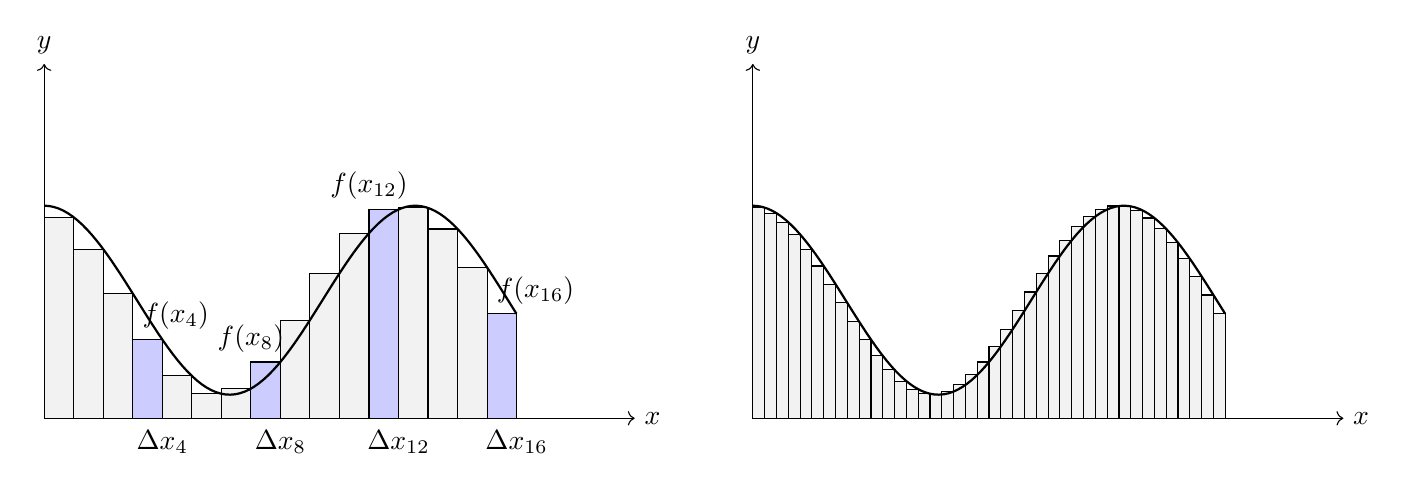
\begin{tikzpicture}[scale=1.5]
% Define the function
\def\f(#1){0.8*cos(deg(2*#1)) + 1}

% Draw the x-axis
\draw[->] (0,0) -- (5,0) node[right] {$x$};
% Draw the y-axis
\draw[->] (0,0) -- (0,3) node[above] {$y$};


% Draw the rectangles for the Riemann sum
\draw[fill=gray!10] (0, 0) rectangle (.25, {\f(.25)});
\draw[fill=gray!10] (.25, 0) rectangle (.5, {\f(.5)});
\draw[fill=gray!10] (.5, 0) rectangle (.75, {\f(.75)});
\draw[fill=blue!20] (0.75, 0) rectangle (1, {\f(1)});
\draw[fill=gray!10] (1, 0) rectangle (1.25, {\f(1.25)});
\draw[fill=gray!10] (1.25, 0) rectangle (1.5, {\f(1.5)});
\draw[fill=gray!10] (1.5, 0) rectangle (1.75, {\f(1.75)});
\draw[fill=blue!20] (1.75, 0) rectangle (2, {\f(2)});
\draw[fill=gray!10] (2, 0) rectangle (2.25, {\f(2.25)});
\draw[fill=gray!10] (2.25, 0) rectangle (2.5, {\f(2.5)});
\draw[fill=gray!10] (2.5, 0) rectangle (2.75, {\f(2.75)});
\draw[fill=blue!20] (2.75, 0) rectangle (3, {\f(3)});
\draw[fill=gray!10] (3, 0) rectangle (3.25, {\f(3.25)});
\draw[fill=gray!10] (3.25, 0) rectangle (3.5, {\f(3.5)});
\draw[fill=gray!10] (3.5, 0) rectangle (3.75, {\f(3.75)});
\draw[fill=blue!20] (3.75, 0) rectangle (4, {\f(4)});

% Draw the curve
\draw[thick, domain=0:4, samples=100] plot (\x, {\f(\x)});

% Draw the labels for f(xi)
\draw (0.75, {\f(1)}) node[above right] {$f(x_{4})$};
\draw (1.75, {\f(2)}) node[above] {$f(x_{8})$};
\draw (2.75, {\f(3)}) node[above] {$f(x_{12})$};
\draw (3.75, {\f(4)}) node[above right] {$f(x_{16})$};

% Draw the arrows for delta x

\draw (1, -0.2) node {$\Delta x_{4}$};
\draw (2, -0.2) node {$\Delta x_{8}$};
\draw (3, -0.2) node {$\Delta x_{12}$};
\draw (4, -0.2) node {$\Delta x_{16}$};

	\begin{scope}[xshift=6cm]
	% Define the function
	\def\f(#1){0.8*cos(deg(2*#1)) + 1}
	
	% Draw the x-axis
	\draw[->] (0,0) -- (5,0) node[right] {$x$};
	% Draw the y-axis
	\draw[->] (0,0) -- (0,3) node[above] {$y$};
	
	
	  % Draw the rectangles for the Riemann sum
	\foreach \xi in {0.1, 0.2, ..., 4} {
		\draw[fill=gray!10] (\xi-0.1, 0) rectangle (\xi, {\f(\xi)});
	}
	
	
	% Draw the curve
	\draw[thick, domain=0:4, samples=100] plot (\x, {\f(\x)});
	
	\end{scope}
\end{tikzpicture}
  \caption{A visualization of the Riemann Sums. The partition width is denoted by $\Delta x_i$ and the height of the partitions is $f(x_i)$.}
  \label{fig:Riemann Sum visualization}
\end{figure}

\begin{defn}[Riemann Sum\label{defn:Riemann Sum]{1}
Let $f$ be defined on the closed interval $[a,b]$, and let $\Delta$ be a partition of $[a,b]$ given by $a=x_0 < x_1 < \cdots < x_{n-1} < x_n = b$, where $\Delta x_i$ is the width of the $i$th sub-interval. If $c_i \in [x_{i-1},x_i]$, then the sum $\sum_{i=1}^{n}f(c_i)\Delta x_i$ is called a Riemann sum of $f$ for the partition $\Delta$.
\end{defn}

The largest width among the subintervals within a partition $\Delta$ is known as the partition's norm, represented by $||\Delta||$. If all subintervals have equal width, the partition is called regular, and its norm is denoted by $||\Delta|| = \Delta x = \frac{b-a}{n}$. The integral can be defined in the limit as this partition's norm approaches zero $||\Delta|| \to 0$. Therefore, there exists some $L\in\mathbf{R}$ such that for each $\epsilon > 0$, there exists a $\delta > 0$ so that for all partitions with $||\Delta|| < \delta$, we have

\begin{align}
\lim_{||\Delta|| \to 0}\sum_{i=1}^{n}f(c_i)\Delta x_i = L \implies \bigg|L-\sum_{i=1}^{n}f(c_i)\Delta x_i\bigg| < \epsilon
\end{align}

This then give the definition of the definite integral.

\begin{defn}[The Definite Integral\label{defn:The Definite Integral}]{1}
IF $f$ is defined on the closed interval $I=[a,b]$ and the limit of the Riemann sums over partitions $\Delta$ exists, then $f$ is said to be integrable on $I$ and the limit is denoted by the definite integral of $f$ from $a$ to $b$. 
\begin{align}
\lim_{||\Delta|| \to 0}\sum_{i=1}^{n}f(c_i)\Delta x_i = \int_a^b f(x)dx
\end{align}
\end{defn}

%\begin{theo}[The Fundamental Theorem Of Calculus]{1}
%Suppose that $f(x)$ is continuous on the interval [a,b]. If $F(x)$ is any antiderivative of $f(x)$, then $\int_a^b f(x) dx = F(b)-F(a)$. Given $F(x) = \int_a^b f(x) dx$, then $\frac{d}{dx}F(x) = f(x)$.
%\end{theo}


\newpage
\chapter{General Physics}
\thispagestyle{fancy}

Physics is the scientific study of the fundamental principles that govern the behavior of matter, energy, space, and time. It seeks to understand the natural world by formulating and testing mathematical models and theories based on observations and experimental evidence. Physics is a broad and diverse field that encompasses various sub-disciplines, including classical mechanics, electromagnetism, thermodynamics, quantum mechanics, and relativity, among others. Key areas of study in physics include:

\begin{itemize}
	\item \keyword{Classical Mechanics}: This branch deals with the motion of macroscopic objects and is based on Newton's laws of motion and the concept of conservation of energy and momentum.

	\item \keyword{Electromagnetism}: This field explores the behavior of electric and magnetic fields and their interactions with charged particles, leading to the understanding of electricity, magnetism, and electromagnetic waves.

	\item \keyword{Thermodynamics}: It examines the relationships between heat, work, and energy, providing insights into the behavior of gases, liquids, and solids and the principles of heat engines and refrigeration.

	\item \keyword{Quantum Mechanics}: This revolutionary theory describes the behavior of particles at the atomic and subatomic levels, often challenging our classical intuitions and introducing concepts like wave-particle duality and quantum entanglement.

	\item \keyword{Relativity}: Special and General Relativity, proposed by Albert Einstein, deal with the nature of space, time, and gravity, especially at high speeds and in the presence of massive objects.

	\item \keyword{Nuclear Physics}: It focuses on the study of atomic nuclei, nuclear reactions, and nuclear forces, leading to applications in energy production and understanding the universe's early moments.

	\item \keyword{Particle Physics}: This field investigates the fundamental particles of the universe and their interactions, exploring the subatomic realm with particle accelerators and detectors.

	\item \keyword{Astrophysics}: The study of celestial objects and phenomena, such as stars, galaxies, black holes, and cosmic rays, to understand the structure and evolution of the universe.

Condensed Matter Physics: It examines the properties of solid and liquid matter and studies phenomena like superconductivity, magnetism, and phase transitions.
\end{itemize}

Physics has been crucial in advancing technology and shaping our understanding of the universe, from everyday applications like electronics and telecommunications to groundbreaking discoveries about the fundamental nature of reality. It plays a central role in modern science and continues to be a driving force for innovation and progress in various fields. Physics stands as the foundational and all-encompassing science, profoundly shaping the advancement of all scientific disciplines.

\begin{interestnote}
	A poet once said, “The whole universe is in a glass of wine.” We will probably never know in what sense he meant that, for poets do not write to be understood. But it is true that if we look at a glass of wine closely enough we see the entire universe. There are the things of physics: the twisting liquid which evaporates depending on the wind and weather, the reflections in the glass, and our imagination adds the atoms. The glass is a distillation of the earth’s rocks, and in its composition we see the secrets of the universe’s age, and the evolution of stars. What strange array of chemicals are in the wine? How did they come to be? There are the ferments, the enzymes, the substrates, and the products. There in wine is found the great generalization: all life is fermentation. Nobody can discover the chemistry of wine without discovering, as did Louis Pasteur, the cause of much disease. How vivid is the claret, pressing its existence into the consciousness that watches it! If our small minds, for some convenience, divide this glass of wine, this universe, into parts—physics, biology, geology, astronomy, psychology, and so on—remember that nature does not know it! So let us put it all back together, not forgetting ultimately what it is for. Let it give us one more final pleasure: drink it and forget it all! \cite{bib:feynman lectures}
\end{interestnote}


\section{Measurement}

\keyword{Measurement} is one of the most important tools for studying physics as it relates to a physical reality. A measurement always has some sort of error associated with it and is always relative to \textit{something}.

\begin{quotation}
	``Wherefore relative quantities are not the quantities themselves, whose names they bear, but those sensible measures of them (either accurate or inaccurate), which are commonly used instead of the measured quantities themselves. And if the meaning of words is to be determined [definiendae] by their use, then by the names time, space, place, and motion, their measures [mensurae sensibilies] are properly to be understood; and the expression will be unusual, and purely mathematical, if the measured quantities themselves are meant. On this account, those violate the accuracy of language, which ought to be kept precise, who interpret these words for the measured quantities. Nor do those less defile the purity of mathematical and philosophical truths, who confound real quantities with their relations and sensible measures [vulgaribus mensuris].'' \cite{bib:Newtons Scholium}
\end{quotation}


\section{Chemistry}

\keyword{Inorganic chemistry} is the branch of chemistry that deals with the study of inorganic compounds, which are substances not primarily based on carbon-hydrogen (C-H) bonds. It explores the properties, structures, and behaviors of minerals, metals, gases, and other inorganic substances, playing a crucial role in understanding the fundamental elements and their interactions. The theory of chemistry and chemical reactions, was summarized to a large extent in the periodic chart of \keyword{Mendeleev}, also known as the \keyword{periodic table of elements}. All of these rules were eventually explained by quantum mechanics and thus theoretical chemistry is actually just physics. \keyword{Organic chemistry} is the chemistry of substances which are associated with living things. These are typically complex. This field is closely related to biology.

\keyword{Statistical mechanics} was a branch of physics developed alongside chemistry and has played an extremely important role in history. In any chemical situation, there are a large number of atoms all interacting. If all of these atoms could be analyzed at each collision and kept track of, the phenomenon of chemical reactions could be predicted. Statistical mechanics is the science of heat or thermodynamics which accomplishes this to some degree.

\section{Biology}

\keyword{Biology} is the scientific study of living organisms and their interactions with the environment. It encompasses a wide range of topics, from the molecular and cellular levels to the study of ecosystems and biodiversity. Biology seeks to understand the processes of life, including growth, reproduction, adaptation, and evolution, providing insights into the diversity and complexity of living systems. Biology is composed of many physical phenomenon and systems which can be studies and understood by physics. There are often very intriguing connections between physics and biology. The \keyword{conservation of energy} was in large part inspired by biology when Julius von Mayer demonstrated a connection with the amount of heat taken in and given out by a living creature. Another example is that of nerves which function as very find tubes with positive ions on the outside and negative ions on the inside - much like a capacitor that can be discharged to send signals.

\keyword{Proteins} are large, complex molecules composed of amino acids, essential for various biological functions. They play crucial roles in the structure, function, and regulation of cells and tissues, serving as enzymes, receptors, transporters, and antibodies. \keyword{Enzymes}, a specialized type of protein, act as biological catalysts, speeding up chemical reactions within cells. They are highly specific and crucial for metabolic processes, allowing cells to carry out essential tasks such as digestion, energy production, and DNA replication. A significant achievement since the 1960s has been the precise determination of the atomic arrangement in certain proteins, comprising approximately fifty-six or sixty amino acids in sequence. These studies have located over a thousand atoms, including hydrogen atoms, forming intricate patterns in some proteins, such as \keyword{hemoglobin}. Despite this progress, the mystery remains as to why these patterns function as they do.

\keyword{DNA}, short for deoxyribonucleic acid, is a molecule that carries genetic information in all living organisms. It consists of a double helix structure made up of nucleotide units, each containing a sugar, phosphate group, and a nitrogenous base. DNA serves as the blueprint for the development, functioning, and inheritance of living beings, encoding the instructions required for the synthesis of proteins and controlling various cellular processes. The study of DNA's structure led to the remarkable discovery that it consists of a pair of twisted chains, with specific cross-links between them. These cross-links, represented by adenine, thymine, cytosine, and guanine, fit together in pairs. The pairs form strong bonds and only certain pairs will create these bonds. Therefore, when DNA is split, there is only one way to reproduce the other half in cell reproduction, ensuring the accurate replication of DNA during cell division and passing on specific instructions for protein synthesis to offspring.

No subject or field is making more progress on so many fronts at the present moment, than biology, and if we were to name the most powerful assumption of all, which leads one on and on in an attempt to understand life, it is that all things are made of atoms (see \ref{section:The Atomic Hypothesis}), and that everything that living things do can be understood in terms of the jigglings and wigglings of atoms.

\section{Astronomy}

\keyword{Astronomy} is the scientific study of celestial objects, phenomena, and the universe as a whole. It encompasses the observation, analysis, and understanding of stars, planets, galaxies, and other cosmic structures, as well as the exploration of space and the fundamental principles governing the cosmos. Astronomy plays a crucial role in unraveling the mysteries of the universe, from studying the origins of galaxies to investigating the properties of distant exoplanets and the evolution of the cosmos over billions of years. Astronomy is older than physics and bridged the way for the beginning of physics through observations of the simplistic motion of starts and planets. 

The most remarkable discovery in all of astronomy is that the stars are made of atoms of the same kind as those on the earth. With a \keyword{spectroscope}, we can analyze the frequencies of light waves and can therefore see the presence of atoms that are in different stars. Some chemicals were even discovered in stars before being discovered on earth.

One of the most impressive discoveries was the origin of energy in stars. The nuclear `burning' of hydrogen supplies energy to stars. The stellar properties inside stars make them prime conditions for many nuclear reactions to occur and new elements to be created. The isotopic proportions in our own composition reveal the stellar origins of the elements, suggesting that we were "cooked" in stars and expelled through novae and supernovae explosions. Astronomy, closely linked to physics, offers valuable insights into these processes.

\section{Geology}

\keyword{Geology}, also called \keyword{earth sciences}, is the scientific study of the Earth's structure, composition, and processes that have shaped its history. It investigates the formation of rocks, minerals, and geological features, such as mountains, volcanoes, and earthquakes, as well as the evolution of landscapes and the interactions between the Earth's materials and natural forces. Geology plays a crucial role in understanding Earth's past, present, and future, and it contributes to various fields, including resource exploration, environmental management, and hazard assessment. The question basic to geology is, what makes the earth the way it is?

Meteorology is the scientific study of the Earth's atmosphere and weather phenomena. It closely relates to physics because it involves the application of fundamental physical principles, such as thermodynamics, fluid dynamics, and radiation, to understand and predict atmospheric processes. By analyzing the behavior of air masses, temperature, humidity, pressure, and wind patterns, meteorologists use physics-based models and observations to forecast weather conditions and study atmospheric phenomena like hurricanes, tornadoes, and climate change. The interaction between meteorology and physics plays a crucial role in advancing our understanding of the Earth's atmosphere and its impact on weather patterns and climate dynamics.

While we have considerable knowledge about earthquake waves and the Earth's density distribution, physicists face challenges understanding matter's properties at the immense pressures within the Earth's core. Unlike conditions in stars, the complex mathematics involved in these extreme circumstances remains a hurdle to tackle. Additionally, determining the density and behavior of rocks at high pressure requires experimental investigations, as our theoretical understanding is limited.




\section{Energy}

The \keyword{conservation of energy} is believed to be a fundamental law governing all known natural phenomena that are known to date. It is an exact and unbroken principle, stating that a quantity known as \keyword{energy} remains constant amidst the various changes occurring in nature. This abstract idea is based on mathematical principles, representing a numerical quantity that remains unchanged throughout different events. It is not a description of a concrete mechanism but rather a remarkable fact: the calculated energy value remains the same after observing nature's transformations. Energy has a large number of different forms, and there is a formula for each one. These are: gravitational energy, kinetic energy, heat energy, elastic energy, electrical energy, chemical energy, radiant energy, nuclear energy, mass energy. If we total up the formulas for each of these contributions in a system, it will not change except for energy going in and out of the system.

In quantum mechanics it turns out that the conservation of energy is very closely related to another important property of the world, \textit{things do not depend on the absolute time}.

\subsection{Gravitational Potential Energy}

The general name of energy which has to do with location relative to something else is called \keyword{potential energy}. In the case of objects relative to earth (or other bodies effected by gravitational energy), it is called \keyword{gravitational potential energy}.
	
\begin{defn}[Gravitational Potential Energy \label{Gravitational Potential Energy Definition}]
	Gravitational potential energy $E$ is a form of potential energy associated with the position of an object in a gravitational field. It represents the energy stored in an object due to its height $h$ above a reference point. The higher an object is positioned above the reference point, the greater its gravitational potential energy.
	\begin{align}
		E = mgh,
	\end{align}
	where $m$ is the mass of the object and $g$ is the acceleration due to gravity.
\end{defn}

For static structures and systems, one can apply an imaginary motion to the system (even if it is not really moving or even movable) in order to apply the principal of conservation of energy. This approach is called the \keyword{principle of virtual work}.

\subsection{Kinetic Energy}

The principal of \keyword{motion} gives rise to another type of energy referred to as \keyword{kinetic energy}.

\begin{defn}[Kinetic Energy \label{Kinetic Energy}]
	Kinetic energy $E$ is a fundamental concept in physics that refers to the energy possessed by an object due to its motion. It is the energy associated with the object's velocity and is dependent on both its mass $m$ and the square of the magnitude of its velocity $v$. 
	\begin{align}
		E = \frac{1}{2}mv^2
	\end{align}
\end{defn} 

when associated with relativity, there is a modification to this concept of kinetic energy. An object has energy from simply existing which is referred to as a mass energy which is combined with this kinetic energy of motion.


















\newpage
\chapter{Classical Mechanics}
\thispagestyle{fancy}

\keyword{Classical mechanics} is a branch of physics that describes the motion of objects and systems under the influence of forces. It forms the foundation of mechanics before the advent of quantum mechanics and relativistic physics. Classical mechanics is based on Newton's laws of motion and the concept of conservation of energy and momentum. Key principles and concepts of classical mechanics include:

\begin{itemize}
	\item \keyword{Newton's Laws of Motion}: Sir Isaac Newton formulated three fundamental laws that govern the motion of objects. The first law (Law of Inertia) states that an object at rest remains at rest, and an object in motion continues to move at a constant velocity unless acted upon by an external force. The second law describes how the acceleration of an object is directly proportional to the net force applied and inversely proportional to its mass. The third law states that for every action, there is an equal and opposite reaction.
	
	\item \keyword{Conservation of Energy}: The principle of energy conservation states that the total energy of an isolated system remains constant over time. Energy can transform from one form to another (e.g., kinetic energy to potential energy), but the total amount of energy remains unchanged.
	
	\item \keyword{Conservation of Momentum}: The principle of momentum conservation states that the total momentum of an isolated system remains constant, provided no external forces act on it. Momentum is the product of an object's mass and velocity.
	
	\item \keyword{Gravitation}: Classical mechanics includes the study of gravitational forces between objects, described by Newton's law of universal gravitation. This law explains how objects attract each other with a force proportional to their masses and inversely proportional to the square of the distance between them.
	
	\item \keyword{Harmonic Motion}: The study of harmonic motion involves oscillations and vibrations of systems, such as a pendulum or a mass-spring system. These motions follow simple harmonic motion equations and exhibit periodic behavior.
\end{itemize}

Classical mechanics provides accurate and practical predictions for a wide range of everyday scenarios and macroscopic systems. While it is highly effective in describing the behavior of objects at non-relativistic speeds, it becomes less accurate when dealing with extremely high speeds or microscopic particles, where quantum mechanics and relativistic physics are more appropriate. Nonetheless, classical mechanics remains a crucial and fundamental branch of physics, forming the basis for understanding the motion of everyday objects and engineering applications.


\section{Gravity}

The law of gravitation is that every object in the universe attracts every other object with a force which for any two bodies is proportional to the mass of each and varies inversely as the square of the distance between them. This is typically mathematically represented as

\begin{align}
F = \frac{Gm_1m_2}{r^2}
\end{align}

While we can describe how gravity works mathematically, its underlying mechanism remains somewhat unknown. The absence of a known mechanism drives scientific inquiry, leading to further discoveries. No mechanism has been devised to "explain" gravity without simultaneously predicting the existence of some other phenomenon. To a great precision, this force is exactly proportional to mass, and therefore fundamentally related to \keyword{inertia}.

\begin{questions}
	\item Is this law a constant through time - perhaps the constant changes?
	\item Does this law somehow relate to the force of electrical attraction since they are both proportional to the inverse of the distance squared?
\end{questions}

\begin{interestnote}
	The relative strengths of electrical and gravitational interactions between two electrons is
 	\begin{align}
  		\frac{\text{Gravitation Attraction}}{\text{Electrical Repulsion}} = \frac{1}{4.17\times 10^{42}}.
  	\end{align}
   	If we compare the time it takes for light to go across a proton ($10^{-24}$ seconds) to the age of the universe, which is approximately $2\times 10^{10}$ years, the result is $10^{-42}$. They both have a similar number of zeros, leading to a potential idea that the gravitational constant may be linked to the age of the universe.
\end{interestnote}

\subsection{Keplar's Laws}

Johannes Kepler was a German mathematician, astronomer, and astrologer who made significant contributions to our understanding of the solar system and planetary motion during the late 16th and early 17th centuries. Kepler is best known for formulating three fundamental laws of planetary motion, which laid the groundwork for modern astronomy. These laws were based on careful observations made by Tycho Brahe. \keyword{Kepler's laws} are
\begin{enumerate}
	\item Each planet moves around the sun in an ellipse, with the sun at one focus.
 	\item The radius vector from the sun to the planet sweeps out equal areas in equal intervals of time.
  	\item The squares of the periods of any two planets are proportional to the cubes of the semi-major axes of their respective orbits: $T\propto a^{3/2}$.
\end{enumerate}

Galileo was studying these laws when he discovered the principal of \keyword{inertia}-\textit{if something is moving, with nothing touching it and completely undisturbed, it will go on forever, coasting at a uniform speed in a straight line.}

\begin{questions}
	\item What is the cause of inertia?
 	\item Does an objects inertia lower over time?
\end{questions}

Newton further extended this by introducing the idea of a \keyword{force}. If a body is to change speed or direction, a force must be applied to it in the direction of the change. This gives the understanding that there must be a force acting on planets in order to keep them in rotation around the sun - rather than just flying off into space.








\section{Motion}

keyword{Motion} is the change in the position of an object relative to a reference point over time. It involves the displacement of an object from one location to another in a continuous manner. Motion can occur in various forms, such as \keyword{linear motion} (movement along a straight line), \keyword{circular motion} (movement in a circular path), \keyword{rotational motion} (movement around a fixed axis), or \keyword{oscillatory motion} (back-and-forth movement around a central position). 

\keyword{Velocity} is a vector quantity that describes the rate of change of an object's position with respect to time. It specifies both the speed and the direction of an object's motion. Velocity $\vec{v}$ is calculated by dividing the displacement (change in position) $\Delta x$ of the object by the time taken to cover that displacement $\Delta t$. Velocity is expressed in units of distance per unit of time, such as meters per second (m/s) or kilometers per hour (km/h). If the velocity is constant over time, it is referred to as constant velocity, and if the velocity is changing, it is referred to as variable velocity. When the direction of an object's motion remains constant, the velocity is considered to be uniform; otherwise, it is non-uniform. Velocity plays a crucial role in describing and analyzing the motion of objects in physics and other scientific disciplines.
\begin{align}
\vec{v}(t)=\lim_{\Delta t \to 0}\frac{\Delta \vec{x}(t)}{\Delta t} = \frac{d\vec{x}(t)}{dt} \implies \vec{x}(t) = \int \vec{v}(t) dt
\end{align}

\keyword{Acceleration} is a vector quantity that describes the rate of change of an object's velocity with respect to time. It indicates how quickly an object's velocity is changing or how much the object is speeding up or slowing down. Acceleration is defined as the change in velocity divided by the change in time. Acceleration, like velocity, is a vector quantity, meaning it has both magnitude and direction. If an object is moving in a straight line, acceleration is in the same direction as the net force acting on the object. If the object is moving in a curved path, the acceleration is directed towards the center of the curvature. The units of acceleration are typically expressed as distance per unit time squared, such as meters per second squared (m/s$^2$) or centimeters per second squared (cm/s$^2$).
\begin{align}
\vec{a}(t)=\lim_{\Delta t \to 0}\frac{\Delta \vec{v}(t)}{\Delta t} = \frac{d\vec{v}(t)}{dt} = \frac{d^2\vec{x}(t)}{dt^2} \implies \vec{v}(t) = \int \vec{a}(t) dt
\end{align}

\keyword{Jerk} is a vector quantity that represents the rate of change of acceleration with respect to time. In other words, jerk measures how quickly an object's acceleration is changing or how rapidly the object's rate of change in velocity is varying. Jerk is a vector quantity, just like acceleration and velocity, meaning it has both magnitude and direction. However, jerk is less commonly used in everyday physics problems compared to acceleration, which is more frequently encountered. In most cases, acceleration is sufficient to describe the motion of objects, and jerk is not a significant factor in standard physics analysis. Nonetheless, jerk becomes relevant in certain specialized fields, such as robotics, aerospace engineering, and studies involving rapid changes in motion or acceleration profiles.
\begin{align}
\vec{j}(t)=\lim_{\Delta t \to 0}\frac{\Delta \vec{a}(t)}{\Delta t} = \frac{d\vec{a}(t)}{dt} = \frac{d^2\vec{v}(t)}{dt^2} = \frac{d^3\vec{x}(t)}{dt^3} \implies \vec{a}(t) = \int \vec{j}(t) dt
\end{align}


\subsection{Newton's Laws}

\keyword{Momentum} $\vec{p}$ is a vector quantity that measures the quantity of motion possessed by an object. It is the product of an object's mass and its velocity and is a fundamental concept in classical mechanics. In this context, \keyword{Mass} is a quantitative measure of \keyword{inertia} (resistance to being accelerated). Since momentum is a vector, it has both magnitude and direction. The direction of the momentum vector is the same as the direction of the velocity vector. The SI unit of momentum is kilogram-meter per second (kg·m/s).

\begin{align}
	\vec{p} = m\vec{v}
\end{align}

Following Galileo's discovery of the principal of \keyword{inertia}, Newton set out to describe the rules for finding out how an object changes its \keyword{motion} when effected by something.

\begin{fancybox}[Newton's Laws Of Motion]{1}
	\begin{enumerate}
		\item \keyword{The Law of Inertia}: An object at rest will remain at rest, and an object in motion will continue to move with a constant velocity in a straight line unless acted upon by an external force./footnote{This is simply a restating of Galileo's described principal of inertia.}
		\item The time-rate-of-change of a quantity called momentum is proportional to the force.
		\begin{align}
			\vec{F}=\frac{d\vec{p}}{dt} = m\frac{d\vec{v}}{dt} = m\frac{d^2\vec{x}}{dt^2} = m\vec{a}
		\end{align}
		The two forms of this law $\vec{F}=m\vec{a}$ and $\vec{F}=\frac{d\vec{p}}{dt}$ are \textit{not} equivalent in with respect to relativity.
		\item For every action, there is an equal and opposite reaction.
	\end{enumerate}
\end{fancybox}

Since relativity and quantum mechanics were formulated, it has been known that these laws are not universally valid and only a highly accurate approximation for classical physics scenarios.


\subsection{Inertial Frames}

An \keyword{inertial reference frame}, also known as an \keyword{inertial frame} of reference or simply an inertial frame, is a specific coordinate system or frame of reference in which Newton's first law of motion holds true. In an inertial reference frame, an object at rest remains at rest, and an object in motion with constant velocity continues to move in a straight line with the same velocity unless acted upon by an external force. Alternatively, an inertial reference frame is a coordinate system that is not accelerating and has no net force acting on it. In such a frame, objects move freely and uniformly in accordance with Newton's laws of motion without any additional forces or accelerations introduced by the frame itself. Newton's second law, given no net force on an object ($\vec{F}=0$) gives an acceleration of zero ($a=0$). This suggests that Newton's second law includes the first. However, this is only the case in an \keyword{inertial frame}. The laws of motion only hold in inertial frames and an \keyword{inertial frame} is defined as one where \keyword{the law of inertia} holds.



\newpage
\chapter{Electronics}
\thispagestyle{fancy}

\keyword{Electronics} is a multidisciplinary field that revolves around the study and manipulation of electrons and their behavior in different materials and devices. This field has revolutionized the way we communicate, compute, and interact with the world, giving rise to an unprecedented era of technological advancements. Electronics encompasses a vast range of topics, from the fundamental principles of semiconductor physics to the design and development of intricate integrated circuits, enabling the creation of devices that have become an integral part of our daily lives. Key Concepts in Electronics include the following:

\begin{itemize}
	\item \keyword{Semiconductors}: Semiconductors are materials that have properties between conductors (like metals) and insulators. The behavior of electrons in semiconductors is crucial to the operation of electronic devices. By manipulating the conductivity of semiconductors, devices like transistors and diodes can be created.

    \item \keyword{Transistors}: Transistors are fundamental building blocks of modern electronics. They act as switches or amplifiers, controlling the flow of electrical current by varying a small input signal. Transistors are the core components of integrated circuits (ICs), which power computers, smartphones, and a myriad of other devices.

    \item \keyword{Integrated Circuits}: Integrated circuits (ICs) are miniaturized collections of electronic components, such as transistors, resistors, and capacitors, fabricated on a single semiconductor wafer. They range from simple logic gates to complex microprocessors, enabling the creation of highly compact and powerful devices.

    \item \keyword{Digital} vs. \keyword{Analog}: Electronics deals with both digital and analog signals. Digital electronics represent information using discrete values (0s and 1s), forming the basis of computers and digital communication systems. Analog electronics, on the other hand, work with continuous signals and are essential for tasks like audio processing.

    \item \keyword{Circuit Design}: Circuit design involves creating schematics and layouts for electronic circuits. Design considerations include selecting components, optimizing power consumption, managing heat dissipation, and ensuring reliable operation.

    \item \keyword{Power Electronics}: Power electronics focuses on the conversion and control of electrical power. This field is vital for technologies such as power supplies, motor drives, renewable energy systems, and electric vehicles.

    \item \keyword{Signal Processing}: Signal processing involves manipulating signals to extract, enhance, or encode information. It's used in applications like image and audio processing, telecommunications, and control systems.

    \item \keyword{Microcontrollers} and \keyword{Microprocessors}: Microcontrollers are small computers on a single chip, often used to control specific tasks in devices like household appliances and automotive systems. Microprocessors are the brains of computers and smartphones, executing complex instructions and tasks.

    \item \keyword{Printed Circuit Boards} (PCBs): PCBs provide a platform for connecting and mounting electronic components. They are found in virtually all electronic devices and play a crucial role in determining a device's functionality and reliability.
\end{itemize}


\section{Basics}

\begin{defn}[Conductors]{defn:conductor}
An electrical \keyword{conductor} is a substance where the electrons are mobile.
\end{defn}

Copper and Aluminum are excellent conductors and other metals such as iron and steel range from fair to good conductors.

\begin{interestnote}
One of the best conductors at room temperature is pure elemental silver. 
\end{interestnote}

\begin{defn}[Insulators]{defn:insulator}
An electrical \keyword{insulator} is a substance that prevents current from flowing.
\end{defn}

Most gases are good electrical insulators. Glass, dry wood, paper, and plastics are examples. 

\begin{interestnote}
Pure water is a good insulator but the slightest impurity can cause it to conduct current.
\end{interestnote}

\begin{defn}[Resistors]{defn:resistors}
\keyword{Resistors} are electrical components made to allow for the control of current flow. This is typically done by changing the size, shape, or adding impurities to a substance. Electrical resistance is measured in units called \keyword{ohms}.
\end{defn}

Resistance is often references as per a unit length (ohms per foot, etc). resistance also converts electrical energy into heat, and therefore low resistance is generally desired in electrical systems. 

\begin{defn}[Semiconductor]{defn:semiconductor}
A \keyword{semiconductor} is a substance that has a conductivity between an insulator and that of most metal conductors.
\end{defn}

Semiconductors are typically made from adding impurities or changing the temperature conditions. Silicon is a notable semiconductor that is common in electronic circuits. Indium or antimony are often used to dope silicon, selenium or gallium to create semiconductors. A \keyword{hole} is a shortage of an electron, and the movement of holes is often used as reference rather than the movement of electrons. When the charge carriers are electrons, a semiconductor is N-type (because the electrons are negatively charged). When the majority of the charge carriers are holes, a semiconductor is called P-type (since the absence of the negative electron creates a positive charge).

\begin{defn}[Current]{defn:current}
\keyword{Current} can be defined as the movement of charge carriers in a substance. Current is measured in terms of the number of charge carriers passing a single point in a second in units of \keyword{coulombs}\footnote{A coulomb is a measure of charge and is equivalent to approximately $6.24 \times 10^{18}$ charge carriers (electrons or holes).} per second. Another name for this unit is an \keyword{Ampere}.
\end{defn}









\newpage
\chapter{Acoustics}
\thispagestyle{fancy}

\keyword{Acoustics} is the scientific study of sound and its transmission, production, and effects. It is a branch of physics and engineering that explores the properties of sound waves, their interactions with various mediums, and their impact on our environment and human perception. Acoustics plays a crucial role in our everyday lives, from the design of concert halls and the development of audio technology to the understanding of natural phenomena like earthquakes and the behavior of underwater sound.

At its core, \keyword{acoustics} seeks to unravel the mysteries of sound, a complex and omnipresent phenomenon that shapes our auditory experiences and contributes to our understanding of the world. Acoustics is not just the study of auditory sound though. At its core, acoustics is the study of vibrations propogating through matter, which in some ways is the study of everything and plays a critical role in the universe and matter interactions.

\section{Units}

The fundamental unit of sound change is called the \keyword{decibel} (dB). Perceived levels of sound change according to a logarithmic relation of the actual power levels. Decibels are calculated relative to a ratio of change from power $P_1$ watts to a power $P_2$ watts. The change in decibels is then
\begin{align}
dB = 10 \log_{10}\left(\frac{P_2}{P_1}\right)
\end{align}














\section{Underwater Acoustics}

Large bodies of water, such as the large ones covering Earth's surface do not allow for the propogation of radio and radar waves. Water, especially salt water is highly dissipative because it exhibits strong conductivity. This conductivity atteniates electromagnetic waves extremely rapidly, which limits their range and usefulness. Therefore, acoustic waves are the more practical way of carrying information underwater \cite{bib:An Introduction To Underwater Acoustics}. Acoustic waves have different transmission characteristics in water than they do in air. Some advantages in water are that they have a propogation speed or four to five times higher than in air, they reach higher levels, and they undergo less attentiation and therefore can propogate over larger distances\footnote{Sound propogation in the ocean can be observed at rangest of thousands of kilometers\cite{bib:An Introduction To Underwater Acoustics}.}. Some typical constraints include higher ambient noise levels, and more echos. Many species utilize use of sound waves in oceans such as whales and cataceans. 


\newpage
\chapter{Optics}
\thispagestyle{fancy}

Optics is the study of light motions including reflection, refraction, diffraction, and interference. 


\newpage
\chapter{Statistical Mechanics \& Thermodynamics}
\thispagestyle{fancy}

\keyword{Statistical mechanics} is a branch of physics that aims to explain the macroscopic properties of a system (such as temperature, pressure, and entropy) by understanding the behavior and interactions of its microscopic constituents at the atomic or molecular level. It bridges the gap between the microscopic world of particles and the macroscopic world we observe in everyday life. Key concepts and principles of statistical mechanics include:

\begin{itemize} 
	\item \keyword{Microstates} and \keyword{Macrostates}: In statistical mechanics, a system's microstate refers to the specific arrangement and energy distribution of its individual particles. A macrostate, on the other hand, represents the observable properties of the system, such as its temperature, pressure, and volume. The goal of statistical mechanics is to determine the probabilities of different microstates leading to a given macrostate.
	
	\item \keyword{Ensembles}: Statistical mechanics uses ensembles, which are collections of similar systems, to study statistical properties. Common ensembles include the microcanonical ensemble (isolated system with constant energy), canonical ensemble (system in thermal contact with a heat reservoir), and grand canonical ensemble (system with exchange of energy and particles with a heat reservoir).
	
	\item \keyword{Boltzmann Distribution}: The Boltzmann distribution relates the probabilities of different energy states to their corresponding energies and the system's temperature. It allows us to predict how particles are distributed among different energy levels in a system.
	
	\item \keyword{Entropy} and Entropy Maximization: Entropy is a fundamental concept in statistical mechanics, representing the measure of a system's disorder or randomness. The second law of thermodynamics states that isolated systems tend to evolve toward states of higher entropy. Statistical mechanics provides a statistical interpretation of entropy and explains the tendency of systems to maximize their entropy over time.
	
	\item \keyword{Statistical Thermodynamics}: Statistical mechanics connects with thermodynamics, relating the macroscopic thermodynamic properties (e.g., internal energy, temperature, and heat capacity) to the statistical properties of microscopic constituents. This connection allows us to derive thermodynamic quantities from the statistical behavior of particles.
\end{itemize}

Statistical mechanics has wide-ranging applications in various scientific disciplines, including physics, chemistry, biology, and materials science. It is essential for understanding phase transitions, chemical reactions, and the behavior of matter under different conditions. Additionally, statistical mechanics forms the basis for exploring complex systems, such as gases, liquids, and solids, and plays a crucial role in the development of many modern technologies.

\newpage
\chapter{Astrophysics}
\thispagestyle{fancy}


\newpage
\chapter{Electromagnetism}
\thispagestyle{fancy}


\newpage
\chapter{Quantum Mechanics}
\thispagestyle{fancy}

\keyword{Quantum mechanics} is a fundamental branch of physics that describes the behavior of matter and energy at the smallest scales, such as subatomic particles and photons. It provides a unique and revolutionary framework for understanding the peculiar and counterintuitive behavior of particles at the quantum level. Key concepts and principles of quantum mechanics include:

\begin{itemize}
	\item \keyword{Wave-Particle Duality}: One of the central tenets of quantum mechanics is the wave-particle duality. It states that particles, such as electrons and photons, exhibit both particle-like and wave-like characteristics. They can be described by wave functions, which represent probabilities of finding a particle at different locations.

	\item \keyword{Quantization of Energy}: Quantum mechanics introduced the concept of quantized energy levels, where energy levels of particles are restricted to discrete values rather than continuous values. This is exemplified in the energy levels of electrons in an atom, resulting in the discrete emission and absorption of photons.

	\item \keyword{Uncertainty Principle}: The Heisenberg uncertainty principle states that it is impossible to simultaneously know both the position and momentum of a particle with absolute precision. The more accurately one quantity is known, the less precisely the other can be determined. This fundamental limitation is inherent in quantum mechanics.

	\item \keyword{Quantum Superposition}: Quantum systems can exist in a state of superposition, where they are in multiple states simultaneously. For example, an electron can exist in a superposition of spin-up and spin-down states until measured, at which point it collapses into one definite state.

	\item \keyword{Quantum Entanglement}: Quantum entanglement is a phenomenon where the properties of two or more particles become correlated in such a way that the state of one particle is directly related to the state of another, regardless of distance. This has profound implications for quantum information and potential applications in quantum computing.

	Quantum Mechanics and Measurement: The process of measurement in quantum mechanics is non-deterministic. Upon measurement, the system's wave function collapses to a specific state corresponding to the observed measurement outcome, introducing inherent randomness into quantum events.

\end{itemize}
Quantum mechanics has revolutionized our understanding of the subatomic world and is the foundation for modern technologies such as transistors, lasers, and MRI machines. While it has proven to be highly successful in describing the behavior of particles on a small scale, it also challenges our classical intuition and raises profound philosophical questions about the nature of reality and our perception of the universe.





\section{Introduction}

Many historical developements lead to the formulation of quantum mechanics, which include \keyword{Planck's radiation law}, the \keyword{Einstein-Debye theory of specific heats}, the \keyword{Bohr atom}, \keyword{de Broglie's matter waves}, and others. In the years leading up to 1920, the picture of space as 3-dimensional with time being separate was changed by Einstein. Following this, the rules for motions of particles was found to be incorrect. The mechanical rules for inertia and forces established by Newton was found to be wrong\footnote{Or at least only accurate as an approximation in certain cases.}. Around 1920, \keyword{quantum mechanics} was discovered which explained how things on small scale behave nothing like things on the larger scales. According to quantum mechanics, the things on a small scale behave so unnaturally, that it is hard to understand outside of an analytic and mathematical framework. \keyword{Quantum mechanics} is the description of the behavior of matter and light in all its details and, in particular, of the happenings on an atomic scale. 

When thinking of atoms from the atomic hypothesis (outlined in section \ref{section:The Atomic Hypothesis}), we can think of some mysterious questions and paradoxes that seem to arise.

\begin{questions}
	\item If the atoms are made out of plus and minus charges, why don’t the minus charges simply sit on top of the plus charges (they attract each other) and get so close as to completely cancel them out? 
	\item Why are atoms so big? 
	\item Why is the nucleus at the center with the electrons around it?
\end{questions}

An atom has a diameter on the scale of about $10^{-8}$ cm. Within the atom, the nucleus only has a diameter on the scale of $10^{-13}$, which is much smaller! The Heisenberg uncertainty principal $\Delta x \Delta p \geq \hbar/2$ was a rule proposed by Werner Karl Heisenberg to answer these questions above. Take an electron for example. Why is it that the electron does not fall into the nucleus of an atom? The uncertainty principal states that if we know the position of the particle, the momentum would have to be very large - the electron would have a very high kinetic energy. This energy would cause the electron to break away from the nucleus. This is also why there is still a little `jiggle' in the atoms at absolute zero. They need to keep moving in order to follow this rule.

\begin{questions}
	\item How does the nucleus fit into this rule?
	\item Do the particles within the nucleus that are so closely attracted obey this rule? Perhaps this is why there is so much energy within a nucleus.
	\item Where does the energy come from in these systems that keep matter moving?
\end{questions}

Another interesting change that quantum physics brought about to the philosophy of physics is that \textit{it is not possible to predict exactly what will happen in any circumstance.} This is the statistical nature of quantum mechanics. According to quantum physics, it is fundamentally impossible to make a precise (\textit{exactly what will happen}) prediction of nature. One of the consequences of quantum mechanics is that things which we used to consider as waves also behave like particles, and particles behave like waves; in fact everything behaves the same way. There is no distinction between a wave and a particle. Quantum mechanics therefore unifies the idea of the field and its waves with the idea of particles into one. When the frequency is low, the field aspect of a phenomenon is more evident. As frequencies increase, the particle aspects of a phenomenon become more evident within equipment used in experimentation. The \keyword{photon}\footnote{A photon in some contexts can be thought of as just a `packet of light'.} is a new particle introduced alongside the electron, neutron, and proton. The new view of the interaction of electrons and photons that is electromagnetic theory, but with everything quantum-mechanically correct, is called \keyword{quantum electrodynamics}.


\begin{questions}
	\item Is there a new mathematical framework that can act like both particle and waves?
\end{questions}




\subsection{The Stern-Gerlach Experiment}

Begin with silver (Ag) atoms heated in an oven. The oven has a small hole where some of the silver atoms can escape, creating a beam of silver atoms. The beam goes through a collimator and is then subjected to an inhomogeneous magnetic field created by a oaur of pole pieces (one of which has a very sharp edge). A sikver aton has 47 electrons, where 46 form a spherically symmetrical electron cloud with no angular momentum. The silver atom as a whole, has an intrinsic (as opposed to orbital) angular momentum due solely to the spin (ignoring the nuclear spin) angular momentum of the single 47th (5s) electron. The nucleus of the atom is $\approx 2 \times 10^5$ times heavier than the electron. Therefore, the magnetic moment $\vec{\mu}$ of the atom equal to the spin magnetic moment of the 47th electron, and thus proportional to the electron spin $\vec{S}$, giving $\vec{\mu} \propto \vec{S}$, where the proportionality factor is $\frac{e}{m_ec}$ to an accuracy of about 0.2\%.

The interaction energy of the magnetic moment with the magnetic field is $-\vec{\mu}\cdot\vec{B}$ and the $z$-component of the force experienced by the atom is 
\begin{align}
F_z = \frac{\partial}{\partial z}(\vec{\mu}\cdot \vec{B}) \simeq \mu_z \frac{\partial B_z}{\partial z}.
\end{align}
When $\mu_z > 0$ ($S_z < 0$), atoms will experience an downward force. Similarly, when $\mu_z < 0$ ($S_z > 0$), atoms will experience an upward force. The beam is then expected to be split according to the values of $\mu_z$. In the sense of a classical spinning object, this setup would expect all values of $\mu_z$ to be possible between $|\vec{\mu}|$ and $-|\vec{\mu}|$, since the atoms in the oven are randomly oriented. What was experimentally observed, however, was that there was only two `spots' observed, corresponding to one `up' and one `down' orientation, splitting the original silver beam into two distinct components.

\begin{questions}
	\item There are 2 stable isotopes of silver (AG-107 and Ag-109). They have a molar ratio of about .52 to .48 \cite{bib:IUPAC Periodic Table, bib:Table Of Nuclides}. Could this somehow explain the descrepency in this experiment? 
\end{questions}









\section{Conventions and Notation}

The double-slit experiment is a fundamental experiment in quantum physics that demonstrates the wave-particle duality of particles, such as electrons and photons. It involves a barrier with two narrow slits through which particles can pass before hitting a screen. When particles are sent through the double slits one by one, they create an interference pattern on the screen, similar to the pattern created by waves. This suggests that particles exhibit wave-like behavior and interfere with themselves, producing areas of constructive and destructive interference. However, when the particles are observed or measured to determine which slit they pass through, the interference pattern disappears, and particles behave like individual particles, creating two distinct bands on the screen. This can be summarized using complex numbers and probabilities.

A probability density function $P$ describing an event in an ideal experiment is given by the square of the absolute value of the probability amplitude $|A|^2$, where $A$ is a complex number. When an event can occur in several alternate ways, the probability amplitude for hte event is the sum of the probability amplitudes for each way considered separately, giving interference. In mathematical terms this gives $A=A_1+A_2$ with $P=|A_1+A_2|^2$. When conducting an experiment capable of discerning between different alternatives, the probability of an event occurring is the sum of the probabilities associated with each alternative. Consequently, any interference or overlap between the alternatives is eliminated and you get $P=P_1+P_2$.

\begin{defn}[Expectation Value \label{Expectation Value Definition}]{1}
	If $P(x)$ denotes a probability density function of $x$, then the \keyword{expectation Value} (or average) of $x$, denoted $\braket{x}$ as
	\begin{align}
		\braket{x} = \int_{-\infty}^{\infty}xP(x) dx \label{expectation Value equation}
	\end{align}
\end{defn}















\newpage
\chapter{Relativity}
\thispagestyle{fancy}

Relativity refers to two groundbreaking theories developed by Albert Einstein: \keyword{Special Relativity} and \keyword{General Relativity}. Both theories revolutionized our understanding of the universe and how it functions, especially at high speeds and in the presence of strong gravitational fields.

\begin{itemize}
	\item \keyword{Special Relativity}: Introduced in 1905, Special Relativity deals with the behavior of objects moving at constant velocities, especially near the speed of light. It is based on two postulates: the principle of relativity (laws of physics are the same for all inertial observers) and the constancy of the speed of light in a vacuum. Key principles of Special Relativity include:
	\begin{itemize}
		\item \keyword{Time Dilation}: Moving clocks appear to run slower compared to stationary clocks from the perspective of an observer at rest.
		\item \keyword{Length Contraction}: Moving objects appear shorter in the direction of motion relative to a stationary observer.
		\item \keyword{Mass-Energy Equivalence}: $E_0=m_0c^2$, where $E_0$ is the rest energy, $m_0$ is the rest mass, and $c$ is the speed of light. This famous equation shows that mass and energy are interchangeable.
	\end{itemize}

	\item \keyword{General Relativity}: Formulated in 1915, General Relativity is a theory of gravity that describes the curvature of spacetime caused by the presence of mass and energy. Unlike Newtonian gravity, which considers gravity as an attractive force between masses, General Relativity attributes gravity to the curvature of spacetime caused by massive objects. Key principles of General Relativity include:
	\begin{itemize}
		\item \keyword{Curved Spacetime}: Massive objects like stars and planets curve the fabric of spacetime around them, and other objects move along the curved paths in response to this curvature.
		\item \keyword{Gravitational Time Dilation}: Clocks in stronger gravitational fields (e.g., near massive objects) run slower compared to clocks in weaker fields.
		\item \keyword{Gravitational Waves}: General Relativity predicts the existence of gravitational waves, ripples in spacetime caused by violent cosmic events.
	\end{itemize}
\end{itemize}

Both Special and General Relativity have been confirmed through numerous experiments and observations, and they have far-reaching implications for our understanding of the cosmos. Special Relativity's effects become significant at high speeds, near the speed of light, while General Relativity is essential for describing gravity and the behavior of massive objects, such as stars, galaxies, and black holes. These theories have not only revolutionized fundamental physics but have also influenced technology, astronomy, and our perception of the nature of space, time, and the universe.


\section{Time}

What is time? This is a big question and there are many different levels of definitions that can be given in varying contexts. One definition, given by the Oxford Languages Dictionary follows

\begin{quotationbox}
``The indefinite continued progress of existence and events in the past, present, and future regarded as a whole.''
\end{quotationbox}

This definition is not very useful in quantifying time in a useful manner. \keyword{Time} is a fundamental concept in physics and philosophy that represents the sequence of events, changes, or movements in the universe. It is an abstract dimension in which events appear to occur in a chronological order, including the past, present, and future. Time appears as a continuous and one-directional flow, and it is often measured and quantified in relation to periodic or repetitive phenomena, such as the rotation of celestial bodies or the oscillations of certain particles. In modern physics, time is intricately connected to the fabric of spacetime, and its nature is further explored in theories like the theory of relativity and quantum mechanics. One can think of time in reference to something with regular periodicity, such as the rotation of the earth. We can just say that we base our definition of time on the repetition of some apparently periodic event. Of course many questions can follow.

\begin{questions}
	\item How do we regard time as existing in the past or future (or even the now)?
 	\item How is time different for different observers?
  	\item Does everyone perceive time similarly?
   	\item Can we measure time accurately without relying on periodic events like the rotation of the earth?
    	\item Is time an objective reality or a human construct?
     	\item How does time interact with other fundamental aspects of the universe, such as space and matter?
      	\item Are there alternative ways to conceptualize time that differ from our current understanding?
       	\item Is time one-directional and can be be stopped, slowed down, or reversed?
\end{questions}

For measurements of time, typically a periodic event is used and counted, such as a watch running at a stable \keyword{frequency}\footnote{note that a frequency is not easily definable without the concept of time.} For most day-to day events, this is simple and easy to do and we can get smaller units of time by dividing our periodic events into smaller equal units of time. For very long periods of time, atomic half-lives can be used to deduce time intervals, such as the age of objects. This typically relies on assumptions and assuming that the known methods and laws are the same in the past as they are now. For very small or consistent units of time, electronic oscillators or atomic clocks can be used. And example of an atomic clock is a cesium atomic. A \keyword{cesium atomic clock} is a highly accurate and precise timekeeping device that operates based on the resonant frequency of cesium atoms. It uses the transition between two energy levels in cesium atoms to generate a stable and constant microwave signal. By counting the number of microwave oscillations, cesium atomic clocks can measure time with incredible accuracy, making them essential tools for applications in scientific research, navigation, and communication systems.

\begin{questions}
	\item Is there a smallest unit of possible time?
\end{questions}

The relativity of space and time imply that the time measurements have a minimum error (similar to the common Heisenbery uncertainty principal) given by $\Delta t \geq \frac{\hbar}{2 \Delta E}$.


\section{Distances}

\keyword{Distance} refers to the numerical measurement of the physical separation between two points or objects in space. It is a fundamental concept in physics and is typically expressed in units such as meters, kilometers, feet, or miles. Distance is a scalar quantity, meaning it only has magnitude and no direction, and it plays a crucial role in various scientific and everyday contexts, including navigation, transportation, and spatial analysis. From a mathematical sense, distance can typically be defined and/or determined exactly. In reality, this is not the case. There are generally errors associated with measured, deduced, or calculated distances for physical matter.  

\begin{questions}
	\item Are distances an absolute measurement?
\end{questions}

\keyword{Triangulation} is a geometric method used to determine the distance or position of a point by forming triangles with known sides or angles. In the context of surveying and navigation, triangulation involves measuring the angles from two known points to an unknown point and using trigonometric principles to calculate its distance or location. This technique is widely employed in various fields, such as cartography, geodesy, astronomy, and GPS (Global Positioning System) to accurately determine positions and distances on the Earth's surface or in three-dimensional space. Triangulation is commonly used to determind the distance that planets, meteors, satellites, stars and other objects are from an observer. Other methods of determining distances include using electromagnetic radiation and calculating the time associated with its travel to deduce distances. there are many unique methods for deducing both large and small distances.

Very small objects cannot be seen (objects that are smaller than the wavelength of visibuel light (about $5 \times 10^{-7}$ meters). \keyword{Electron microscopes} can be used to `photograph' objects down to about $10^{-8}$ meters. At even smaller scales, x-rays can be used to determine/deduce even smaller scales as low as $10^{-10}$ meters by looking at the pattern of scattering off of atoms in a crystal. At the atomic nucleus scale, we can deduce sizes by sending high energy particles through materials and calculating how many do not make it through - deducing a cross section of a nucleus. The radius of a nucleus can be determined by

\begin{align}
 \pi r^2 = \sigma = \frac{A}{N}\frac{n_1-n_2}{n_1},
\end{align}

where $A$ is the area of a slab of material containing $N$ atoms, $\sigma$ is the cross-sectional area of the nucleus, $n_1$ is the number of particles sent into the material with a beam and $n_2$ is the number that passed out the other side. Using this equation in conjunction with experiments, the nuclei of atoms are found to be on the scale of $10^{-15}$ meters, which is called the \keyword{fermi}, in honor of Enrico Fermi (1901–1954). According to the Heisenberg uncertainty principal, there is no possible way to perfectly and precicely measure distances or times assiciated between particles of matter and the error in measurements of positions of objects must be at least as large as $\Delta x \geq \frac{\hbar}{2\Delta p}$.





\section{Special Relativity}

\keyword{Special relativity} is the simplest theory of spacetime which corresponds to general relativity in the absence of gravity (no-gravity limit).

\subsection{Time Dilation and Length Contraction}
To begin, we start with Einsteins postulates which are given as
\begin{enumerate}
	\item The laws of physics must always hold in all inertial reference frames.
	\item The speed of light in a vacuum c is the same in all reference frames.
\end{enumerate}
From this, we can explore the implications and effects of these assumptions. First, consider a frame\footnote{Note that $\mathcal{F}'$ is the "proper frame".} of reference $\mathcal{F}'$. Suppose we set up two mirrors in this frame that are facing each other and have a beam of light traveling back and forth between them. Let these mirrors be aligned such that the beam of light is traveling vertically and assume we are in a vacuum. If we set $t=0$ as the point when the light beam hits the bottom mirror, then the time it takes for the light to travel to the top mirror can be determined simply by the distance formula \begin{align}
	v=\frac{\Delta x}{\Delta t} \implies \Delta t = \frac{\Delta x}{v}. \label{v=d/t}
\end{align} 
Since we are in a vacuum, the speed of our light is simply $c$ and thus we have $\Delta t' = \frac{\Delta x'}{c}$. 

Now consider an inertial frame $\mathcal{F}$ such that the first frame is moving horizontally relative to it. The light will remain traveling between these two mirrors, only the observer in frame $\mathcal{F}$ will see the light traveling both horizontally and vertically (since $\mathcal{F}'$ is moving horizontally as seen in $\mathcal{F}$). Say the speed that $\mathcal{F}'$ is moving as seen from $\mathcal{F}$ is $v$. Assuming no acceleration, since light must travel at a constant speed in our vacuum, the distance the light travels from the bottom mirror to the top mirror as observed in $\mathcal{F}$ is longer than that of $\mathcal{F}'$. The vertical distance between the two plates is still $\Delta x'$, but now there is also a horizontal distance. Suppose it takes $\Delta t$ for the light to hit the top mirror in $\mathcal{F}$, then the horizontal distance that the light traveled is given by $\Delta x_h = v \Delta t$ and so the total distance the light traveled in $\mathcal{F}$ is 
\begin{align}
	\Delta x =\sqrt{(\Delta x')^2 + (\Delta x_h)^2}=\sqrt{(\Delta x')^2 + (v \Delta t)^2}. \label{a^2=b^2+c^2}
\end{align}
Now, by definition, $\Delta x = c \Delta t$ and so if we combine this with (\ref{v=d/t}) and (\ref{a^2=b^2+c^2}) we have the equation for time dilation which is
\begin{align}
	(c \Delta t)^2=(c \Delta t')^2 + (v \Delta t)^2 \implies \boxed{\Delta t=\frac{\Delta t'}{\sqrt{1-\left(\frac{v}{c}\right)^2}}} \label{time dilation}.
\end{align}

Now, we can take (\ref{v=d/t}) and use it to relate $\Delta x'$ and $\Delta x$. First, notice that $\Delta x' = c \Delta t'$ and $\Delta x = c \Delta t$. Solving for $c$ and setting these equal to each other gives \begin{align}
	\frac{\Delta x'}{\Delta t'} = \frac{\Delta x}{\Delta t} \implies \frac{\Delta x'}{\Delta x} = \frac{\Delta t}{\Delta t'} \label{Delta x'/Delta t' = Delta x/Delta t}.
\end{align} 
Combining this with (\ref{time dilation}) will then give us the relationship for length contraction between reference frames which is
\begin{align}
	\frac{\Delta x'}{\Delta x} = \frac{\Delta t}{\Delta t'} \implies \Delta x = \boxed{\Delta x' \sqrt{1-\left(\frac{v}{c}\right)^2}}. \label{lengthContraction}
\end{align}
The factor of $\sqrt{1-\left(\frac{v}{c}\right)^2}$ appears often within relativity and is generally denoted $\gamma^{-1}$. Therefore these equations can also be written as $\Delta t=\gamma \Delta t'$ and $\Delta x=\frac{ \Delta x'}{\gamma}$. 

\subsection{Lorentz Coordinate Transformations}

Consider again two frames, $\mathcal{F}$ and $\mathcal{F}'$. Suppose we have $\mathcal{F}'$ moving at some speed $v$ as observed in the $\mathcal{F}$ frame in the $\hat{x}$ direction. Suppose there is a bar moving along with frame $\mathcal{F}'$ with length $L$. After some time, the bar will have moved a distance of $vt$ and thus the new location will be at $x=L+vt \implies L=x-vt$. Now, by the length contraction we derived previously, this length can be related to the length in it's frame by $L'= \frac{L}{\gamma}$ and so we will have $L'=\gamma(x-vt)$. Now, say at $t'=0$ that $x'=x$, and so we can set the position of the end of the bar at $x'=L'$ and thus since in the prime frame the position of the bar does not change it remains that $x'=L'$ after some time t and so we have $x'=\gamma (x-vt)$. Notice that if there is no velocity ($v=0$), this becomes $x'=x$ and so our case, the respective $y$ and $z$ components become $y=y'$ and $z=z'$. These are all of the position transformations contained within the Lorentz coordinate Transformations. 
\begin{align}
	\boxed{x'=\gamma (x-vt) \hspace{2cm} y=y' \hspace{2cm} z=z'} \label{Lorentz Space}
\end{align}

We can now take the above position change in the $x$ direction and derive the Lorentz transformation for time. Consider some change in position while moving at constant velocity in the prime frame 
\begin{align}
	\Delta x' = x_f'-x_i'=\gamma (x_f-vt_f)-\gamma (x_i-vt_i) = \gamma(\Delta x-v\Delta t).
\end{align}
Dividing this by $\Delta t'$  and applying (\ref{Delta x'/Delta t' = Delta x/Delta t}) yields
\begin{align}
	\frac{\Delta x'}{\Delta t'} = \frac{\gamma}{\Delta t'}(\Delta x-v\Delta t) = \frac{\Delta x}{\Delta t} \implies \Delta t' = \gamma\left(\Delta t-\frac{v\Delta t^2}{\Delta x}\right). \label{t_Lorentz_intermediate}
\end{align}
Since $\frac{Delta x}{\Delta t} = c$ (from our derivations of time dilation), we can square this and use some manipulation to get $\frac{Delta x^2}{\Delta t^2} = c^2 \implies v\Delta t^2 = \frac{v\Delta x^2}{c^2}$. Plugging this into (\ref{t_Lorentz_intermediate}) gives us
\begin{align}
	\Delta t' = \gamma\left(\Delta t-\frac{v\Delta x}{c^2}\right) &\implies t_f'-t_i' = \gamma\left(t_f-t_i-\frac{v(x_f-x_i)}{c^2}\right) \\
	&\implies t_f'-t_i' = \gamma\left(t_f-\frac{vx_f}{c^2}\right)-\gamma\left(t_i-\frac{vx_i}{c^2}\right).
\end{align}
Examining this result allows us to clearly see a solution to any arbitrary time transformation that will be consistent with the above formulations and that result is the Lorentz time transformation. This is given by
\begin{align}
	\boxed{t' = \gamma\left(t-\frac{vx}{c^2}\right)}. \label{Lorentz time}
\end{align}









\newpage
\chapter{Quantum Field Theory}
\thispagestyle{fancy}

\keyword{Quantum Field Theory} (QFT) is a theoretical framework that combines the principles of quantum mechanics with special relativity to describe the behavior of particles as quantized fields. It is one of the fundamental theories in modern theoretical physics and forms the basis for understanding particle interactions at both the microscopic and cosmological scales. Key aspects and principles of Quantum Field Theory include:

\begin{itemize}
	\item \keyword{Quantized Fields}: In QFT, particles are described not as individual discrete entities but as quantized fields that pervade all of space and time. Each particle type corresponds to a specific field, and particles are represented as excitations or quanta of these fields.

	\item \keyword{Lagrangian Formalism}: QFT employs a Lagrangian formalism to construct the equations of motion and interactions for the fields. The Lagrangian describes the dynamics and symmetries of the system and allows for the derivation of fundamental equations, such as the equations of motion and scattering amplitudes.

	\item \keyword{Creation and Annihilation Operators}: QFT introduces creation and annihilation operators to describe particle creation and annihilation processes. These operators act on the field states to generate or destroy particles and provide a mathematical framework for quantized states.

	\item \keyword{Feynman Diagrams}: Feynman diagrams are a visual tool used in QFT to represent particle interactions and scattering processes. They provide a pictorial representation of complex particle interactions and are instrumental in calculating scattering amplitudes.

	\item \keyword{Renormalization}: Similar to Quantum Electrodynamics (QED), QFT encounters infinities in certain calculations. Renormalization is a method to remove these infinities and obtain finite, meaningful predictions.

	\item \keyword{Gauge Theories}: QFT includes gauge theories, which describe interactions involving force-carrying particles (gauge bosons). Examples of gauge theories include Quantum Electrodynamics (QED) and Quantum Chromodynamics (QCD).

	\item \keyword{Quantum Electrodynamics} (QED): QED is a specific example of Quantum Field Theory that describes the electromagnetic force and its interactions with charged particles through quantized electromagnetic fields and photons.
\end{itemize}

Quantum Field Theory has proven to be highly successful and is an essential framework for describing and understanding the behavior of elementary particles and their interactions. It is the foundation for the Standard Model of particle physics, which provides a comprehensive description of the known elementary particles and their interactions, except for gravity. Additionally, QFT plays a crucial role in studying fundamental questions about the nature of matter, energy, and the universe at the most fundamental level.

\newpage
\chapter{Quantum Electrodynamics}
\thispagestyle{fancy}

\keyword{Quantum Electrodynamics} (QED) is a quantum field theory that describes the electromagnetic force and its interactions with charged particles, such as electrons and photons. It is considered one of the most successful and accurate scientific theories ever developed and is a cornerstone of modern particle physics. Key aspects and principles of Quantum Electrodynamics include:

\begin{itemize}
	\item \keyword{Quantization of Electromagnetic Fields}: QED treats the electromagnetic field as a quantum field, where photons are the quantized particles representing the discrete packets of electromagnetic energy.

	\item \keyword{Feynman Diagrams}: Feynman diagrams are a powerful tool used in QED to visualize and calculate particle interactions. They depict the exchange of photons between charged particles, enabling precise predictions of scattering processes and particle interactions.

	\item \keyword{Renormalization}: QED encounters infinities in certain calculations due to the self-interactions of charged particles with their own electromagnetic fields. Renormalization is a technique used to remove these infinities, allowing meaningful and accurate predictions.

	\item \keyword{Quantum Loops}: In QED, particles can interact with each other through quantum loops, where virtual particles (e.g., virtual photons) briefly pop into existence and influence the interactions between charged particles.

	\item \keyword{Gauge Invariance}: QED exhibits gauge invariance, meaning that different mathematical representations of the theory lead to physically equivalent results. This property ensures that observable quantities are independent of the choice of mathematical description.

	\item \keyword{Electron Self-Energy}: QED accounts for the electron's self-energy, which arises from its interaction with its own electromagnetic field. This self-energy correction leads to subtle shifts in electron properties, such as its mass and magnetic moment.
\end{itemize}

Quantum Electrodynamics has been extensively tested through precise experiments and is one of the most accurate and well-validated theories in physics. It successfully explains a wide range of phenomena, including electromagnetic interactions between charged particles, the behavior of light and photons, and the fine structure of atomic spectra. Moreover, QED has been instrumental in the development of other quantum field theories, such as Quantum Chromodynamics (QCD) and the electroweak theory, which describe the strong and weak nuclear forces.


\section{Introduction}

In this one theory we have the basic rules for all ordinary phenomena except for gravitation and nuclear processes. At the present time no exceptions are found to the quantum-electrodynamic laws outside the nucleus, and there we do not know whether there is an exception because we simply do not know what is going on in the nucleus. This theory predicted a lot of interesting things, such as very high energy photons, gamma rays, etc. Another remarkable prediction is that of antiparticles. These are particles of the same mass, but opposite charge. For example,  the opposite of the electron is the positron and these two coming together would annihilate each-other with the emission of electromagnetic radiation. The generalization of this, that for each particle there is an antiparticle, turns out to be true.

Just as electrical interactions can be connected to a photon, Hideki Yukawa suggested that the forces between neutrons and protons also have a field of some kind, and that when this field jiggles, it behaves like a particle. The characteristics were able to be deduced for this particle and experimentation was done. Around 1947, other particles were found, the \keyword{$\pi$-meson} (or \keyword{pion}). After this, more particles were discovered in cosmic rays and elsewhere which are distinct. We do not today understand these various particles as different aspects of the same thing, and the fact that we have so many unconnected particles is a representation of the fact that we have so much unconnected information without a good theory. In an attempt to classify and categorize these new particles similar to how elements are categorized in the periodic table, a new number (similar in concept to the electric charge) can be assigned to each particle, called its ``\keyword{strangeness},'' $S$. This number is conserved, like the electric charge, in reactions which take place by nuclear forces. 

\begin{table}[htbp]
	\centering
	\label{tab:strangeness-classification}
	\begin{tabular}{lcccc}
		\toprule
		\textbf{Particle} & \textbf{Mass (MeV)} & \textbf{Charge (e)} & \textbf{Strangeness} & \textbf{Category} \\
		\midrule
		Proton & 938.272 & $+1$ & $0$ & Baryon \\
		Neutron & 939.566 & $0$ & $0$ & Baryon \\
		\midrule
		Pion ($\pi^+$) & 139.570 & $+1$ & $0$ & Meson \\
		Pion ($\pi^-$) & 139.570 & $-1$ & $0$ & Meson \\
		\midrule
		Kaon ($K^+$) & 493.677 & $+1$ & $\pm1$ & Meson \\
		Kaon ($K^-$) & 493.677 & $-1$ & $\pm1$ & Meson \\
		\midrule
		Lambda ($\Lambda^0$) & 1115.683 & $0$ & $-1$ & Baryon \\
		\midrule
		Sigma ($\Sigma^+$) & 1189.37 & $+1$ & $-1$ & Baryon \\
		Sigma ($\Sigma^-$) & 1197.45 & $-1$ & $-1$ & Baryon \\
		\midrule
		Xi ($\Xi^0$) & 1314.86 & $0$ & $-2$ & Baryon \\
		Xi ($\Xi^-$) & 1321.71 & $-1$ & $-2$ & Baryon \\
		\midrule
		Omega ($\Omega^-$) & 1672.45 & $-1$ & $-3$ & Baryon \\
		\midrule
		Electron & 0.511 & $-1$ &  & Lepton \\
		Neutrino & $<2.2 \times 10^{-9}$ & $0$ &  & Lepton \\
		\bottomrule
	\end{tabular}	
	\caption{Classification of Particle Strangeness}
\end{table}

All particles which are together with the neutrons and protons are called \keyword{baryons}, and the following ones exist: There is a ``lambda,'' with a mass of 1115 MeV, and three others, called sigmas, minus, neutral, and plus, with several masses almost the same. In addition to the baryons the other particles which are involved in the nuclear interaction are called \keyword{mesons}. There are first the \keyword{pions}, which come in three varieties, positive, negative, and neutral; they form another multiplet. We have also found some new things called K-mesons, and they occur as a doublet, $K^+$ and $K^-$. Also, every particle either has an antiparticle or is its own antiparticle. There are then \keyword{leptons}, which are particles which do not interact strongly in nuclei, have nothing to do with a nuclear interaction, and do not have a strong interaction. Finally, we have two other particles which do not interact strongly with the nuclear ones: one is a photon, and perhaps, if the field of gravity also has a quantum-mechanical analog (a quantum theory of gravitation has not yet been worked out), then there will be a particle, a \keyword{graviton}, which will have zero mass\footnote{The term ``zero mass'' in this context refers to the particles rest energy. If a particle has ``zero mass'' then it can never be found at rest. A photon for example, will always travel at a speed near $c$.}. 
















\newpage
\chapter{Quantum Chromodynamics}
\thispagestyle{fancy}


\keyword{Quantum Chromodynamics} (QCD) is a fundamental theory in particle physics that describes the strong nuclear force, which is responsible for holding quarks together to form protons, neutrons, and other hadrons. QCD is a quantum field theory and is an essential component of the Standard Model, which describes the known elementary particles and their interactions. Key aspects and principles of Quantum Chromodynamics include:

\begin{itemize}
	\item \keyword{Quarks} and \keyword{Gluons}: QCD postulates the existence of quarks, which are elementary particles that come in six flavors (up, down, charm, strange, top, and bottom). Quarks are bound together by exchanging gluons, which are the force-carrying particles of the strong nuclear force.

	\item \keyword{Color Charge}: In QCD, quarks carry a property called "color charge," which is analogous to electric charge in electromagnetism but comes in three types: red, green, and blue (plus their corresponding anticolors). Gluons, which also carry color charge, mediate the strong force between quarks.

	\item \keyword{Asymptotic Freedom and Confinement}: QCD exhibits two remarkable phenomena. At high energies or short distances, the strong force weakens, a property known as "asymptotic freedom." This allows for precise calculations in perturbation theory. However, at low energies or long distances, the force becomes strong, and quarks are confined within hadrons, making isolated quarks inaccessible in nature.

	\item \keyword{Lattice QCD}: Because QCD becomes strongly coupled at low energies, direct calculations become challenging. Lattice QCD is a numerical approach that uses a discrete space-time lattice to perform non-perturbative calculations of QCD phenomena.

	\item \keyword{Hadronization} and \keyword{Hadron} Structure: QCD governs the process of hadronization, where quarks and gluons combine to form color-neutral hadrons (e.g., mesons and baryons). QCD also provides insights into the structure and properties of hadrons, such as their masses and decay rates.

	\item \keyword{Strong Interactions} in Particle Colliders: QCD is crucial in understanding the strong interactions observed in high-energy particle colliders, where quarks and gluons are produced in energetic collisions. The study of these interactions helps test the predictions of QCD and explore new physics.
\end{itemize}

Quantum Chromodynamics is a fundamental theory in the Standard Model, working in conjunction with Quantum Electrodynamics (QED) and the Electroweak Theory to describe the behavior of elementary particles and their interactions. The study of QCD has led to significant advances in our understanding of the strong force, the nature of matter, and the dynamics of quarks and gluons within hadrons. QCD is also a subject of ongoing research and remains a key area of exploration in particle physics.

\newpage
\chapter{Stochastic Electrodynamics}
\thispagestyle{fancy}

\keyword{Stochastic Electrodynamics} (SED) is a theoretical framework that attempts to provide an alternative interpretation of \keyword{quantum mechanics} by combining classical \keyword{electromagnetism} with elements of quantum theory. It proposes that the underlying dynamics of particles and fields can be explained in terms of deterministic classical physics, but with the addition of stochastic (random) processes. Key points of Stochastic Electrodynamics include:


\begin{itemize}
	\item \keyword{Deterministic Dynamics}: SED assumes that the behavior of particles and fields is governed by deterministic classical equations, specifically Maxwell's equations of electromagnetism. In this view, particles follow definite trajectories, and their behavior is predictable.

	\item \keyword{Stochastic Element}: Despite the deterministic dynamics, SED introduces a stochastic (random) element into the framework. This stochastic component accounts for the probabilistic nature of quantum phenomena, such as the wave-particle duality and probabilistic measurement outcomes.

	\item \keyword{Zitterbewegung}: An important concept in SED is "zitterbewegung," which refers to the rapid trembling or oscillation of a particle's motion around its classical trajectory. This trembling motion introduces the randomness required by quantum mechanics.

	\item \keyword{Zero-Point Field}: SED incorporates the concept of the zero-point field, a field of energy that exists even in the absence of any particles. This field interacts with particles and contributes to their motion and behavior.

	\item \keyword{Wave Function Collapse}: SED provides an interpretation of wave function collapse in quantum measurements. When a measurement occurs, the zitterbewegung of the particle undergoes a collapse due to the interaction with the zero-point field, leading to the observed probabilistic outcomes.

	\item \keyword{Correlation} and \keyword{Non-Locality}: SED suggests that the apparent non-local correlations observed in certain quantum experiments arise from the underlying dynamics of particles and fields, rather than from mysterious instantaneous actions at a distance.

	\item Critiques and Challenges: While SED presents an interesting attempt to bridge classical and quantum physics, it faces challenges in explaining all aspects of quantum phenomena, such as entanglement and the violation of Bell inequalities. Critics argue that SED may not fully account for the experimental results observed in quantum mechanics.
\end{itemize}

It's important to note that Stochastic Electrodynamics is a controversial and minority interpretation of quantum mechanics. Most mainstream interpretations of quantum theory, such as the Copenhagen interpretation and many-worlds interpretation, rely on fundamentally probabilistic principles. SED seeks to provide a deterministic foundation for quantum behavior, but its success in explaining the full range of quantum phenomena remains a subject of debate among physicists and researchers.


\newpage
\chapter{Geometrodynamics}
\thispagestyle{fancy}

\keyword{Geometrodynamics} is a term used in theoretical physics, particularly in the context of general relativity, to refer to a mathematical framework that describes the dynamics of spacetime geometry itself. It's a concept within the broader field of gravitational physics that seeks to explain the curvature of spacetime and how it changes over time as influenced by the presence of matter and energy.

\begin{itemize}
	\item \keyword{General Relativity}: Geometrodynamics is closely related to Albert Einstein's theory of general relativity, which describes gravity as the curvature of spacetime caused by the presence of mass and energy. In this framework, massive objects cause spacetime to curve, and the curvature influences the paths that objects follow through space.

	\item \keyword{Space} and \keyword{Time} as Dynamic Entities: In geometrodynamics, both space and time are considered to be dynamic entities that can change and evolve. Instead of treating spacetime as a fixed background, as in Newtonian physics, geometrodynamics recognizes that the curvature of spacetime itself is influenced by the distribution of matter and energy.

	\item \keyword{Einstein Field Equations}: The dynamics of spacetime curvature are described by the Einstein field equations, a set of highly complex and nonlinear differential equations that relate the curvature of spacetime to the distribution of matter and energy within it.

	\item \keyword{Canonical Formulation}: Geometrodynamics can be expressed using various mathematical formulations. One of the most well-known approaches is the canonical formulation, which involves expressing the Einstein field equations in terms of variables like metric components and their conjugate momenta.

	\item \keyword{Quantum Geometrodynamics}: There have been attempts to apply the principles of quantum mechanics to geometrodynamics, leading to the development of quantum geometrodynamics or quantum gravity theories. These theories aim to describe the behavior of spacetime at very small scales and under extreme conditions where classical general relativity breaks down.

	\item Challenges: Geometrodynamics and its associated attempts to develop a quantum theory of gravity face significant challenges, such as reconciling general relativity with quantum mechanics, resolving the singularity problem at the centers of black holes, and providing a consistent description of spacetime at the Planck scale.
\end{itemize}

Geometrodynamics represents a unique and profound way of understanding the nature of gravity and the structure of the universe. However, due to its complexity and the challenges it presents, research in this area is ongoing, and finding a complete and satisfactory theory that unifies gravity with the other fundamental forces of nature remains one of the outstanding problems in theoretical physics.


\unchapter{resources}

%Begin the backmatter.
\backmatter
{\footnotesize
\begin{thebibliography}{99}
%	\bibitem{bib:Modern_Physics} Bauer, W., and Gary D. Westfall. University Physics with Modern Physics. 2nd ed. Vol. 2. New York, NY: McGraw-Hill Companies, 2014. Print. 	
%	
%	\bibitem{bib:Methods_Of_Theoretical} Boas, Mary L. Mathematical Methods in the Physical Sciences. 3rd ed. New York: John Wiley \& Sons, 1984. Print. 
%	
%	\bibitem{bib:Planets_and_telescopes} Brown, Edward, comp. ``Planets And Telescopes." (2015): n. pag. Print. Michigan State University Department of Astronomy and Physics
%	
%	\bibitem{bib:AST304} Brown, Edward, comp. Astronomy 304 class handouts (2015): n. pag. Print. Michigan State University Department of Astronomy and Physics
%	
%	\bibitem{bib:StellarAstrophysics} Brown, Edward, comp. ``Stellar Astrophysics." (2015): n. pag. Print. Michigan State University Department of Astronomy and Physics
%	
%	\bibitem{bib:dictionary} http://www.dictionary.com
%	
%	\bibitem{bib:Griffiths} Griffiths, David J. Introduction to Electrodynamics. 4th ed. N.p.: Pearson India Education Services Pvt, 2015. Print. 
%	
%	\bibitem{Demtroder} Demtr\"{o}der, Wolfgang. Atoms, Molecules and Photons an Introduction to Atomic, Molecular, and Quantum-Physics: with 677 Figures and 42 Tables. Springer, 2010. 
%	
%	\bibitem{bib:Griffiths_QM}  Griffiths, David J. Introduction to Quantum Mechanics. 2nd ed. Harlow: Pearson, 2014. Print. 
%	
%	\bibitem{bib:PDE book} Haberman, R. "Applied Partial Differential Equations: with Fourier series and Boundary Value Problems." 4th ed. Upper Saddle River, New Jersey. 2004. Print.
%	
%	\bibitem{bib:PeriodicTable} Helmenstine, Todd. Periodic Table of the Elements. sciencenotes.org. 2015.
%	
%	\bibitem{Abstract Algebra} Judson T. W. "Abstract Algebra: Theory and Applications." Stephen F. Austin State University. August 5, 2017.
%	
%	\bibitem{bib:Linnemann} Linnemann, Jim, Dr. Modern Physics Lecture Notes. 2016. PHY 215 lecture notes. Department of Physics and Astronomy, Michigan State University. 
%	
%	\bibitem{bib:AbstractNotes} Meierfrankenfeld, Ulrich. MTH 310 Lecture Notes Based on Hungerford, Abstract Algebra. N.p.: Department of Mathematics, Michigan State U, 2015. Print. 
%	
%	\bibitem{electronics} Plonus, Martin. Electronics and Communications for Scientists and Engineers. San Diego: Academic, 2001. Print. 
%	
%	\bibitem{bib:ReitzEMTheory} Reitz, John Richard. Foundations of Electromagnetic Theory. 4th ed. N.p.: Addison-Wesley, 1992. Print. 
%	
%	\bibitem{bib:Kittel_ThermalPhysics}  Kittel, Charles, and Herbert Kroemer. Thermal Physics. San Francisco: W.H. Freeman, 1980. Print.
%	
%	\bibitem{Nazarewicz_PHY802} Nazarewicz, Witek. "MSU PHY802 Lecture Slides." Survey of Nuclear Physics 802/492 Spring 2017. Michigan State University, n.d. Web. 31 Mar. 2017. 
%	
%	\bibitem{Elementary Analysis} Ross, Kenneth A. Elementary Analysis: The Theory of Calculus $2^{\textrm{nd}}$ edition. 
%	
%	\bibitem{bib:Foundations_Of_Astrophysics} Ryden, Barbara Sue., and Bradley M. Peterson. Foundations of Astrophysics. San Francisco: Addison-Wesley, 2010. Print. 
%	
%	\bibitem{bib:elementTable} ``Table of Isotopic Masses and Natural Abundances." (n.d.): n. pag. NC State University. Web. ``https://www.ncsu.edu/chemistry/msf/pdf/IsotopicMass\_NaturalAbundance.pdf". 
%	
%	\bibitem{bib:Classical_Mechanics} Taylor, John R. Classical Mechanics. Sausalito, CA: U Science, 2005. Print. 
%	
%	\bibitem{bib:WolfrmAlpha} ``Wolfram$|$Alpha: Computational Knowledge Engine." N.p., n.d. Web. 2016 x
%	
%	\bibitem{bib:Wolfram} ``Wolfram MathWorld: The Web's Most Extensive Mathematics Resource." Wolfram MathWorld. N.p., n.d. Web. 
%	
%	\bibitem{DiffEQ} Zee, Dennis G. A first Course in Differential Equations with Modeling Applications." Edition 10. Book.
\end{thebibliography}
}

\printindex

\end{document}
